% !TEX program = xelatex
\documentclass[a4paper, 11pt]{article}

\usepackage{xeCJK}
\usepackage[centering]{geometry}
\usepackage{pstricks}
\usepackage{enumerate}

\usepackage{amsmath}
\usepackage{mathrsfs}

\usepackage{setspace}

\usepackage{float}
\usepackage{graphicx}
\usepackage{subfigure}

\usepackage{multirow} %用于合并单元格
\usepackage{booktabs} %用于表格粗线

\usepackage[colorlinks,
            linkcolor=blue, 
            anchorcolor=red,
            citecolor=green
            hyperfootnotes=true]{hyperref}
  
\begin{document} 
\begin{spacing}{1.2}
  %%%%%%%%%TITLE%%%%%%%%%%%%%%%%%%%%%%%%%%%%%%%%%%%%
  \thispagestyle{empty}
  
  \begin{pspicture}(8.8,7)
    \rput[b](7,8){\parbox{13in}{\begin{flushright}
      \Huge\bfseries\sffamily 李洋的量子力学II学习笔记\\QuantumMechanicsII\\
      \color{red}\rule{5.4in}{0.5ex}
      \end{flushright}}}
  \end{pspicture}

  \newpage
  %%%%%%%contain%%%%%%%%%%%%%%%%%%%%%%%%%%%%%%%%%%%
  \tableofcontents
  \newpage
  \part{课内知识}
    \section{学习量子力学II的一些准备}
      \subsection{量子力学II的内容概括}
        \begin{enumerate}[*]
          \item 量子跃迁
          \item 绝热近似 
          \item 定态散射理论 
          \item WKB近似 
          \item 力学量本征值的代数解法
          \item 带电粒子在电磁场中的运动
          \item 多粒子体系
          \item 量子纠缠
        \end{enumerate}

      \subsection{量子力学I的简要回顾}
        \subsubsection{量子力学基本原理}
          \begin{enumerate}[1.]
            \item 在确定的时刻\(t_0\), 一个物理体系的态由态空间$\mathscr{E}$中的一个特定右矢$|\psi(t_0)\rangle$来确定.
            \item 每一个可测量的物理量$\mathscr{A}$都可以用在$\mathscr{E}$中的空间中起作用的一个算符$A$来描述;
                  这个算符是一个观察算符.
            \item 每次测量物理量$\mathscr{A}$, 可能得到的结果, 只能是对应的观察算符$A$的本征值之一.
            \item 若体系已处于归一化的态$|\psi\rangle$中, 则测量物理量$\mathscr{A}$得到的结果为对应观察算符$A$
                  的非简并本征值$a_n$的概率为$\mathscr{P}(a_n)$是,: 
                    \begin{equation}
                      \mathscr{P}(a_n) = |\langle{}u_n|\psi\rangle|^2  \notag     
                    \end{equation}
                    其中$|u_n\rangle$是$A$以归一化的本证矢, 属于本征值$a_n$
            \item 如果对处于$|\psi\rangle$态的体系测量物理量$\mathscr{A}$得到的结果是$a_n$, 则刚测量之后
                  体系的态是$|\psi\rangle$在属于$a_n$的本证子空间上的归一化投影:
                    \begin{equation}
                      \dfrac{P_n|\psi\rangle}{\sqrt{\langle\psi|P_n|\psi\rangle}} \notag
                    \end{equation}
            \item 态矢量$|\psi(t)\rangle$随时间的演变遵从schr\"odinger方程:
                    \begin{equation}
                      i\hbar\dfrac{\mathrm{d}}{\mathrm{d}t}|\psi(t)\rangle = H(t)|\psi(t)\rangle \notag
                    \end{equation}
          \end{enumerate}
        \subsubsection{定态微扰理论和变分法}
        \subsubsection{氢原子体系的求解} 

    \section{含时量子理论}
      $$\text{含时理论:} 
        \begin{cases}
          \text{量子跃迁}\\
          \text{绝热近似}
        \end{cases}$$
      \begin{enumerate}[]
        \item 一般的, 含时量子体系有三种:
        \begin{enumerate}[-i-]
          \item 含时微扰
            \begin{equation}
              \hat{H}(x, t) = \hat{H}_0(x) + \hat{W}(x,t) 
                            \qquad t\in(0, t_0)
            \end{equation}
               其中, $\hat{W}$可视为微扰(需要含时微扰论)
          \item $\hat{H}$ 在某一时刻突变
                $$\hat{H}(x, t) = 
                \begin{cases}
                  \hat{H}_1(x) & t \in [0, t_0],\\
                  \hat{H}_2(x) & t \in (t_0, \infty)
                \end{cases}$$
                对上述模型,采用突变近似法
          \item $\hat{H}$ 随时间十分缓慢的变化
        \end{enumerate}
      \end{enumerate}
      
      \subsection{量子跃迁}
        \subsubsection{含时微扰问题的数学阐明}
          \begin{equation}
            \hat{H}(x, t) = \hat{H}_0(x) + \hat{W}(x,t) 
                            \qquad t\in(0, t_0)
          \end{equation}

          已知, 
          \begin{equation}
            \hat{H}_0(x)\varphi_n(x) = E_n\varphi_n(x) 
          \end{equation} 
          \par 求,
          \begin{equation}
            \label{Hwithtime}
            i\hbar\frac{\partial \psi(x, t)}{\partial t} = 
            \hat{H}(x, t)\psi(x, t)
          \end{equation}

          \subsubsection{$\hat{H}_0$表象下的schr\"odinger Equation}
          在能量本征矢$\varphi_n(x)$对应的空间内,\\ 
          取,
          \begin{equation}
            \psi(x,t) = \sum_n \tilde{C}_n(t) \varphi_n(x)
                      = \sum_n C_n(t)\mathrm{e}^{-\frac{iE_nt}{\hbar}} \varphi(x)
          \end{equation}
          将上式带入到\eqref{Hwithtime}中,\\
          得,
          \begin{equation}
            \begin{aligned}
            i\hbar\sum_n\frac{\partial C_n}{\partial t}\mathrm{e}^{-\frac{iE_nt}{\hbar}}\varphi_n(x)
            + i\hbar\sum_nC_n\mathrm{e}^{-\frac{iE_nt}{\hbar}}\cdot\frac{iE_n}{\hbar}\varphi_n(x)\\
            = (\hat{H_0}+\hat{W})\sum_nC_n(t)\mathrm{e}^{-\frac{iE_nt}{\hbar}}\varphi_n(x)
            \end{aligned}
          \end{equation}
          化简得:
          \begin{equation}
            \label{cm}
            \frac{\partial C_m}{\partial t} = \frac{1}{i\hbar}\sum_n C_n(t)
            \mathrm{e}^{-{i\omega_{mn}t}} \hat{W}_{mn}
          \end{equation}
          其中, $\omega_{mn} = \dfrac{E_m-E_n}{\hbar}$. \\
          $\hbar$,  $\hat{W}_{mn}$是微扰哈密顿量$\hat{W}$的矩阵元

          对于系数$C_m$, 显然有:
          \begin{equation}
            C_m(t) = C_m^{(0)} +  C_m^{(1)} + o(C_m^{(2)})
          \end{equation}
          忽略高阶小量,得
          \begin{equation}
            C_m(t) = C_m^{(0)} +  C_m^{(1)}
          \end{equation}

          将上式带入\eqref{cm}得,
          \begin{equation} 
            \frac{\partial C_m^{(0)}}{\partial t} 
            + \frac{\partial C_m^{(1)}}{\partial t}
            = \frac{1}{i\hbar}\sum_n (C_n^{(0)} +  C_n^{(1)})
            \mathrm{e}^{i\omega_{mn}t} \hat{W}_{mn}
          \end{equation}
          注意到, $\hat{W}_{mn}$是一个一阶小量, 因此通过不同阶的小量的系数比较可以得到,
          \begin{equation}
            \begin{cases}
              \dfrac{\partial C_m^{(0)}}{\partial t} = 0\\
              \\
              \dfrac{\partial C_m^{(1)}}{\partial t} = 
              \frac{1}{i\hbar}\sum_n C_n^{(0)}
              \mathrm{e}^{i\omega_{mn}t} \hat{W}_{mn}
            \end{cases}
          \end{equation}
          进而, 通过积分得,
          \begin{equation}
            \label{Cm1}
            \begin{cases}
              C_m^{(0)}(t) = C_m^{(0)}\\
              C_m^{(1)}(t)= \int_0^{t}\frac{1}{i\hbar}\sum_n C_n^{(0)}
              \mathrm{e}^{i\omega_{mn}t'} \hat{W}_{mn} \; \mathrm{d}t'
            \end{cases}
          \end{equation}
          现取量子体系的初态为定态$\varphi_k(x, 0)$,\\
          则有, 
          \begin{equation}
            \begin{cases} 
              C_m^{(0)} & = \delta_{mk} \\ 
              C_m^{(1)} & = \frac{1}{i\hbar}\int_0^{t_0}
                            \hat{W}_{mk}
                            \mathrm{e}^{i\omega_{mk}t} \mathrm{d}t 
            \end{cases}
          \end{equation}
          或者, 用另一种形式, 
          
          \begin{equation}
            \label{cmk}
            C_m(t) = 
            \begin{cases}
              C_m^{(1)}(t) & m \ne k, \\
              1 + C_m^{(1)}(t) &  m = k 
            \end{cases}
         \end{equation}

          由\eqref{cmk}可以看出, 经过含时微扰后, 体系的绝大部分波函数仍取决于$\varphi_k$,
          同时, 使用微扰的条件是:
          \begin{equation}
            |C_m^{(0)}| \gg 1
          \end{equation}
          
        \subsubsection{含时微扰的归一化}
          要考虑含时微扰后, 体系归一化问题, 只需考虑微扰后的量子态在表象空间中各分量
          模的平方的和是否为1.\\
          更为精确的, 由\eqref{cmk}可知, 只需验证,
          \begin{equation}
            \label{iseq1}
            |1+C_m^{(1)}(t)|^2 + \sum_{m\ne{}k}|C_k^{(1)}(t)|^2 = 1 
          \end{equation}
          是否成立.

          对于\eqref{iseq1}, 很显然有$|C_k^{(1)}(t)|$ 为 二阶小量. 
          而当m = k时, 有$C_m^{(1)}$是一个纯虚数.
          不妨设此时的$C_m^{(1)} = i\lambda$, $\lambda$为一实数一阶小量.\\
          综合以上分析, 可将\eqref{iseq1}化为, 
          \begin{equation}
            |1+C_m^{(1)}(t)|^2 + \sum_{m\ne{}k}|C_k^{(1)}(t)|^2
            = 1 + \lambda^2 + \alpha\lambda^2 
            \approx 1
          \end{equation}
          
          因此, 保留了一阶小量的含时微扰系统, 波函数是归一化的.
          
        \subsubsection{含时微扰中量子跃迁的引入}
          
          对于一个给定的含时微扰, 作用在一个量子体系上.
          \begin{equation}
            \hat{H}(x, t) = \hat{H}_0(x) + \hat{W}(x,t) 
                            \qquad t\in(0, t_0)
          \end{equation}
          
          等价的,
          \begin{center}
            \begin{tabular}{c|c|c}
              \hline
              $t<0$ &     $0<t<t_0  $      &   $t>t_0$ \\
              \hline 
              $\hat{H}_0$ & $\hat{H}$ & $\hat{H}_0$\\
              \hline 
              $\varphi_i$ & $\psi(x, t)$ & $\Psi(x, t)$\\
              \hline 
            \end{tabular}
          \end{center}
         
          上表中, 
          \begin{subequations}
            \begin{align} 
              \psi(x,t) & = \sum_mC_m(t)\mathrm{e}^\frac{-iE_mt}{\hbar}\varphi_m(x) \\ 
              \Psi(x,t) & = \mathrm{e}^{-\frac{i\hat{H}_0(t-t_0)}{\hbar}}\psi(x, t_0)\\
                        & = \sum_mC_m(t_0)\mathrm{e}^{-\frac{iE_mt}{\hbar}}\psi_m(x)  \notag 
            \end{align}
          \end{subequations}

          现定义跃迁几率的概念:
          \par
          考虑到之前所研究的量子体系初态是一定态$\varphi_k$, 经过一确定的含时微扰后, 体系波函数发生微小变化,
          若此时对次量子体系进行观测, 其量子态有一定概率$P_{k\to f}$(或简写为$P_{kf}$)坍缩在不同
          于初态$\varphi_k$的其他量子态$\varphi_f$上.
          \par
          称此概率$P_{kf}$为量子态$\varphi_k$到量子态$\varphi_f$的跃迁几率.
          \par
          结合量子力学的基本假设, 不难得到, 本小节中所选量子体系的跃迁几率为:
          \begin{equation}
            P_{kf} = |C_f(t_0)|^2
          \end{equation}
          特殊的,当$k\ne f$时,
          \begin{equation}
            P_{kf} = |C_f^{(1)}(t_0)|^2 
                   = |\frac{1}{i\hbar}\int_0^t\hat{W}_{fk}\mathrm{e}^{i\omega_{fk}t}\;\mathrm{d}t|^2
          \end{equation}
          不难看出, 此跃迁概率为二阶小量($\hat{W}_{kf}$为一阶小量)\\
          另外,还有一个规律值得注意:
          \begin{equation}
            P_{k\to f} = P_{f\to k}
          \end{equation}
          \textbf{这条规律可用日后所学的时间反演对称性解释!}

        \subsubsection{简谐微扰与共振跃迁}
        \label{jianxieweirao}
        现给出一个具体的含时微扰的例子.\\
        取,
        \begin{equation}
          \hat{W}(x, t) = \hat{W}(x)\mathrm{e}^{i\omega{}t} 
                        + \hat{W}^\dag(x)\mathrm{e}^{-i\omega{}t} \qquad t \in (0, t_0)
        \end{equation}
        

        其中, $\omega(x)$为实数.\\
        上述公式取之所以取两项加和的形式, 是考虑到力学算符量必为共轭算符这一量子力学基本假设.\\
        将上式带入\eqref{Cm1}, \textbf{并取体系的初态为定态$\varphi_k$},\\
        则得,
        \begin{equation}
          \begin{aligned} 
            C_m^{(1)}(t_0) & = \int_0^{t_0}\frac{1}{i\hbar}\sum_n C_n^{(0)}
            \mathrm{e}^{i\omega_{mn}t} \hat{W}_{mn} \; \mathrm{d}t \\
            & = \frac{1}{i\hbar}\int_0^{t_0}
            \mathrm{e}^{i\omega_{mk}t} \hat{W}_{mk}\; \mathrm{d}t \\ 
            & = \frac{1}{i\hbar}\int_0^{t_0}
            \mathrm{e}^{i\omega_{mk}t} 
            (\hat{W}_{mk}\mathrm{e}^{i\omega{}t}+\hat{W}^*_{km}\mathrm{e}^{-i\omega{}t})
            \; \mathrm{d}t
          \end{aligned}
        \end{equation}

        \noindent
        注意到, $\hat{W}$是一个厄米算符. \\
        因此,
        \begin{equation}
          \label{Cm1_simplize}
          \begin{aligned} 
            C_m^{(1)}(t_0) & = \frac{\hat{W}_{mk}}{i\hbar}\int_0^{t_0}
            \mathrm{e}^{i(\omega_{mk}-\omega)t} - \mathrm{e}^{i(\omega_{mk}+\omega)t}
             \; \mathrm{d}t \\
             & = \frac{\hat{W}_{mk}}{i\hbar}
             \left[
             \frac{\mathrm{e}^{i(\omega_{mk}+\omega)t_0}-1}{i(\omega_{mk}+\omega)} 
             -\frac{\mathrm{e}^{i(\omega_{mk}-\omega)t_0}-1}{i(\omega_{mk}-\omega)}
              \right]\\
              & = \frac{\hat{W}_{mk}t_0}{i\hbar}
              \left[
              \mathrm{e}^{i(\omega_{mk}+\omega)t_0/2}
              \frac{\sin[(\omega_{mk}+\omega)t_0/2]}{(\omega_{mk}+\omega)t_0/2} 
               - \mathrm{e}^{i(\omega_{mk}-\omega)t_0/2}
              \frac{\sin[(\omega_{mk}-\omega)t_0/2]}{(\omega_{mk}-\omega)t_0/2} 
               \right]
          \end{aligned}
        \end{equation}
        进而, 
        \begin{equation} 
            P_{k\to m}|_{t} = |C_m^{(1)}(t)|^2
        \end{equation}
        不妨令,
        \begin{subequations}
          \begin{align}
            osinc_+ =  \frac{\sin[(\omega_{mk}+\omega)t_0/2]}{(\omega_{mk}+\omega)t_0/2}\\
            osinc_- =  \frac{\sin[(\omega_{mk}-\omega)t_0/2]}{(\omega_{mk}-\omega)t_0/2}
          \end{align}
        \end{subequations}
        
        \begin{figure}[H]
          \centering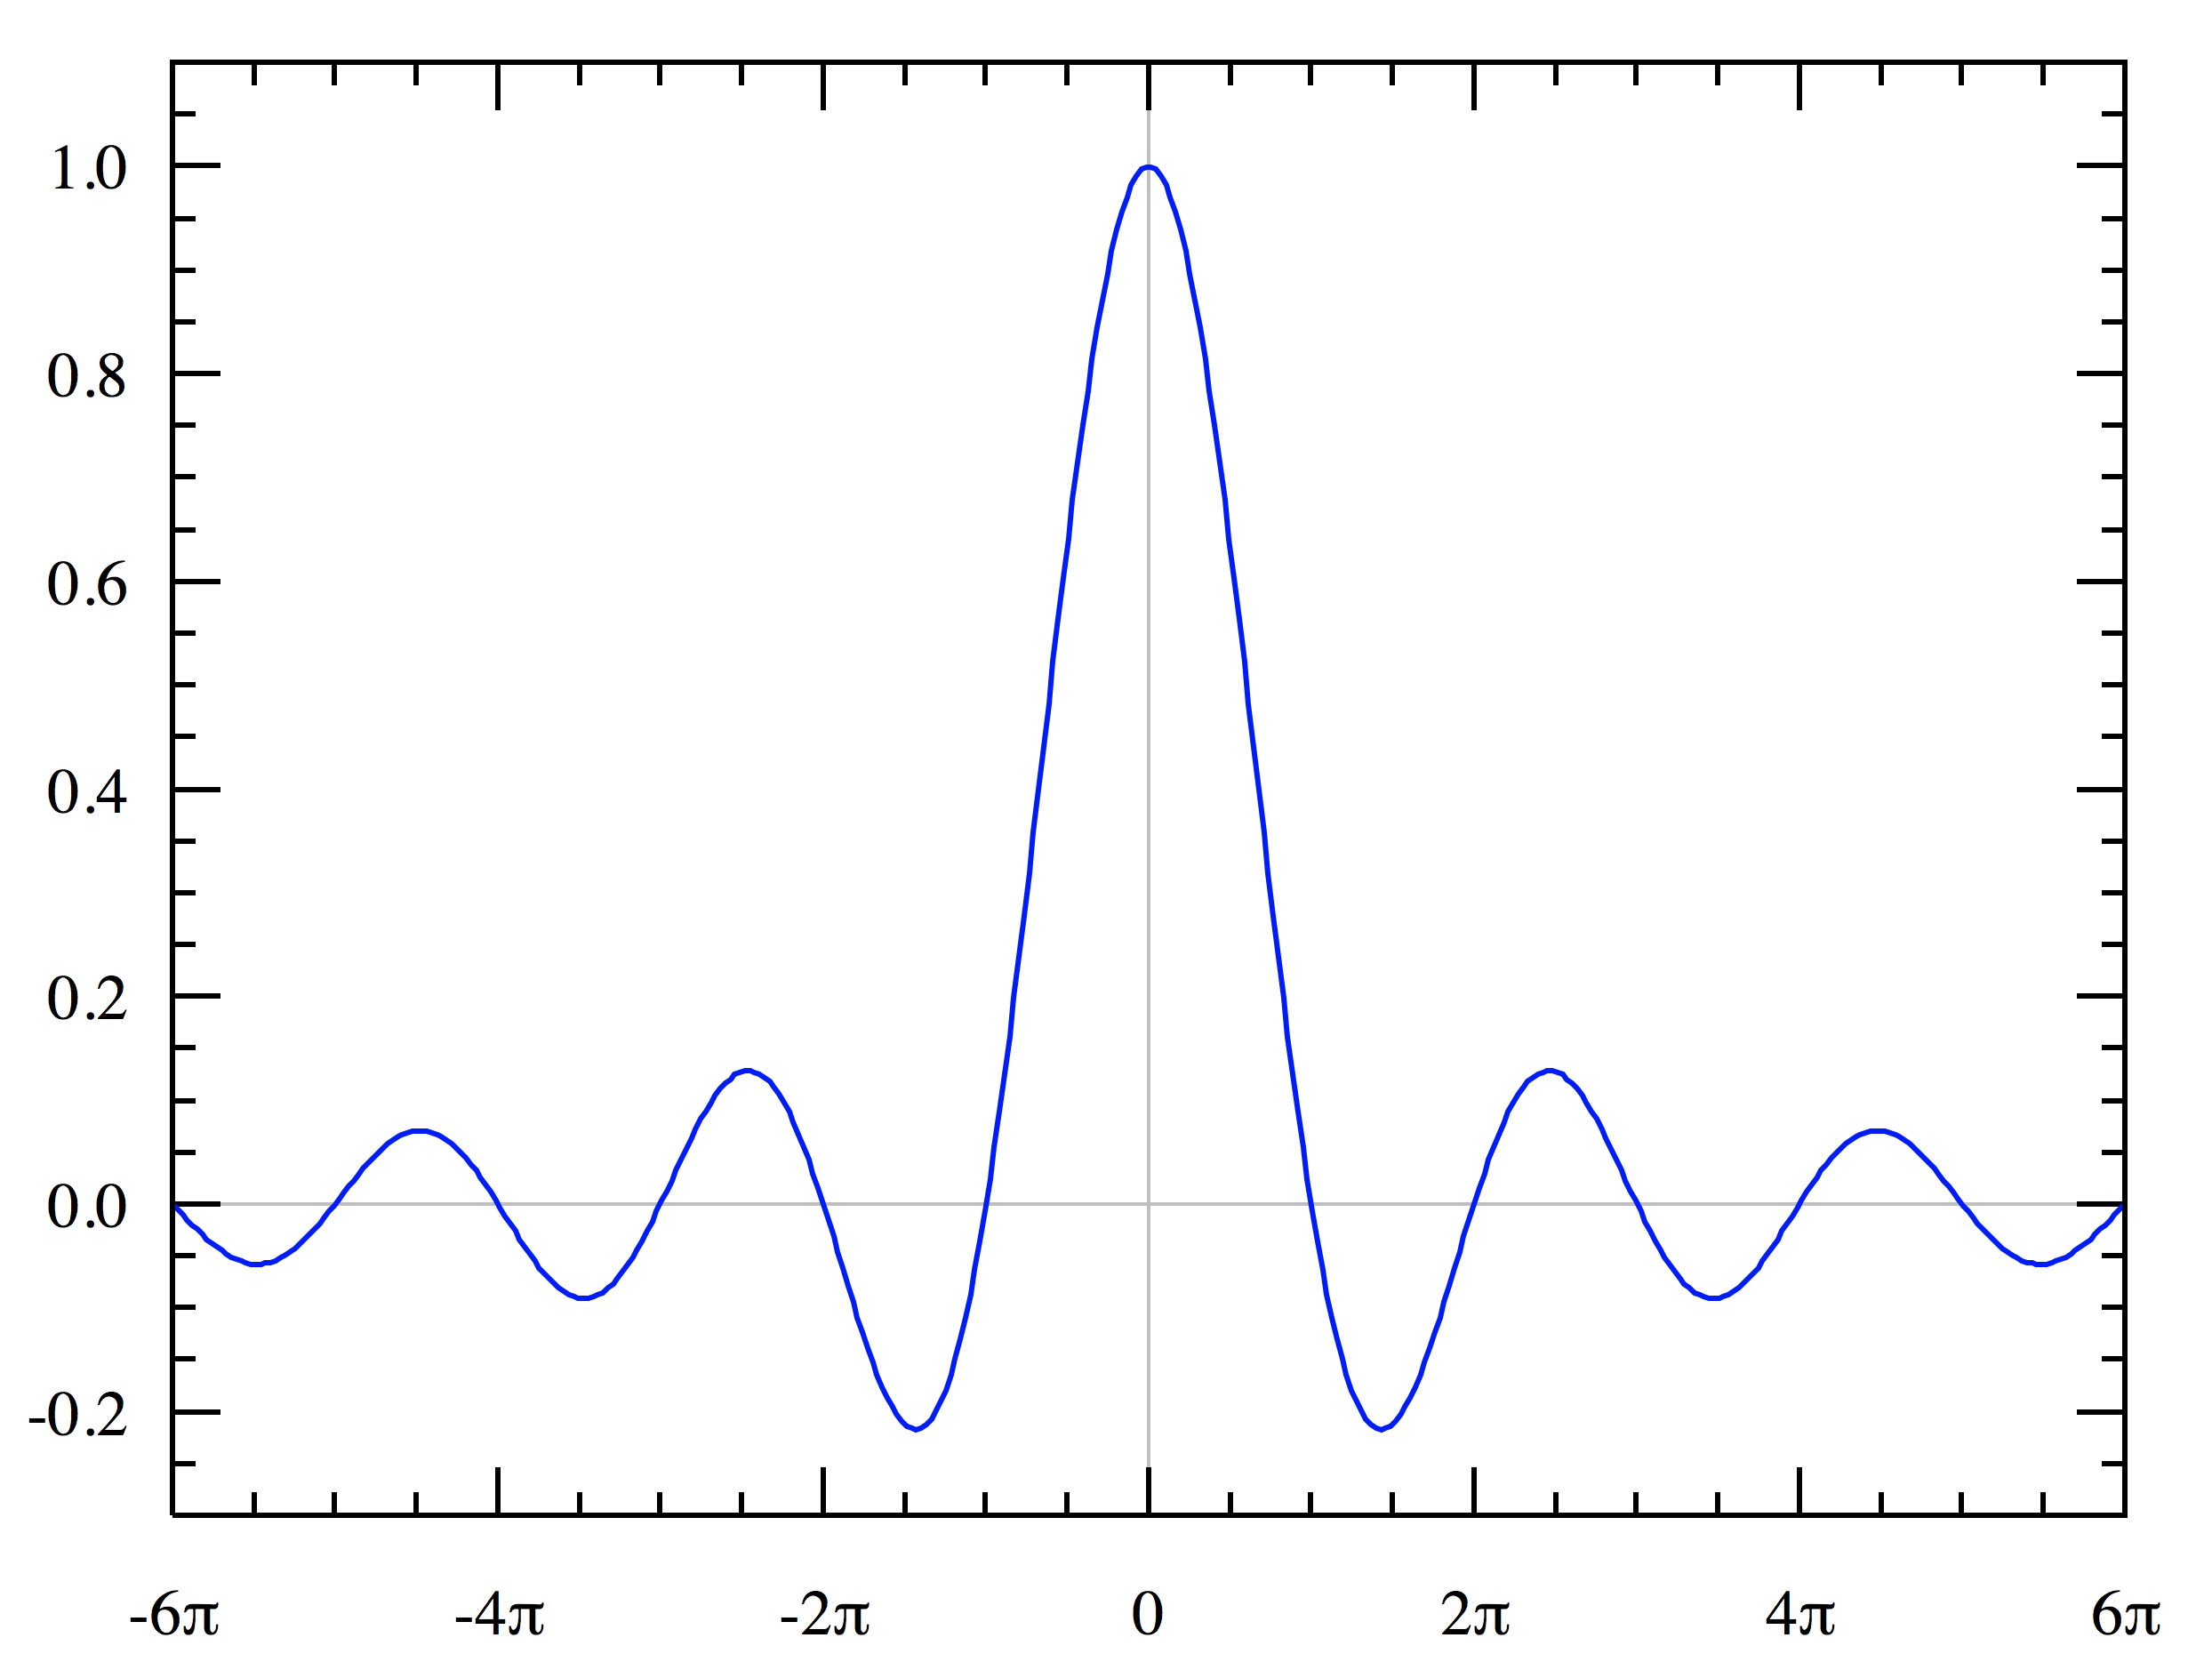
\includegraphics[width=3.5in]{image/sinc.png}
          \caption{sinc(x)}\label{pic_sinc}
        \end{figure} 

        不难看出, $osinc_+$ 与 $osinc_-$均具有函数形式:
        \begin{equation}
          sinc(x) = \frac{\sin(x)}{x}
        \end{equation}

        其具体函数图像如Fig.\ref{pic_sinc}所示.
         
        由上图可以看到, 当$x\to 0$时, 函数sinc(x)趋于最大值1.0. 而越远离原点, 函数值极值越小.
        因此, 若存在一值$\alpha$, 满足 |$\alpha|\gg 1$, 则$sinc(\alpha)$必满足
        $|sinc(\alpha)|\ll 1$

        

        \textbf{下面分两种情况讨论该问题.}
        \par
        
        \textbf{1.}  {\boldmath{$\omega_{mk}+\omega = \delta_\omega \to 0$}}\\
        
        此时, 
        \begin{subequations}
          \begin{align}
            osinc_+ & =  \frac{\sin(\delta_\omega t_0/2)}{\delta_\omega t_0/2}\\
            osinc_- & =  \frac{\sin(\omega t_0)}{\omega t_0}
          \end{align}
        \end{subequations}

        其中$osinc_+ \to 1$, 现分析$osinc_-$,

        \par
        令$x = \omega t_0$, $sinc(x)$的第一个零点位于 $x = \pi$处, 取光子为研究对象, 则有,
        \begin{equation}
          \begin{aligned}
            x & \iff \pi\\
            \omega t_0 & \iff \pi\\
            \frac{2\pi c}{\lambda}t_0 & \iff \pi\\
            t_0  & \iff \frac{\lambda}{2c}
          \end{aligned}
          \qquad\downarrow
        \end{equation}

        取光子波长为600nm, 则此时在$osinc_-$中, $sinc(x)$第一零点对应$t_0$的量级为: 
        $10^{-15}$s.也即飞秒级别.

        换言之, 只要微扰时间远大于飞秒级别, 就可以将$osinc_-$视为一相对于$osinc_+$的小量.

        这一条件在一般情况下是可以得到充分满足的!\footnote{不信你就问问我们的 ``吉大超快激光狗", 
        也就是传奇的 ``正则学长"...}

        因此, 在计算$P_{k\to m}$(以后将简写为$P_{km}$)\footnote{这里之所以再次加上箭头, 
        是因为需要再一次地强调量子态跃迁的方向}的过程中, 可以直接忽略$osinc_-$所在的一项, 
        而只考虑$osinc_+$
        所在的一项.

        因此就有:
        \begin{equation}
          \begin{aligned}
            P_{km}(t_0) & = \frac{|\hat{W}_{mk}|^2t_0^2}{\hbar^2}\cdot
            \frac{\sin^2[(\omega_{mk}+\omega)t_0/2]}{(\omega_{mk}+\omega)^2t_0^2/4}\\
            & = \frac{2|\hat{W}_{mk}|^2t_0}{\hbar^2}\cdot
            \frac{\sin^2[(\omega_{mk}+\omega)t_0/2]}{(\omega_{mk}+\omega)^2t_0/2}
          \end{aligned}
        \end{equation}

        利用一个数学上十分Trival的公式,
        \begin{equation}
          \label{deltalim}
          \pi\delta(x) = \lim_{k\to\infty}\frac{\sin^2(kx)}{kx^2}
        \end{equation}

        并做如下代换,
        \begin{equation}
          \begin{aligned}
            k & \longleftrightarrow t_0/2\\
            x & \longleftrightarrow (\omega_{mk}+\omega)
          \end{aligned}
        \end{equation}

        则有,
        \begin{equation}
          \begin{aligned}
            P_{km}(t_0) & = \frac{2\pi|\hat{W}_{mk}|^2t_0}{\hbar^2}
            \cdot\delta(\omega_{mk}+\omega)\\
            & = \frac{2\pi|\hat{W}_{mk}|^2t_0}{\hbar^2}
            \cdot\delta(\frac{E_m-E_k}{\hbar}+\omega)
          \end{aligned}
        \end{equation}

        再考虑到$\delta$函数的性质:
        \begin{equation}
          \delta(x) = |a|\delta(ax)
        \end{equation}

        最终,
        \begin{equation}
          \label{Pkm}
          P_{km}(t_0) = \frac{2\pi|\hat{W}_{mk}|^2t_0}{\hbar}
          \cdot\delta(E_m-E_k+\hbar\omega)
        \end{equation}
        
        注意观察\eqref{Pkm}, 可能产生如下疑虑: 在$E_m-E_k=-\hbar\omega$时, $\varphi_k\to 
        \varphi_m$态的跃迁概率
        为:
        \begin{equation}
          \label{sig_fin_P}
          P_{km}(t_0) = \frac{2\pi|\hat{W}_{mk}|^2t_0}{\hbar}\cdot\delta(0)
        \end{equation}

        方程中存在一个一阶无穷大$\delta(0)$, 而概率是无穷大是没有意义的!
        \par
        但是不要忘记一点, $\hat{W}_{mk}$是一个一阶无穷小量, 因此整体上, $P_{km}$是一个一阶无穷小!
        \par
        上述结论只对单色光成立, 一般情况下, 实验所得的光谱不可能是完全单色的, 而是应该在某一特定频率$\omega$
        附近有一个极其尖锐的分布. 该分布的尖锐程度和光的单色性有关. 
        \par
        下面我们讨论连续光谱对上述跃迁的几率的影响.
        \par
        回顾单色光谱的跃迁, 可以作如下理解: 假设有N个光子, $N\to\infty$, 对原子产生一个电磁微扰, 那么就会有
        N个原子受到微扰, 受微扰后跃迁的原子数为:
        \begin{equation}
          N_{km}(t_0) = N\cdot\frac{2\pi|\hat{W}_{mk}|^2t_0}{\hbar}
                         \cdot\delta(E_m-E_k+\hbar\omega)
        \end{equation}
        
        因此其跃迁概率为:
        \begin{equation}
          \label{content_P}
          \begin{aligned}
            P_{km}(t_0) &= \frac{1}{N}\left(N\cdot\frac{2\pi|\hat{W}_{mk}|^2t_0}{\hbar}
                           \cdot\delta(E_m-E_k+\hbar\omega)\right)\\
                        &= \frac{2\pi|\hat{W}_{mk}|^2t_0}{\hbar}
                           \cdot\delta(E_m-E_k+\hbar\omega)
          \end{aligned}
        \end{equation}
      
        这恰好就是前文中所得的结论.\footnote{这貌似是一句废话, 但是, 这一推导思想将在之后的连续谱中应用}
        
        在光子是连续谱情况下, 我们引入能量密度的概念, 也即, 对某一特殊频率附近, 其能量大小为:
        \begin{equation}
          \mathrm{d}U(\omega) = u(\omega)\mathrm{d}\omega
        \end{equation}
        
        $\mathrm{d}U$是处在某一$\omega$附近的总能量, 因此是$\mathrm{d}U$与$\omega$有关. 

        因此, 在某一特殊频率附近的光子数为:
        \begin{equation}
          \mathrm{d}n(\omega) = \frac{u(\omega)}{\hbar\omega}\mathrm{d}\omega
        \end{equation}

        将上式所得的光子数密度应用\eqref{content_P}式的思想, 可得:
        \par
        此时的跃迁概率为:
        \begin{equation}
          \begin{aligned}
            P_{km}(t_0) &= \dfrac{\int_{\omega-\Delta\omega}^{\omega+\Delta\omega}
                           \dfrac{2\pi|\hat{W}_{mk}|^2t_0}{\hbar}
                           \cdot\delta(E_m-E_k+\hbar\omega')
                           \dfrac{u(\omega')}{\hbar\omega'}\mathrm{d}\omega'}
                           {\int_{\omega-\Delta\omega}^{\omega+\Delta\omega}
                           \dfrac{u(\omega')}{\hbar\omega'}\mathrm{d}\omega'}\\
                        &= \dfrac{\dfrac{2\pi|\hat{W}_{mk}|^2t_0}{\hbar^2}u(\omega)}
                           {\int_{\omega-\Delta\omega}^{\omega+\Delta\omega}
                            \dfrac{\omega}{\omega'}u(\omega')\mathrm{d}\omega'}
          \end{aligned}
        \end{equation}

        若此时认为$\Delta\omega\to0$, 则
        \begin{equation}
          {\int_{\omega-\Delta\omega}^{\omega+\Delta\omega}
          \dfrac{\omega}{\omega'}u(\omega')\mathrm{d}\omega'} 
          =
          \dfrac{\omega}{\omega}u(\omega)\cdot2\Delta\omega
          =
          U(\omega)
        \end{equation}

        其中, $\omega = \dfrac{E_k-E_m}{\hbar}$, $U(\omega)$是体系关于体积的能量密度, 这里$\omega$的值其实是局限在一个很小的区域内的.
        \footnote{注意这里的$U$是$\omega$的函数是因为积分上下限的关系, 而不是说$U(\omega)$有某种
        关于$\omega$的能量密度的属性!}

        因此, 最终, 光子频率为连续谱的跃迁概率为:    
        \begin{equation}
          \label{con_fin_P}
          P_{km}(t_0) = \dfrac{2\pi|\hat{W}_{mk}|^2t_0}{\hbar^2}\cdot\frac{u(\omega)}{U(\omega)}
        \end{equation}
        
        对比\eqref{con_fin_P}与\eqref{sig_fin_P}, 不难发现, 二者的差别仅仅是将$\delta(0)$换作了
        $\dfrac{u(\omega)}{\hbar{}U(\omega)}$.\footnote{这也是十分好理解的! 因为在单值情况下, 
        $$u(\omega') = U(\omega)\cdot\delta(\omega'-\omega)$$  其中,$\hbar$已经被吸收进了$\delta$函数.}

        \begin{enumerate}[]
          \item 另外, \eqref{Pkm}实际上是十分有启发性的!
          \begin{enumerate}[--]
                      
            \item\emph{只有$\hbar\omega = E_k-E_m$时,才可以发生跃迁.也就是, $E_k$的能级必须高于
                  $E_m$, 也即, 此情况是量子体系的自发向下跃迁释放光子的过程.}
            \item \emph{微扰作用时间越长, 跃迁几率越大.}
            \item \emph{不同态的跃迁概率完全由含时微扰项$W_{mk}$决定.}
          \end{enumerate}
        \end{enumerate}

        \textbf{2.}  {\boldmath{$\omega_{mk}-\omega = \delta_\omega \to 0$}}
        \label{sec_transition_from}
 
        对于此种情况, 其分析过程与上述第一种情况完全类似. 

        或者说, 只需将第一种情况下的$\omega$替换为$-\omega$, 就可以及其简洁地转化为第二种情况.

        因此, 两者满足完全类似的跃迁几率.
        \begin{equation}
          \label{sec_tansition_equation}
          P_{km}(t_0) = \frac{2\pi|\hat{W}_{mk}|^2t_0}{\hbar}
          \cdot\delta(E_m-E_k-\hbar\omega) 
        \end{equation}
        \begin{enumerate}[]
          \item 类似的,上述公式也有如下几点启发.
          \begin{enumerate}[--]
            \item \emph{只有$\hbar\omega = E_m-E_k$时,才可以发生跃迁.也就是, $E_m$的能级必须高于
                  $E_k$, 也即, 此情况是量子体系吸收光子受激向上跃迁过程.}
            \item \emph{微扰作用时间越长, 跃迁几率越大.}
            \item \emph{不同态的跃迁概率完全由含时微扰项$W_{mk}$决定.}
          \end{enumerate}
        \end{enumerate}

        关于此种情况的光子连续谱与离散谱的跃迁概率表达式, 与上一种情况是完全类似的, 因此不再赘述.
         
        最后声明一点, 上述所有关于$P_{km}$的讨论都是在\eqref{deltalim}成立的前提下进行的.
        也即, $t_0$要较大. 于是我们说, $t_0$一般是足够大的, 因此我们可以没有有任何顾虑地使用\eqref{deltalim}式.
        但上述的表述只能给人一些安慰, 并不能产生实质性的信服力, 
        也不能提供任何关于$t_0$量级的信息.\\
        因此,下面对这个问题做具体分析.
        \begin{figure}[H]
          \centering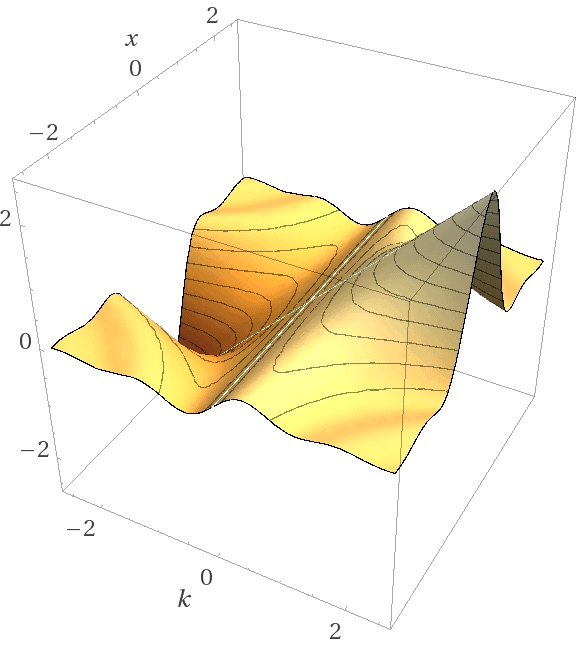
\includegraphics[width=2in]{image/delta.jpg}
          \caption{$\dfrac{\sin^2(kx)}{kx^2}$}\label{pic_delta}
        \end{figure} 

        Fig.\ref{pic_delta}为方程: 
        \begin{equation}
          z = \dfrac{\sin^2(kx)}{kx^2}
        \end{equation}
        
        的图像,
        \par
        将上述方程视为$x$的函数$z(x)$, 将$k$视为参数, 并对上述方程改变形式,
        \par
        得, 
        \begin{equation}
          \begin{aligned}
            z(x) & = \dfrac{\sin^2(kx)}{kx^2}\\ 
              & = k\cdot\left[\dfrac{\sin(kx)}{kx}\right]^2
          \end{aligned}
        \end{equation}

        利用半宽度标定其峰的尖锐程度.
        不难得到,
        \begin{equation}
          z_{max}(x) = z(0) = k
        \end{equation}

        其半宽度显然由方程:
        \begin{equation}
          \sin^2(kx) = \dfrac{1}{2}k^2x^2
        \end{equation}
        
        决定.

        令$kx = \alpha$
        则进一步地, 有,
        \begin{equation}
          \sin^2(\alpha) = \dfrac{1}{2}\alpha^2
        \end{equation}

        其解为:
        \begin{equation}
          \begin{aligned}
            \alpha_1 & = -1.392 \\
            \alpha_2 & = 0\text{(舍)}\\
            \alpha_3 & = 1.392
          \end{aligned}
        \end{equation}
      
        因此, 半宽度:
        \begin{equation}
          \Delta x = \dfrac{|\alpha_{root}|}{k} = \dfrac{1.392}{k}
        \end{equation}

        带入实际物理公式得,
        \begin{equation}
          \begin{aligned}
            \Delta E & = \dfrac{2.784}{t_0}\hbar\\
                     & = \dfrac{1.8325 \times 10^{-15} eV\cdot s}{t_0}
          \end{aligned}
        \end{equation}
        
        一般的, 取能级间隔($|E_k-E_m|$)是$0.1 \sim 10ev$量级.

        由上面的公式, 可分析得到, 只要$t_0$远大于飞秒级别, 就可以放心地使用
        \eqref{deltalim}做近似.
        
        
        \subsubsection{含时微扰的具体例子: 原子体系对光的辐射和吸收}
          原子体系对光的辐射和吸收主要有一下三种途径:

          \begin{enumerate}[*]
            \item 受激吸收: 选取原子中的两个能级$E_m, E_n$. 初态时, 原子多集中在能量较低的能级
                  $E_m$上. 此时给体系提供能量为$\hbar\omega$的光子, 且恰满足
                  $\hbar\omega=E_n-E_m$. 由此产生的原子吸收相应能量光子, 发生$E_m\to E_n$
                  的跃迁称为受激吸收.

            \item 受激辐射: 同样选取原子中的两个能级$E_m, E_n$. 初态时, 原子多集中在能量较高的能级
            $E_n$上. 此时给体系提供能量为$\hbar\omega$的光子, 且恰满足
            $\hbar\omega=E_n-E_m$. 原子吸收相应能量的单个光子后, 能级由$E_n$向下跃迁到$E_m$, 
            同时释放两个频率同为$\omega$的光子的过程称为受激辐射.
      
            \item 自发辐射: 选取原子中的两个能级$E_m, E_n$. 初态时, 原子多集中在能量较高的能级
            $E_n$上. 若经历一定的时间, 处于高能级$E_n$的粒子将会逐渐跃迁到低能级$E_n$, 并释放能量为
            $E_n-E_m$的光子. 这一过程被称为自发辐射.
          \end{enumerate}

          爱因斯坦研究了一定体系下, 上述三种辐射和吸收的关系.
          
          首先, 应该建立三种跃迁的定量关系. 考虑单位时间内跃迁的粒子数$N$影响因素, 可以得到如下结果:
          \begin{enumerate}[*]
            \item \emph{总粒子数}
            \item \emph{体系提供的在特定$\omega$频率下的光子 的 粒子数密度}
          \end{enumerate}
          
          上述的两个因素是十分好理解的. 打一个十分形象的比喻, 对于一个完全不懂台球而在打台球的人, 
          打进洞的台球的个数与两个因素有关: 台球的总数和击球的次数!

          而进一步的, 在此体系中, 对给定的两个能级, $\omega$的值实际上是固定的! 这就提醒我们, 
          可以将``光子在特定频率
          下的粒子数密度"这一因素换为: ``光子在特定频率下的能量密度''\footnote{不难看出, 
          光子的粒子数密度$n$与
          光子的能量密度$u$, 在一确定的角频率$\omega$下, 有如下简单的关系: $u(\omega) = 
          \hbar\omega\cdot n(\omega)$}

          因此, 就有如下三个公式\footnote{下标的写法参考\eqref{Pkm}中$\hat{W}_{mk}$的写法, 也即
          初态在后, 末态在前.}:
          \begin{subequations}
            \label{NABC}
            \begin{align}
              \dfrac{\mathrm{d}N_{nm}}{\mathrm{d}t} &= B_{nm}u(\omega)N_m \\
              \dfrac{\mathrm{d}N_{mn}}{\mathrm{d}t} &= B_{mn}u(\omega)N_n \\
              \dfrac{\mathrm{d}N_{mn}}{\mathrm{d}t} &= A_{mn}N_n
            \end{align}
          \end{subequations}

          注意, $E_n>E_m$.
          
          \textbf{
          先考虑如下体系, 一个光子源发出了一团达到热平衡的光子气体, 在此气体内部的某处固定地放置足够多的原子, 
          同时, 原子个数远小于光子个数以至于原子发生能级跃迁吸收或放出的光子不影响整个光子气体的平衡状态.}
          
          此时, 对于特定$\omega$下的光子的能量密度可由黑体辐射能量密度求得:  
          \begin{equation}
            \label{blackbody_radiation}
            u(\omega) = \frac{\hbar\omega^3}{\pi^2c^3}\cdot\frac{1}{\mathrm{e}^
            {\frac{\hbar\omega}{k_0T}}-1}
          \end{equation}
          
          可以想象, 在此光子热库下的原子体系, 其能级跃迁最终将到达动态平衡, 从而使整个原子体系处于
          热平衡状态. 热平衡的条件也可以总结为: 单位时间内向上跃迁的粒子数与向下跃迁的粒子数相等.
          
          也即, 
          \begin{equation}
            \label{Einstein_atom_transition_Equation}
            B_{nm}u(\omega)N_m =\left(B_{mn}u(\omega) + A_{mn}\right)N_n
          \end{equation}
       
          由\eqref{Einstein_atom_transition_Equation}可得, 
          \begin{equation}
            \label{simplification_of_EATE}
            u(\omega) = \dfrac{A_{mn}}{B_{nm}\dfrac{N_m}{N_n}-B_{mn}}
          \end{equation}
          
          注意到由于原子数足够多, 因此, 不同能级上原子的分布满足Boltzmann分布.

          即, 
          \begin{equation}
            \label{boltzmann_distribution}
            \dfrac{N_m}{N_n} = \mathrm{e}^{\frac{\hbar\omega}{k_0T}}
          \end{equation}

          其中, $\hbar\omega$是给定两原子之间的能级差. 其正好对应原子在两能级跃迁时吸收或辐射
          光子的能量, 因此用$\hbar\omega$代替$E_n-E_m$.

          联立\eqref{boltzmann_distribution}, \eqref{simplification_of_EATE}, 
          \eqref{blackbody_radiation}得到,
          \begin{subequations}
            \label{AB_res}
            \begin{align}
              B_{nm} &= B_{mn} \\
              A_{nm} &= \dfrac{\hbar\omega^3}{\pi^2c^3}B_{mn} 
            \end{align}
          \end{subequations}
          
          接着使用半经典理论, 分析光子作用在原子体系上发生受激吸收的过程.

          在经典理论中, 光子可以视为电磁波, 电磁波可以分解为电场与磁场. 从而, 光子对原子的作用可以视为电场与磁场对
          原子的作用.  
          
          \textbf{首先分析电场,} 
          
          一个光子所对应的电场部分作用于一个原子上, 此过程可视为一微扰. 则有:
          \begin{equation}
            \begin{aligned}
              \label{E_add_Energy}
              W_E(\vec{r},t) &= -q\vec{E}\cdot\vec{R}\\ 
                            &= -q\vec{R}\cdot\vec{E}\\ 
                            &= e\vec{R}\cdot\vec{E_0}\cos(\omega t'-\vec{k}\cdot\vec{r'}) 
            \end{aligned}
          \end{equation}
          
          其中, $\vec{R}$为原子中电子指向质子的距离矢量.
          
          这一结论可以做如下理解: 
          
          由于电场的存在, 原子体系产生了附加能, 而质子与电子之间的互相作用产生的能量显然是不
          包含在这一附加能里的. 为了求得此附加能, 可以设计这样一个体系, 该体系由一对带电量分别为$\pm{}e$的粒子组成, 
          规定由负带电粒子指向正带电粒子的矢量为$\vec{R}$.
          两带电体之间可视为没有相互作用, 或者相互作用可以忽略. 那么初始时刻, 体系总能量为0. 现对此体系加以电场,
          体系产生一个能量, 此时, 若将负带电粒子沿着$\vec{R}$移动到正带电粒子上, 那么, 体系电场附加能为0
          \footnote{因为此时相当于电场中没有了原子, 其等价的说法就是原子周围没有了电场!}.

          很明显, 在这一移动过程中, 体系的能量减小了$e\vec{E}\cdot\vec{R}$, 那么原来体系的总附加能即为
          \eqref{E_add_Energy}所示结果. 很显然, 此时, $\vec{R}$即为由电子指向质子的距离矢量! 
          
          为了使结果更加简单, 对电场结构进行进一步分析. 

          电磁波中, 电场的变化形式, 可写作:       
          \begin{equation}
            \vec{E} = \vec{E_0}\cos(\omega t'-\vec{k}\cdot\vec{r'}) 
          \end{equation}

          其中, $\vec{r'}$为光源到原子上电子的距离\footnote{光子影响原子能级实际上式通过与其电子作用引起的.},
          将其分解为指由光源指向原子核的矢量$\vec{r}$加上由原子核指向电子的矢量$\Delta\vec{r}$. 

          也即, 
          \begin{equation}
            \vec{r'} = \vec{r} + \vec{\Delta{}r}
          \end{equation}

          其中, $|\Delta\vec{r}|\ll |\vec{r}|$

          因此, 
          \begin{equation}
            \vec{E} = \vec{E_0}\cos(\omega t'-\vec{k}\cdot\vec{r}) 
          \end{equation}

          由于, 原子位置是一个定值, 因此, 上述公式$\cos$中的最后一项实际上是一个常数项因子, 不妨将其吸收到时间的相位中.
          则, \eqref{E_add_Energy}可进一步化简为:      
          \begin{equation}
            \label{E_add_Energy_simple}
            \begin{aligned}
              \hat{W}_E(\vec{r},t) &= e\vec{R}\cdot\vec{E_0}\cos(\omega t)\\
                            &= \dfrac{e\vec{E_0}\cdot\vec{R}}{2}
                            (\mathrm{e}^{i\omega{}t}+\mathrm{e}^{-i\omega{}t})
            \end{aligned}
          \end{equation}
          
          此即为光子电场部分对原子的微扰, 很显然着正式在前一小节中所讨论过的简谐微扰!
          
          
          这里可能会产生一个疑问: 不同位置的原子的跃迁几率是否会不同? 
          的确, 对于不同的原子, 其处于不同的位置上, 那么
          $t-t'$的差值也将不同, 这一差值将会直接影响\eqref{Cm1_simplize}中的积分上下限. 
          这就会导致, 不同原子的跃迁概率幅$C_m^{(1)}$不同. 但经过实际计算, 不难发现, 虽然概率幅不同, 
          但其只相差一个相位, 最终求得的跃迁概率仍是相同的! 所以上述过程中不同位置的原子受同样的光子的激发,
          其跃迁概率仍是相同的!
          
          \textbf{下面分析, 磁场的微扰:}

          首先分析磁场产生的附加能和电场产生附加能的大小关系, 取处在s态的电子为研究对象, 则其对于磁场的附加能只有其自旋磁矩提供
          \footnote{其轨道角动量为0, 轨道磁矩也就为0}.

          则其磁场附加能的形式为:
          \begin{equation}
            \hat{W}_B(\vec{r}, t) = \frac{e}{m_ec}\vec{B}\cdot\vec{s}
          \end{equation}
     
          由简单的电动力学知识\footnote{格里菲斯电动力学导论中文翻译版, 第三版, P242},平面电磁波电场与磁场的 
          关系为:
          \begin{equation}
            B(\vec{r}, t) = \frac{1}{c}\vec{k} \times \vec{E}
          \end{equation}

          将其应用到下面的推导中, 
          
          并注意到$\vec{r}$的量级可取波尔半径的量级$\vec{r}\sim{}a_0 = \dfrac{\hbar^2}{me^2}$
          \footnote{本小节中所有的推导使用的均为高斯单位制!}:
          \begin{equation}
            \begin{aligned}
              \frac{\hat{W}_E}{\hat{W}_B} &= \frac{|\dfrac{e}{m_ec}\vec{B}\cdot\vec{s}|}
                                                  {|e\vec{r}\cdot\vec{E}|}\\
                                          &= \frac{|\dfrac{e}{m_ec}\dfrac{1}{c}\vec{k}\times\vec{E}\cdot\vec{s}|}
                                                  {|e\vec{r}\cdot\vec{E}|}\\
                                          &\sim \frac{e^2|\vec{k}|}{c^2\hbar}\\
                                          &\sim \frac{e^2}{c\hbar}\cdot \frac{1}{c\lambda}\\
                                          &\sim \frac{\alpha}{c\lambda}
            \end{aligned}
          \end{equation}

          其中, $\alpha$被称为``精细结构常数'', 其值为$\dfrac{1}{137}$.
          
          因此, 电场产生的微扰大约是磁场产生微扰的$10^2\sim 10^3$倍.

          这一结论给之后的分析带来了极大的便利, 由于磁场产生的影响相对于电场如此之小, 以至于在之后的分析中, 
          我们可以直接忽略磁场对整个原子体系的影响!

          总结以上分析, 一个光子对原子能级的作用可以近似等效为一个简谐微扰! 其具体的微扰哈密顿量, 由\eqref{E_add_Energy_simple}决定.

          也即,
          \begin{equation}
            \hat{W}(\vec{r},t) = \dfrac{e\vec{E_0}\cdot\vec{R}}{2}
            (\mathrm{e}^{i\omega{}t}+\mathrm{e}^{-i\omega{}t}) 
          \end{equation}
          
          本节中讨论的跃迁是受激吸收, 也即对应\ref{sec_transition_from}小节中的第二种情况, 因此将上述微扰带入
          \eqref{sec_tansition_equation}中得到:     
          \begin{equation}
            P_{m\to{}n} = \frac{2\pi{}t_0}{\hbar}|\langle{}n|\frac{e\vec{E}_0\cdot\vec{R}}{2}|m\rangle|^2
            \cdot\delta(E_n-E_m-\hbar\omega)
          \end{equation}

          为了今后讨论的方便, 我们定义一个跃迁速率的概念, 其具体定义为: 单位时间内跃迁几率的大小.

          注意到, 这里讨论的是原子体系的受激吸收过程, 这表明, $E_n-E_m = \hbar\omega$这一条件已满足,   
        
          因此, 对于上述公式, 其平均的跃迁速率, 在$[0, t_0]$时间内, 为:
          \begin{equation}
            \begin{aligned}
              \mathcal{V}_{m\to{}n} &= \frac{2\pi}{\hbar}|\langle{}n|\frac{e\vec{E}_0\cdot\vec{R}}{2}|m\rangle|
                                        ^2\cdot\delta(0)\\
                                    &= \frac{\pi{}e^2E_0^2}{2\hbar}|\langle{}n|\frac{\vec{E}_0\cdot\vec{R}}{E_0}%
                                       |m\rangle|^2\cdot\delta(0)
            \end{aligned}
          \end{equation}

          引入电磁场能量密度, 并采用高斯单位制:  
          \begin{equation}
            \begin{aligned}
              U(\omega) &= \frac{1}{8\pi}\overline{E^2+B^2}\\ 
                        &= \frac{1}{4\pi}\overline{E^2} \\
                        &= \frac{1}{4\pi{}T}\int_0^TE_0^2\cos^2(\omega{}t)\mathrm{d}t\\
                        &= \frac{1}{8\pi}E_0^2
            \end{aligned}
          \end{equation}

          因此, 由上述推导有, 
          \begin{equation}
            E_0^2 = 8\pi{}U(\omega)
          \end{equation}

          将其带入跃迁速率表达式得:
          \begin{equation}
            \mathcal{V}_{m\to{}n} = \frac{4\pi^2e^2U(\omega)}{\hbar}
                                    |\langle{}n|\frac{\vec{E_0}\cdot\vec{R}}{E_0}|m\rangle|^2
                                    \cdot\delta(0)
          \end{equation}

          由于光子气体运动方向和电子相对原子核的位置都不确定, 因此, 其$\vec{E}$和$\vec{R}$的方向都不
          确定, 现在首先假设确定了$\vec{R}$, 讨论$\vec{E}$对这个确定位置的电偶极子的平均作用, 
          只需要对上述跃迁速率关于$\vec{E}$做积分. 

          同时注意到, 包含$\vec{E}$的项是, $\vec{E_0}/{E_0}$, 其长度是完全确定的, 即$r = 1$, 因此, 
          对$\vec{E}$的积分只是对一个$r = 1$的球壳进行的, 因此对任意$\vec{E}$的方向, 上述物理量的平均值为:
          \begin{equation}
            \begin{aligned}
              \overline{|\langle{}n|\frac{\vec{E_0}\cdot\vec{R}}{E_0}|m\rangle|^2}
              &= \overline{|\langle{}n|R\cos{(\theta')}|m\rangle|^2}\\
              &= |\langle{}n|R|m\rangle|^2 \cdot \frac{1}{4\pi}\int_0^\pi\cos^2\theta'\sin\theta'\mathrm{d}\theta'
                \int_0^{2\pi}\mathrm{d}\varphi\\
              &= \frac{1}{3}\cdot|\langle{}n|R|m\rangle|^2 
            \end{aligned}
          \end{equation}


          还应该注意到, 上述推导实际上规定了原子内电子与原子核的确定位置, 但实际上, $\vec{R}$并没有
          确定的方向, 要在最终的表达式中体现这一点, 只需要把标量$R$换为$\vec{R}$即可.
          
          您可能会像刚接触这个结论的我一样, 觉得这难以接受, 但是只需换一种思考方式, 这个问题就
          很好理解了. 首先考虑二维平面的情况, 要确定两个方向自由但是固定长度固定的自由向量, 只需要两个参
          数$\theta_{abs}, \theta_{rel}$, 其中$\theta_{abs}$是一个向量与坐标轴的夹角, $\theta_{rel}$
          是两个向量之间的夹角. 在前面的讨论中, 我们实际上是固定了$\theta_{abs}$而只讨论了$\theta_{rel}$. 
          因此, 要体现$\theta_{abs}$的作用, 只需要在最后的结果中将所得的标量变为矢量即可! 也就说, 我们认为
          所有的结果都会一样的, 即使$\theta_{abs}$不同\footnote{由此推广到三维的情况, 结论也是类似的, 
          只不过此时需要4个参量, 2个相对角度, 2个绝对角度}.

          因此综合上述分析, 得到, 在该体系下的关于光子原子运动方向的平均跃迁概率为:
          \begin{equation}
            \label{V_single}
            \mathcal{V}_{m\to{}n} = \frac{4\pi^2e^2U(\omega)}{3\hbar}
                                  |\langle{}n|\vec{R}|m\rangle|^2
                                    \cdot\delta(0)
          \end{equation}
          
          应用\eqref{con_fin_P}式的结果, 可以得到, 在光子为连续谱的情况下, 
          \begin{equation}
            \label{V_content}
            \begin{aligned}
                \mathcal{V}_{m\to{}n} &= \frac{4\pi^2e^2U(\omega)}{3\hbar^2}
                                        |\langle{}n|\vec{R}|m\rangle|^2
                                        \cdot\frac{u(\omega)}{U(\omega)}\\
                                      &= \frac{4\pi^2e^2u(\omega)}{3\hbar^2}
                                        |\langle{}n|\vec{R}|m\rangle|^2\\
                                      &= \frac{4\pi^2u(\omega)}{3\hbar^2}
                                      |\langle{}n|\vec{D}|m\rangle|^2
            \end{aligned}      
          \end{equation}

          其中$\vec{D}$为电偶极矩张量.

          同时, 此跃迁速率也可由爱因斯坦的半定量公式写出, 由受激吸收表达式,         
          \begin{equation}
            \label{exp_V_content}
            \dfrac{\mathrm{d}N_{nm}}{N_m\mathrm{d}t} = -\dfrac{\mathrm{d}N_{m}}{N_m\mathrm{d}t}
            = B_{nm}u(\omega) = \mathcal{V}_{m\to{}n}
          \end{equation}
          
          对上式进一步求解得:
          \begin{equation}
            N_m(t) = N_m(0)\cdot\mathrm{e}^{-B_{nm}u(\omega)t}
          \end{equation}
          
          可见, 在受激吸收过程中, 低能级上的粒子数是随e指数递减的!
        
          另外, 通过对比\eqref{exp_V_content} 与 \eqref{V_content}可得:
          \begin{equation} 
            B_{nm} = \frac{4\pi^2}{3\hbar^2}|\langle{}n|\vec{D}|m\rangle|^2
          \end{equation}

          再由, \eqref{AB_res}可得:
          \begin{subequations}
            \label{fin_AB}
            \begin{align}
              B_{nm} &= \frac{4\pi^2}{3\hbar^2}|\langle{}n|\vec{D}|m\rangle|^2\\
              B_{nm} &= \frac{4\pi^2}{3\hbar^2}|\langle{}n|\vec{D}|m\rangle|^2\\
              A_{nm} &= \frac{4\omega^3}{3\hbar{}c^3}|\langle{}n|\vec{D}|m\rangle|^2
            \end{align}
          \end{subequations}
          
          上式说明, Einstain常数A, B的取值只与该体系的平均电偶极矩有关.

        \subsubsection{原子内部电子能级的跃迁选择定则}
          有了上面的分析作为基础, 我们就可以进一步探讨在原子物理中学过的所谓的``跃迁选择定则''了.

          由\eqref{AB_res}可知, 要产生跃迁, 必须要使$A_{nm}, B_{nm}, B_{mn}$不为零! 再参考
          \eqref{fin_AB}, 可以, 跃迁选择定则应该是来源于关系:
          \begin{equation}
            \label{transition_request}
            \langle{}n|\vec{R}|m\rangle \ne 0
          \end{equation}

          下面以氢原子为例, 讨论其跃迁选择定则:

          假设目前有两个氢原子的量子态:
          \begin{equation}
            \begin{aligned}
              &|n,l,m_l,m_s\rangle\\
              &|n',l',m_l',m_s'\rangle \notag
            \end{aligned}
          \end{equation}

          下面讨论, 算符$\vec{R}$对量子态的作用:
          \begin{subequations}
            \label{rxyz}
            \begin{align}
              \vec{R} &= x\hat{e}_x + y\hat{e}_y + z\hat{e}_z\\
                    x &= \frac{R(\mathrm{e}^{i\varphi}+\mathrm{e}^{-i\varphi})}{2}\sin(\theta)\\
                    y &= \frac{R(\mathrm{e}^{i\varphi}-\mathrm{e}^{-i\varphi})}{2i}\sin(\theta)\\
                    z &= R\cos(\theta)
            \end{align}
          \end{subequations}
          
          同时还有, 
          \begin{subequations}
            \label{sincos_H}
            \begin{align}
              &\sin(\theta)\mathrm{e}^{\pm{}i\varphi}|n,l,m_l,m_s\rangle \notag\\
              &= C_1|n,l+1,m_l\pm1,m_s\rangle + C_2|n,l-1,m_l\pm1,m_s\rangle\\
              &\cos(\theta)|n,l,m_l,m_s\rangle \notag \\
              &= D_1|n,l+1,m_l,m_s\rangle + D_2|n,l-1,m_l,m_s\rangle
            \end{align}
          \end{subequations}

          由\eqref{rxyz}和\eqref{sincos_H}可以得到, 如果将$\vec{R}$作用在量子态
          $|n,l,m_l,m_s\rangle$上, 得到的结果将是以下几个本征态线性叠加的形式.
          \begin{equation}
            \label{target_transition}
            \begin{aligned}
              &|n,l+1,m_l,m_s\rangle\\
              &|n,l-1,m_l,m_s\rangle\\
              &|n,l+1,m_l+1,m_s\rangle\\
              &|n,l-1,m_l+1,m_s\rangle\\
              &|n,l+1,m_l-1,m_s\rangle\\
              &|n,l-1,m_l-1,m_s\rangle
            \end{aligned}
          \end{equation}

          因此, 为了使条件\eqref{transition_request}得到满足, 如果初始的态是$|m\rangle$, 
          跃迁的目标态$|n\rangle$就必须是\eqref{target_transition}中的一个.
          
          将上面的描述总结为具体的规则, 就成为所谓的\textbf{跃迁选择定则:}

          \begin{enumerate}[*]
            \centering
            \item $\Delta{}m_s = 0$
            \item $\Delta{}l = \pm1$ 
            \item $\Delta{}m_l = 0, \pm1$
          \end{enumerate}
          
          这里, 您可能会产生一个问题, 上述规则为什么不包含$\Delta{}n = 0$这一约束?

          有这个疑问是因为, 由\eqref{sincos_H}可以看出, 算符$\vec{R}$对$m_s$和$n$的均不会产生影响, 
          因此, 这两个量子数都应该满足初末态差值为零的要求!

          这个问题的根源实际上是前面采用的写法太过迷惑性导致的. 如果将上述本征矢写成波函数的形式, 结果将更加清楚.
          \begin{equation}
            \langle{}r,\theta,\varphi,\chi|n,l,m_l,m_s\rangle = R_{nl}(r)Y_l^m(\theta,\varphi)\chi_s
          \end{equation}

          于是, 这里就可以看到, 前面我们所谓的$\mathrm{e}^{\pm{}i\varphi}\sin{\theta}$和$\cos{\theta}$对态矢的作用, 仅仅是对
          球谐函数$Y_l^m$的作用, 他们是不会改变径向函数$R_{nl}(r)$中的$l$指标的. 换句话说, 氢原子的本征态被$\vec{R}$作用过之后, 并不会得到一个氢原子新的
          本征态. 也正是因为这样, 如果要满足球谐函数不正交的条件, 也就是跃迁末态的$l'm'$要和跃迁初态被$\vec{R}$作用之后得到的球谐函数的$lm$保持一致, 那么跃迁
          末态径向函数$R_{n'l'}(r)$中的$l$与跃迁初态被$\vec{R}$作用之后得到的径向函数$R_{nl}$中的$l$就一定是不同的(或更确切的说是相差1)! 
          两个不同$l$的广义拉盖尔函数正交性是不容易被满足的. 因此, 跃迁选择定则中才没有对量子数$n$的限制. 也就是:  
          \begin{equation} 
            \int_0^{\infty}R_{n,l}^*(r)\cdot{}R_{n',l\pm1}(r)r^2\mathrm{d}r \ne 0
          \end{equation}

          然而, 这一点放在自旋量子数$m_s$上就完全不同了, $m_s$不同必然导致本征矢正交, 进而跃迁几率为$0$.\footnote{只有一个指标, 不像径向波函数中一样, 有$nl$两个指标.}
          因此对自旋磁量子数的约束是要有的.

        \subsubsection{常微扰与黄金规则}
          假设存在一常微扰, 其形式是:
          \begin{equation}
            \hat{W}(x, t) = 
            \begin{cases}
              0 & t<0\;or\;t>t_0,  \\
              \hat{W}(x) &  t \in [0, t_0]
            \end{cases}
          \end{equation}
          
          首先考虑简谐微扰的形式:      
          \begin{equation}
          \hat{W}(x, t) = \hat{W}(x)\mathrm{e}^{i\omega{}t} 
                        + \hat{W}^\dag(x)\mathrm{e}^{-i\omega{}t} \qquad t \in (0, t_0)
          \end{equation}
         
          其解已在\ref{jianxieweirao}小节中完全推出.  

          不难发现, 所谓的常微扰, 正是简谐微扰中的$\omega = 0$的情况.

          因此直接将$\omega = 0$这一条件带入\ref{jianxieweirao}小节所得的结果中, 
          就可以推导得到, 常微扰的跃迁速率为:
          \begin{equation}
            \label{gold_law}
            \mathcal{V}_{k\to{}m} = \frac{2\pi|\hat{W}_{mk}|^2}{\hbar}\cdot\delta(E_n-E_m)
          \end{equation}

          推广到连续的情况:
          \par
          您可能会想, 将我们之前得到的关于连续谱和离散谱的关系带入, 也即:
          \begin{equation}
            \mathcal{V}_{k\to{}m} = \frac{2\pi|\hat{W}_{mk}|^2}{\hbar^2}\cdot\frac{u(\omega)}{U(\omega)}
          \end{equation}
          
          就已经简洁地解决这个问题了!

          但这其实是错误的, 因为由\eqref{gold_law}可见, 只有当$E_n, E_m$几乎相等的时候, 才可以发生跃迁.
          也即, 此时可以认为能级是连续的. $\omega$是否连续无关紧要. 因此, 这里所谓的连续性情况是指能级连续, 
          与之前的光子频率连续是不同的.

          重新分析, 在此种连续情况下体系的跃迁速率.
          假设可供其跃迁的态有多个, 则:
          \begin{equation}
            \begin{aligned}
              \mathcal{V}_{all} &= \sum_m \mathcal{V}_{k\to{}m}\\
                                &= \sum_m \frac{2\pi}{\hbar}|\hat{W}_{mk}|^2\cdot\delta(E_m-E_k)
            \end{aligned} 
          \end{equation}

          由前文表述, 原子能谱可以视为是连续的, 将上述离散求和化为积分.
          \par
          只需要:
          \begin{equation}
            \sum_m \to \int_{E_k-\Delta{}E}^{E_k+\Delta{}E}\rho(E_m)\mathrm{d}E_m\notag
          \end{equation}

          其中, $\rho(E_m)$为原子在其能级$E_m$附近的态密度.

          因此, 最终, 连续原子能谱下体系的跃迁速率为:
          \begin{equation}
            \begin{aligned}
              \mathcal{V}_{all} &= \int_{E_k-\Delta{}E}^{E_k+\Delta{}E}\rho(E_m)
              \frac{2\pi}{\hbar}|\hat{W}_{mk}|^2\cdot\delta(E_m-E_k)\mathrm{d}E_m\\
                                &= \frac{2\pi}{\hbar}|\hat{W}_{mk}|^2\rho(E_k)
            \end{aligned}
          \end{equation}

          注意到, 积分上下限中的$\Delta{}E$可以在开区间$(0, +\infty)$中取任意值而不改变最终的积分值.
          这说明, 连续能级除了在区间$(E_i-\varepsilon, E_i+\varepsilon), \varepsilon\to0$中
          跃迁速率不是零外, 其余区域跃迁速率均为零!

          我们将区间$(E_i-\varepsilon, E_i+\varepsilon), \varepsilon\to0$抠去$E_i$点后的区间
          视为一个整体的态, 那么体系由初态$E_k$跃迁到该态的概率就是:         
          \begin{equation}
            \label{Fermis_Golden_rule}
            \mathcal{V}_{all} = \frac{2\pi}{\hbar}|\hat{W}_{mk}|^2\rho(E_k)
          \end{equation} 

          \eqref{Fermis_Golden_rule}式即为传奇的\textbf{``费米黄金规则''(Fermis Golden rule)}

        \subsubsection{激光的产生原理}
          激光实际上就是原子``受激辐射''产生的类似于光放大效果的不断累积.

          要产生激光就需要有粒子数翻转机制.
        \subsubsection{激发态寿命}
          最后研究``自发辐射''所引起的一些现象.
          
          由\eqref{NABC}中关于自发辐射的式子:
          \begin{equation}
            \begin{aligned}
              A_{mn}N_n &= \dfrac{\mathrm{d}N_{mn}}{\mathrm{d}t} \\ 
                        &= -\dfrac{\mathrm{d}N_{n}}{\mathrm{d}t}                           
            \end{aligned}
          \end{equation}

          解得:
          \begin{equation}
            N_n(t) = N_n(0)\mathrm{e}^{-A_{mn}t}
          \end{equation}
          
          定义原子寿命为$\tau$, 并满足:
          \begin{equation}
            N_n(\tau) = N_n(0)\mathrm{e}^{-1}
          \end{equation}
          
          也即:
          \begin{equation}
            \tau = \frac{1}{A_{mn}}
          \end{equation}

          如果有多个能级可供跃迁, 如: 由第4能级向1,2,3能级跃迁. 则第四能级的寿命就可以写作:
          \begin{equation}
            \tau = \frac{1}{A_{14}+A_{24}+A_{34}}
          \end{equation}

        \subsubsection{突变含时量子体系}
          前文中, 我们分析了许多关于含时微扰的内容. 这一节我们将认识另一种含时量子体系: 突变含时量子体系.

          其具体的形式如下:
          \begin{equation}
            \hat{H}(x, t) = 
            \begin{cases}
              \hat{H}_1(x) & t \in [0, t_0],\\
              \hat{H}_2(x) & t \in (t_0, \infty)
            \end{cases}
          \end{equation}

          下面举一个具体的突变含时量子体系的例子:
          \par
          \emph{假设在一宽为$a$的无限深方势阱有一粒子处在基态, 在$t=0$时刻, 方势阱的宽度突然增大到
          $2a$, 求在$t>0$的某一时刻观测该量子体系, 其有可能坍缩在哪些态上, 概率各是多少?}

          由上述描述可知, 体系的哈密顿量具体形式为:
          \begin{equation}
            \hat{H}(x, t) = 
            \begin{cases}
              \hat{H}_a(x) & t < 0,\\
              \hat{H}_{2a}(x) & t > 0
            \end{cases}
          \end{equation}

          开始时, 体系的能量本征态为:
          \begin{equation}
            \varphi^a_n(x) = 
            \begin{cases}
              \sqrt{\dfrac{2}{a}}\sin(\dfrac{n\pi{}x}{a}) & ,x\in[0, a],\\
              0 & ,elsewhere
            \end{cases}
          \end{equation}

          体系处在$\hat{H}_a, n=1$的基态上:
          \begin{equation}
            \psi(x, 0) = \sqrt{\frac{2}{a}}\sin(\frac{\pi{}x}{a})
          \end{equation}

          $\hat{H}$突变时, 体系的量子态不会变化.

          突变后, 体系的能量本征态变为:
          \begin{equation}
            \varphi^{2a}_n(x) = 
            \begin{cases}
              \sqrt{\dfrac{1}{a}}\sin(\dfrac{n\pi{}x}{2a}) & ,x\in[0, 2a],\\
              0 & ,elsewhere
            \end{cases}
          \end{equation}

          将体系的初态$\psi(x, 0)$向新的本征态上展开:
          \begin{equation}
            \varphi_1^{a} = \sum_{m=1}^\infty{}C_m\varphi_m^{2a}
          \end{equation}
          
          方程两侧同时乘$\varphi^{2a}_n$并在全空间积分后化简得到:
          \begin{equation}
            \begin{aligned}
              C_n &= \int_0^a \sqrt{\dfrac{1}{a}}\sin(\dfrac{n\pi{}x}{2a})
                             \sqrt{\frac{2}{a}}\sin(\frac{\pi{}x}{a})
                             \mathrm{d}x\\
                  &= \dfrac{2\sqrt{2}}{n+2}\cdot\dfrac{\sin\dfrac{(n-2)\pi}{2}}{\dfrac{(n-2)\pi}{2}}
            \end{aligned}                           
          \end{equation}

          简要的列出几个系数的数值:$C_1 = -0.6, C_2 = 1/\sqrt{2}, C_3 = 0.36$. 

          同时注意到, 系数$C_n$实际上是由$\dfrac{1}{x}$与$sinc(x)$两个函数乘积的结果, 且在$n=2$时$sinc(x)$
          取到极大值, 也就是说, 如果基态系数$C_1$的绝对值比$C_2$的绝对值小, 那么$C_2$的绝对值将是所有
          投影本征态中概率幅最大的! 进一步的, 该体系最终坍缩在$\varphi_2^{2a}$态上的几率也将最大.

          事实也确实如此!

          经过简单的计算就可得到, 体系坍缩在$\varphi_2^{2a}$态上的几率最大, 为$0.5$.

          更有意思的是, 在区间$[0,a]$内, $\varphi_2^{2a}$态与初态$\varphi_1^{a}$的函数图像恰好重合!
          \footnote{量子态不愿意改变太多?惯性?勒夏特效应?楞次定律?负反馈?或是巧合?}

    \subsection{绝热近似} 
      \subsubsection{绝热定理的引入}
        \textbf{
        绝热定理: 假设体系哈密顿量$\hat{H}^i$绝热变化到$\hat{H}^f$, 且在这个过程中, 哈密顿量能谱分立不简并. 若初始时, 体系处于
        $\hat{H}^i$的第$n$个本征态, 则绝热演化后, 其仍处于$\hat{H}^f$的第$n$个本征态上.}
        \par
        下面对上述定理进行证明:
        \par
        若体系的哈密顿量含时, 则在每一个瞬时, 对于一个确定的不含时的$\hat{H}(t_s)$
        \footnote{这里使用$t_s$是为了指明不同瞬时不同定态的变化和体系整体态的变化是不同的}, 
        体系存在定态.
        \par
        应注意的是, 这一定态的引入只是为了方便, 其并不是整个过程中的定态.
        \par
        事实上, 如果$\hat{H}$含时, 且是非绝热过程, 则整个体系并不存在所谓的定态.
        \par
        对某一瞬时列出定态薛定谔方程:
        \begin{equation}
          \hat{H}(t_s)\varphi_n(t_s) = E_n(t_s)\varphi_n(t_s)
        \end{equation}
        
        对整个体系而言, 其变化满足薛定谔方程:     
        \begin{equation}
          i\hbar\dfrac{\partial}{\partial{}t}\psi(x, t) = \hat{H}(t)\psi(x, t)
        \end{equation}
      
        取$t = t_s$, 将$\psi(x, t)$向$\varphi_n(t_s)$上展开.则有,
        \begin{equation}
          \label{origin_out}
          \begin{aligned}
            \psi(x, t_s) &= \sum_nC_n(t_s)\varphi_n(t_s)\mathrm{e}^{i\theta_n(t_s)t_s}\\
            \theta(t_s)_n &= -\frac{1}{\hbar}\int_0^{t_s}E_n(t')\mathrm{d}t'
          \end{aligned}
        \end{equation}

        要注意, 上式中的系数$C_n(t_s)$是相当重要的. 对于单个$\varphi_n(t_s)$, 其本身并不满足薛定谔方程. 
        但通过$C_n(t_s)$的变换和粘合, 最终形成的整体, 也就是$\psi(x, t)$, 是满足薛定谔方程的!
        \par
        想清楚这一点是很重要的, 尤其是在后面几何相因子的分析中.
        \par 
        这个地方其实会产生很多疑问, 下面简单的列几个:
        \par

        \begin{enumerate}[*]
          \item 问:前面说这个独立的态$\varphi_n$不满足薛定谔方程, 这也太绝对了吧, 比如, 如果初态是定态的话,
          那么这个定态的后续变化肯定是满足哈密顿量是$\hat{H}(t)$的薛定谔方程的, 不是吗?
          \item 答: 你理解的有问题, \textbf{仔细拼品一品哦, ``定态随时间的变化''
          \footnote{仔细品一品, 不考虑相因子, 定态怎么会随时间变化?这种变化到底是由什么决定的?}
          和``量子态随时间的演变'', 这其实完全是两个不同的概念啊, 不能混为一谈的!}
          \item 问: 怎么不一样了? 不都是关于时间的偏导数吗?
          \item 答: 别把自己绕进去啊, \textbf{我们前面也提到了, 体系整体的量子态关于时间演变的信
          息是储存在系数$C_n$中的. 本征矢只是一个基矢, 
          相当于向量空间中的基坐标$\hat{e}_x, \hat{e}_y, \hat{e}_z$, 他们的选取完全是
          任意的, 他们的变化也完全是可以人为的规定的!因此不可能满足薛定谔方程!}
          \item 问:什么? 你是说$\varphi_n(t_s)$随时间的变化是完全可以人为规定的? 怎么会!
          \item 答:没错啊, 因为这里为了方便计算, 我们约定取$\hat{H}(t_s)$的本征矢
          $\varphi_n(t_s)$作为展开的基矢是吧. 所以, 我们完全可以通过调控
          $\hat{H}(t_s)$来规定基矢的选择!这样不就完全人为规定了$\varphi_n(t_s)$随时间的变化了吗?
          这也正是我们这里使用$t_s$而不是$t$去标定$\varphi_n$随时间变换的原因啊!\\
          但是, 要注意哦, 我们有能力随心所欲地规定基矢的选取, 但是要操控系数$C_n(t_s), n=1,2,3...$的变化,
          还要看薛定谔方程给不给面子哦!
          \item 你是说...一个薛定谔方程可以同时规定$n$个系数的变化?
          \item 对啊, 不要被$n$给迷惑了, 这里实际上就是一个态, 先用薛定谔方程做一做变换, 
          再展开到某个规定好了的基矢上. 所以总体来说, 就是一个薛定谔方程规定了$n$个系数的变化. 
        \end{enumerate}
        \par
        由于作为一个整体, $\psi(x, t)$满足薛定谔方程, 所以\eqref{origin_out}中的$t_s$就不必再为强
        调单个$\varphi_n(t_s)$作为瞬时定态不满足薛定谔方程这一特殊性质而继续存在了, 可以将其直接换为$t$.
        \begin{equation} 
          \begin{aligned}
            \psi(x, t) &= \sum_nC_n(t)\varphi_n(t)\mathrm{e}^{i\theta_n(t)t}\\
            \theta(t)_n &= -\frac{1}{\hbar}\int_0^{t}E_n(t')\mathrm{d}t'
          \end{aligned}
        \end{equation}
        
        联立上述几式得, 
        \begin{equation}
          i\hbar\sum_n\left[C_n'(t)\varphi_n(t)+C_n(t)\varphi_n'(t)+C_n\varphi_ni\theta_n'(t)\right]
          \mathrm{e}^{i\theta_n(t)t} = \hat{H}\sum_nC_n(t)\varphi_n(t)\mathrm{e}^{i\theta(t)t}
        \end{equation}

        化简得:
        \begin{equation}
          i\hbar\sum_n\left[C_n'(t)\varphi_n(t)+C_n(t)\varphi_n'(t)+0\right]
          \mathrm{e}^{i\theta_n(t)t} =0
        \end{equation}

        方程两边同时作用一个左矢$\langle\varphi_m(t)|$,得:    
        \begin{equation}
          \label{complex_Cm}
          \begin{aligned}
            \dfrac{\partial{}C_m(t)}{\partial{}t}\mathrm{e}^{i\theta_m(t)t} &= -\sum_nC_n(t)
            \langle\varphi_m|\varphi_n'\rangle\mathrm{e}^{i\theta_n(t)t}\\
            \dfrac{\partial{}C_m(t)}{\partial{}t} &= -\sum_nC_n(t)\langle\varphi_m|\varphi_n'\rangle
            \mathrm{e}^{i(\theta_n(t)-\theta_m(t))t}\\
            &= -C_m(t)\langle\varphi_m(t)|\varphi_m'(t)\rangle - \sum_n^{n\ne{}m}C_n(t)
            \langle\varphi_m|\varphi_n'\rangle\mathrm{e}^{i(\theta_n(t)-\theta_m(t))t}
          \end{aligned}
        \end{equation}
      
        现研究, 在绝热过程中, $\langle\varphi_m|\varphi_n'\rangle$的大小问题.
        \par
        注意由前面的分析可知, 这里的$\varphi_n'$是不满足含时薛定谔方程的.
        \par
        因此使用定态薛定谔方程:
        \begin{equation}
          \hat{H}(t_s)\varphi_n(t_s) = E_n(t_s)\varphi_n(t_s)  
        \end{equation}

        方程两边同时对$t_s$\footnote{这里不牵扯薛定谔方程, 所以$t, t_s$已经可以混用了}求偏导数得到:
        \begin{equation}
          H'\varphi_n + H\varphi_n' = E_n'\varphi_n + E_n\varphi_n'
        \end{equation}

        方程两边同时作用一个左矢$\langle\varphi_m(t_s)|$得, 
        \begin{equation}
          \langle\varphi_m|\varphi_n'\rangle = \dfrac{\langle\varphi_m|\hat{H}'|\varphi_n\rangle}
                                              {E_n-E_m}\qquad, (m\ne{}n)
        \end{equation}

        应用绝热条件, 哈密顿量变化率几乎为0.而$E_n-E_m$为一有限值.
        因此有:
        \begin{equation}
          \langle\varphi_m|\varphi_n'\rangle \approx 0 \qquad, (m\ne{}n)
        \end{equation}
        
        将其带入\eqref{complex_Cm}中得, 在绝热过程中:
        \begin{equation}
          \dfrac{\partial{}C_m(t)}{\partial{}t} = -C_m(t)\langle\varphi_m(t)|\varphi_m'(t)\rangle
        \end{equation}
        
        进而, 解得:
        \begin{equation}
          C_m(t) = C_m(0)\mathrm{e}^{-\int_0^t\langle\varphi_m(t)|\varphi_m'(t)\rangle{}\mathrm{d}t}
        \end{equation}
        
        进一步化简为:
        \begin{equation}
          \begin{aligned}
            C_m(t) &= C_m(0)\mathrm{e}^{i\gamma_m(t)}, \\
            \gamma_m(t) &= i\int_0^t\langle\varphi_m(t')|\varphi_m'(t')\rangle{}\mathrm{d}t'
          \end{aligned}
        \end{equation} 

        下面研究$\gamma_m$的取值情况.
        \begin{equation}
          \begin{aligned}
            &\dfrac{\mathrm{d}}{\mathrm{d}t}\langle\varphi_n(t)|\varphi_n(t)\rangle = \dfrac{\mathrm{d}1}{\mathrm{d}t} = 0\\
            &\langle\varphi_n(t)|\varphi_n'(t)\rangle +\langle\varphi_n'(t)|\varphi_n(t)\rangle = 0
          \end{aligned}
        \end{equation}
        
        同时注意到, 一个复数和其复共轭相加得到的是实部的2倍. 因此, 可得到结论$\langle\varphi_n'(t)|\varphi_n(t)\rangle$
        是一个纯虚数!
        因此, $\gamma_n$整体上是一个是实数!

        进而, $\mathrm{e}^{i\gamma_n(t)}$只是一个相因子.
        
        整体上, 绝热过程中, 体系的态随时间的演化满足如下式子:
        \begin{equation}
          \label{fin_res_jr}
          \begin{aligned}
            \psi(x, t) &= \sum_nC_n(0)\varphi_n(t)\mathrm{e}^{i\theta_n(t)t}\mathrm{e}^{i\gamma_n(t)}\\
            \theta_n(t) &= -\frac{1}{\hbar}\int_0^{t}E_n(t')\mathrm{d}t'\\
            \gamma_n(t) &= i\int_0^t\langle\varphi_n(t')|\varphi_n'(t')\rangle{}\mathrm{d}t'
          \end{aligned}
        \end{equation} 

        其中, $\theta_n$和$\gamma_n$都是相因子.
        值得注意的是, 通常称$\theta_n$为动力学相因子, $\gamma_n$为几何相因子.

        研究体系初态是一个定态时的情况, 例如体系开始处于定态$\varphi_k^i$态上. 则有, 
        \begin{equation}
          C_n(0) = \delta_{nk}\notag
        \end{equation}

        带入到\eqref{fin_res_jr}中, 得到: 
        \begin{equation}
          \psi(t) = \mathrm{e}^{i\gamma_k(t)}\mathrm{e}^{i\theta_k(t)t}\varphi_k(t)
        \end{equation}
        
        应该记住, 由于$\hat{H}^i\to\hat{H}^f$的变化是关于时间连续的, 因此, 用$\varphi_k(t)$来标定不同时刻
        不同哈密顿量对应的第$k$个本征矢.
      
        由上述分析不难发现, 初始时刻和末时刻体系的量子态分别为:
        \begin{equation}
          \begin{aligned}
            \psi(0) &= \varphi_k^i\\
            \psi(t_0) &= \varphi_k^f\mathrm{e}^{i\gamma_k(t_0)}\mathrm{e}^{i\theta_k(t_0)t_0}
          \end{aligned}  
        \end{equation}

        其中
        \begin{equation}
          \begin{aligned}
            \theta_n(t_0) &= -\frac{1}{\hbar}\int_0^{t_0}E_n(t')\mathrm{d}t'\\
            \gamma_n(t_0) &= i\int_0^{t_0}\langle\varphi_n(t')|\varphi_n'(t')\rangle{}\mathrm{d}t'
          \end{aligned}
        \end{equation}
        
        进而, 末态和$\varphi_k^f$只相差一个相因子, 不影响其具体的物理表现!
        \par
        绝热定理得证.

      \subsubsection{一个可以精确求解的例子(绝热定理的验证)}
        \textbf{在磁场中$B_0$中, 电子(电荷量为$-e$, 质量为$m_e$)静止于原点.磁场方向与$z$轴成$\alpha$角,
        并以常角速度$\omega$绕着$z$轴旋转.若初始时刻, 电子自旋处于沿磁场方向向上的状态, 求$t>0$时, 电子状态波函数.}
        \par
        磁场的具体形式可以写作:    
        \begin{equation}
          \vec{B} = B_0\left[\sin\alpha\cos(\omega{}t)\hat{e}_x + 
                             \sin\alpha\sin(\omega{}t)\hat{e}_y +
                             \cos\alpha\hat{e}_z
                       \right]
        \end{equation}
         
        磁场能附加哈密顿量在$S_z$表象下的形式为:
        \begin{equation}
          \begin{aligned}
            \hat{H} &= -\vec\mu\cdot\vec{B}\\
                    &= \dfrac{e\hbar}{2mc}\vec\sigma\cdot\vec{B}\\
                    &= \dfrac{e\hbar{}B_0}{2mc}\cdot
                    \begin{bmatrix}
                      \cos\alpha & \sin\alpha\mathrm{e}^{-i\omega{}t} \\
                      \sin\alpha\mathrm{e}^{i\omega{}t} & -\cos\alpha
                    \end{bmatrix}
          \end{aligned}
        \end{equation}
        
        上述哈密顿量的本征值和本征矢为:
        \begin{equation}
          \begin{aligned}
            \chi_+ &= 
            \left(
              \begin{array}{c}
                \cos\frac{\alpha}{2}\\
                \mathrm{e}^{i\omega{}t}\sin\frac{\alpha}{2}\\
              \end{array} \right),\quad \lambda_+ = +\dfrac{e\hbar{}B_0}{2mc}\\
              \;\\
              \chi_- &= 
              \left(
                \begin{array}{c}
                  -\mathrm{e}^{-i\omega{}t}\sin\frac{\alpha}{2}\\
                  \cos\frac{\alpha}{2}
                \end{array} \right),\quad \lambda_- = -\dfrac{e\hbar{}B_0}{2mc}\\
          \end{aligned}
        \end{equation}

        在此哈密顿量下, 电子自旋态的变化满足薛定谔方程, 
        \begin{equation}
          i\hbar{}\dfrac{\partial}{\partial{}t}\psi(t) = 
          \dfrac{\hbar}{2}\omega_1
          \begin{bmatrix}
            \cos\alpha & \sin\alpha\mathrm{e}^{-i\omega{}t} \\
            \sin\alpha\mathrm{e}^{i\omega{}t} & -\cos\alpha
          \end{bmatrix}
          \psi(t)
        \end{equation}

        其中,$\omega_1 = \dfrac{eB_0}{mc}$ ,以简化公式形式.\footnote{这里要注意, $\omega_1$和
        $\omega$不同, 前者是一个计算过程中简化因子, 后者是真正磁场绕$z$轴旋转的角速度.}

        进一步的:
        \begin{equation}
          i\hbar{}
          \left(
            \begin{array}{c}
              \frac{\partial}{\partial{}t}a(t)\\
              \frac{\partial}{\partial{}t}b(t)\\
            \end{array} \right)
          = 
          \dfrac{\hbar}{2}\omega_1
          \begin{bmatrix}
            \cos\alpha & \sin\alpha\mathrm{e}^{-i\omega{}t} \\
            \sin\alpha\mathrm{e}^{i\omega{}t} & -\cos\alpha
          \end{bmatrix}
          \left(
            \begin{array}{c}
              a(t)\\
              b(t)\\
            \end{array} \right)
        \end{equation}

        取初态:
        \begin{equation}
          \psi(t=0) = \left(
            \begin{array}{c}
              \cos\frac{\alpha}{2}\\
              \sin\frac{\alpha}{2}\\
            \end{array} \right)
        \end{equation}

        将此初态带入上述薛定谔方程, 可以解得:
        \begin{equation}
          \psi(t) = \left(
            \begin{array}{c}
              [\cos(\frac{\lambda{}t}{2})-i\frac{\omega_1-\omega}{\lambda}
              \sin(\frac{\lambda{}t}{2})]\cos\frac{\alpha}{2}
              \mathrm{e}^\frac{-i\omega{}t}{2} \\
              
              [\cos(\frac{\lambda{}t}{2})-i\frac{\omega_1-\omega}{\lambda}
              \sin(\frac{\lambda{}t}{2})]\cos\frac{\alpha}{2}
              \mathrm{e}^\frac{-i\omega{}t}{2} \\
            \end{array} \right)_z
        \end{equation}

        其中, 
        \begin{equation}
          \lambda = \sqrt{\omega^2+\omega_1^2-2\omega\omega_1\cos\alpha} \notag
        \end{equation}

        或者, 使用$\chi_+, \chi_-$ 作为基底,  
        \begin{equation}
          \psi(t) = \left(
            \begin{array}{c}
              [\cos(\frac{\lambda{}t}{2})-i\frac{\omega_1-\omega\cos\alpha}{\lambda}
              \sin(\frac{\lambda{}t}{2})]
              \mathrm{e}^\frac{-i\omega{}t}{2} \\
              
              \frac{i\omega}{\lambda}\sin\alpha\sin\frac{\lambda{}t}{2}
              \mathrm{e}^\frac{i\omega{}t}{2} \\
            \end{array} \right)
        \end{equation}
        
        若此过程是一个绝热过程, 则$\omega \ll \omega_1$,
        \begin{equation}
          \lambda \approx \omega_1-\omega\cos\alpha \notag
        \end{equation}

        进而, 
        \begin{equation}
          |\langle\chi_+|\psi(t)\rangle| = 1
        \end{equation}

        从而, 粒子的态一直沿着磁场方向! 这正是绝热定理的结果!

        若不绝热, 则此自旋可能发生一个向$\chi_-$的翻转, 其翻转几率为:
        \begin{equation}
          P_- = \frac{\omega^2}{\lambda^2}\sin^2\alpha\;\sin^2(\frac{\lambda{}t}{2})
        \end{equation}

        这是一个关于时间的周期函数!

      \subsubsection{Barry相}
        要理解Barry相, 首先应该理解什么是所谓的``不完全过程''. 不完全过程的一个具体的实例
        如Fig.\ref{pic_barryphase}所示.

        \begin{figure}[H]
          \centering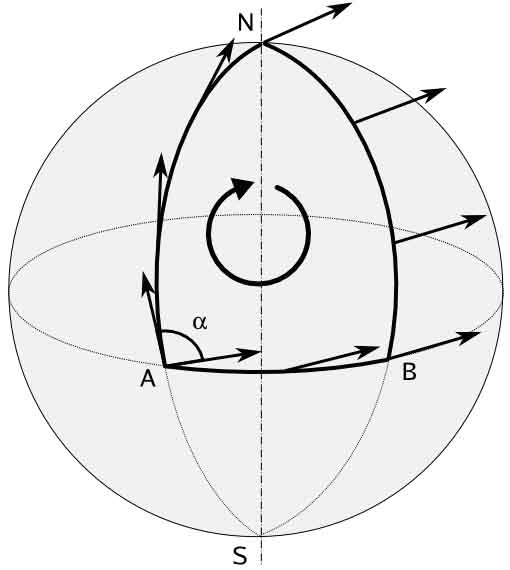
\includegraphics[width=3.5in]{image/barryphase.jpg}
          \caption{不完全过程}\label{pic_barryphase}
        \end{figure} 
        
        向量由N点经过B,A最后回到N, 整个过程中, 在三维空间中, 方向不变. 最后回到N点时,
        向量的方向发生了变化. 这个过程被称为不完全过程. 经历了一个过程, 最终回到初态的
        体系, 其状态可能会发生一个变化. 而上图变化和过程中, 某种程度上, 最后的结果提供了路径的
        曲率信息.

        于是我们产生这样一个疑问: 如果让一个量子系统绝热演化, 形成一个闭合回路, 也就是初态
        和末态的哈密顿量保持一致, 但是中途确实经历了一些变化. 最后初态和末态到底有什么差别?

        答案是显然的, 由绝热定理, 体系的初态和末态将只会相差一个常数相因子.   

        也即, 将前文所得的结果誊写一遍:
        \begin{equation}
          \begin{aligned}
            \psi(0) &= \varphi_k\\
            \psi(t_0) &= \varphi_k\mathrm{e}^{i\gamma_k(t_0)}\mathrm{e}^{i\theta_k(t_0)t_0}
          \end{aligned}  
        \end{equation}

        其中,
        \begin{equation}
          \begin{aligned}
            \theta_n(t_0) &= -\frac{1}{\hbar}\int_0^{t_0}E_n(t')\mathrm{d}t'\\
            \gamma_n(t_0) &= i\int_0^{t_0}\langle\varphi_n(t')|\varphi_n'(t')\rangle{}\mathrm{d}t'
          \end{aligned}
        \end{equation}

        上式中的动力学相因子$\theta_n(t_0)$显然是一个和时间有关, 或者说是和量子体系的态在其路径上的运动
        速度有关的. 这是一个及其糟糕的性质, 因为我们虽然可以控制体系处在绝对慢的绝热演化状态上, 却很难完全
        精确的操控其演化速度一直保持某个特定值上, 这样一来, 如果我想通过实验观测动力学相因子的变化,来验证我
        的某个量子猜想, 测量的误差有很大一部分来源于对体系操控的无能为力上. 这是一个令实验和理论物理学家们都
        头疼的预言. 

        于是我们转而去观察几何相因子, 期待他是不是会带来一些惊喜. 

        在一个闭合演化的\textbf{一维}量子体系中, 比如宽度周期性变化的一维无限深方势阱. 
        取一个周期为研究对象, 其几何相因子显然为:
        \begin{equation}
          \begin{aligned}
            \gamma_n(T) &=i\int_0^T\langle\varphi_n(t)|\dfrac{\partial}{\partial{}t}\varphi_n(t)\rangle\mathrm{d}t\\
                        &=i\int_0^T\langle\varphi_n|\dfrac{\partial{}R}{\partial{}t}\dfrac{\partial\varphi_n}{\partial{}R}\rangle\mathrm{d}t\\
                        &=i\int_0^T\langle\varphi_n|\dfrac{\partial\varphi_n}{\partial{}R}\rangle\dfrac{\partial{}R}{\partial{}t}\mathrm{d}t\\
                        &=i\int_a^a\langle\varphi_n|\dfrac{\partial\varphi_n}{\partial{}R}\rangle\mathrm{d}R\\
                        &=0
          \end{aligned}
        \end{equation}
        
        不得不说, 这个结果同样是令人沮丧的. 最终积分结果是什么都没有, 在一维情况下不可能求助于几何相因子了...

        那么三维情况下呢, 三维体系中的几何相又将是怎样的?
        \begin{equation}
          \label{barry_phase}
          \begin{aligned}
            \gamma_n(T) &=i\int_0^T\langle\varphi_n|\dfrac{\partial\varphi_n}{\partial{}R}\rangle\dfrac{\partial{}R}{\partial{}t}\mathrm{d}t\\
                        &\overset{3D}{=}i\oint_\mathbf{R}\langle\varphi_n|\dfrac{\partial\varphi_n}{\partial{}\vec{R}}\rangle\mathrm{d}\vec{R}\\
                        &=i\oint_\mathbf{R}\langle\varphi_n|\nabla_{\vec{R}}\varphi_n\rangle\mathrm{d}\vec{R}
          \end{aligned}
        \end{equation}
       
        这是一个振奋人心的结果, 因为在三维情况下, 虽然体系是封闭的积分, 但是这个积分一般不是零. 
        上式使用斯托克斯公式变换后, 这个结论或许可以看得更为清楚.    
        \begin{equation}
          \gamma_n(T) = i\int_s\nabla\times\langle\varphi_n(t)|\nabla\varphi_n\rangle\mathrm{d}\vec{s}
        \end{equation}
        
        式\eqref{barry_phase}中的相位显然是与量子体系在其路径上的演化速率无关的! 其值的大小, 只与路径上
        量子态的几何构型有关. 称, 该相位为Barry相.

       如果要使Barry相不是0, 一般需要满足以下几个条件:
        \begin{enumerate}[1.]
          \item 体系哈密顿量中含时参数多于一个.\footnote{一维谐振子Barry相就是0.}
          \item 体系哈密顿量有非平庸的复数解波函数.
          \footnote{若体系哈密顿量的本征波函数均为实函数, 
          则有$\langle\varphi_n(t)|\nabla\varphi_n\rangle = 0$}
        \end{enumerate}

      \subsubsection{Aharonov-Bohm效应\protect\footnote{本部分绝大多数观点来自\emph{格里菲斯电动力学 10.2.3}}}
        在经典电磁理论的基本定律(麦克斯韦方程组和洛伦兹公式)是不含势(磁矢势和电标势)的. 从逻辑上讲, 引入势的概念不过是数学上
        为了方便计算, 而在物理理论上是非必需的. 的确, 我们可以对势做所谓的'规范变换', 这种变换对场没有任何影响.

        然而, 在量子力学中, 势却有更重要的地位. 因为哈密顿量是用势, 而非电场和磁场强度来描述的.

        具体的:
        \begin{equation}
          \hat{H} = \dfrac{1}{2m}\left(\dfrac{\hbar}{i}\nabla-q\vec{A}\right)^2 + q\varphi
        \end{equation}
        
        更加致命的是, 在量子体系中, 即使是电场和磁场都是0的区域, 只要其势场不为0, 还是可能会引起一些物理效应. 这种效应由
        Aharonov和Bohm在1959年首先证明. 更精确地, 矢势可以影响带电粒子的量子行为, 即使它是在场本身为零的区域中运动.

        我们首先使用一个简单的例子来讨论所谓的\textbf{AB效应}.

        设想有一个无限长通电螺线管.

        \begin{figure}[H]
          \centering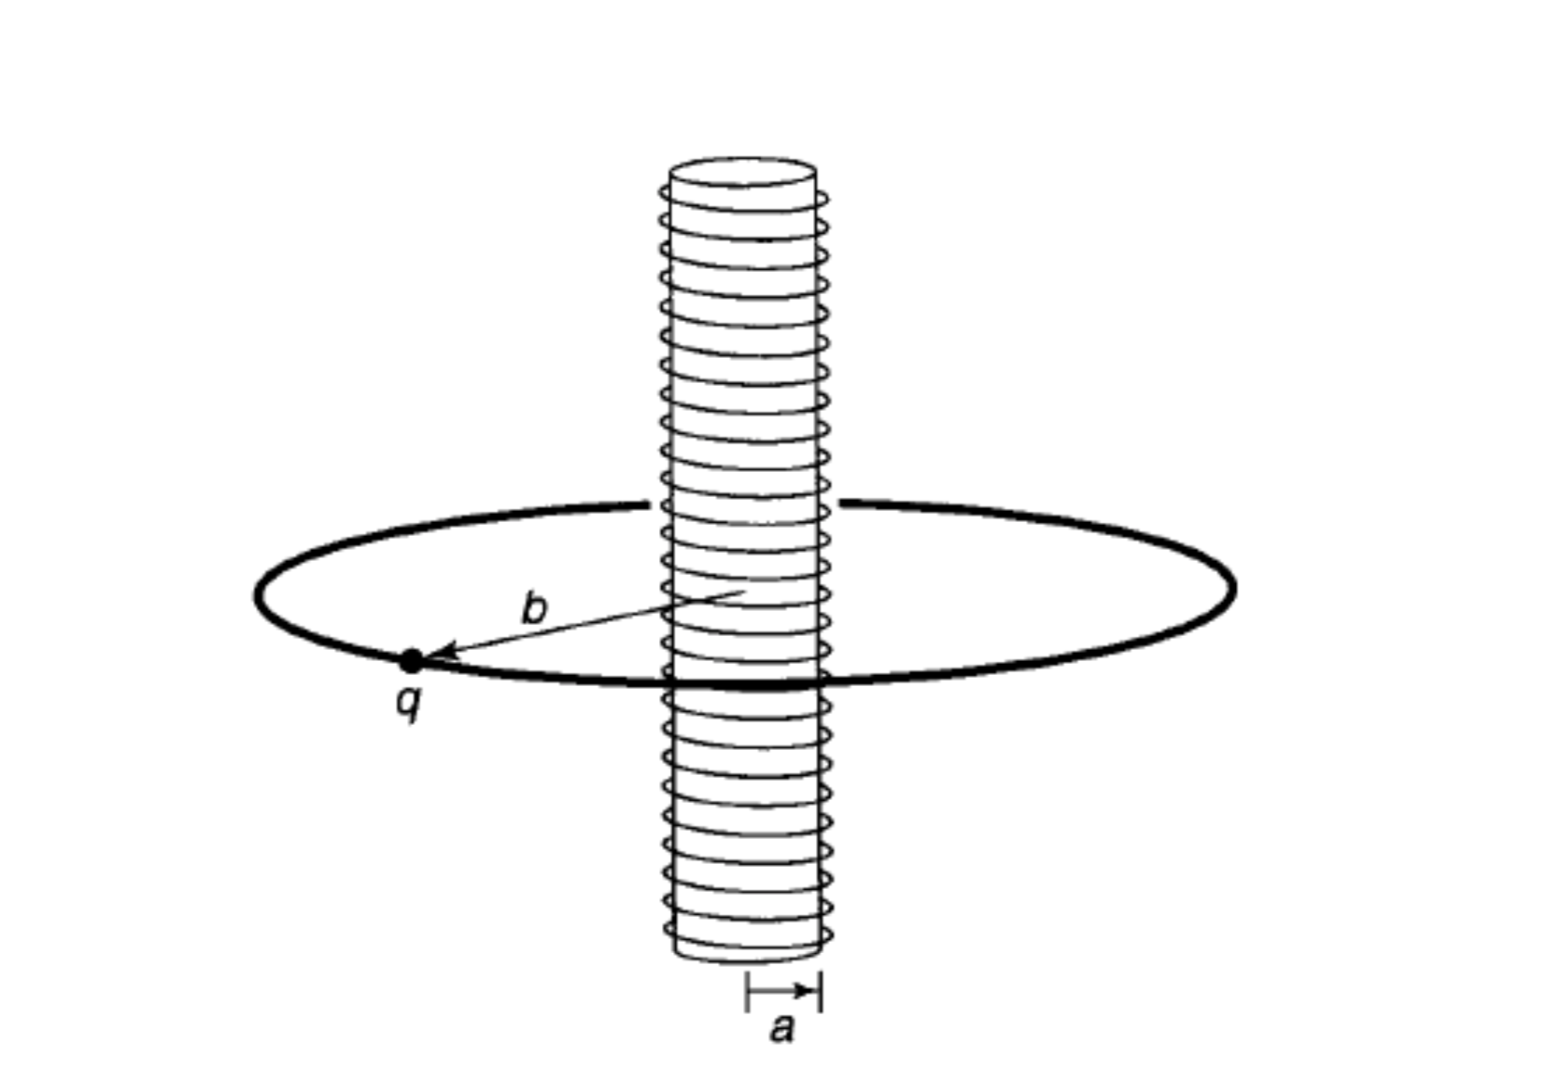
\includegraphics[width=3.5in]{image/ABeffect_1}
          \caption{理解AB效应的简单模型}\label{AB_effect_1} 
        \end{figure}
        
        假设一个粒子被限制在半径为b的圆环上运动. 螺线管通有稳恒电流I, 半径为a的螺线管沿轴向放置. 具体如Fig.%
        \ref{AB_effect_1}所示. 由于螺线管是无限长的, 因此其内部磁场是均匀的, 外部的磁场为零. 但在螺线管外部, 其
        矢势不为0. 如果采用库伦规范($\nabla\cdot\vec{A} = 0$), 螺线管外的磁矢势可以写作: 
        \begin{equation}
          \vec{A} = \frac{\Phi}{2\pi{}r}\hat{\phi}
        \end{equation}
        
        其中, $\Phi = \pi{}a^2B$是通过螺线管的磁通量. 螺线管自身不电,电标势为0. 因此有, 该体系的哈密顿量为:
        \begin{equation}  
          \label{hamilton_phi}
          H = \dfrac{1}{2m}\left[-\hbar^2\nabla^2+q^2A^2+2i\hbar{}q\vec{A}\cdot\nabla\right]
        \end{equation}

        注意到, 我们将粒子约束在了一个垂直于螺线管轴线方向的圆环上, 因此, 体系的状态波函数只与球坐标系中
        $\hat\phi$方向有关($r = b, \theta = \frac{\pi}{2}$). 

        因此有:
        \begin{equation}
          \label{nabla_phi}
          \nabla \to \dfrac{\mathrm{d}}{\mathrm{d}\phi}\dfrac{\hat\phi}{b}
        \end{equation}

        将\eqref{hamilton_phi}\eqref{nabla_phi}带入定态schr\"odinger方程可得:  
        \begin{equation}
          \dfrac{1}{2m}\left[-\dfrac{\hbar^2}{b^2}\dfrac{\mathrm{d}^2}{\mathrm{d}\phi^2}%
           + \left(\dfrac{q\Phi}{2\pi{}b}\right)^2+i\dfrac{\hbar{}q\Phi}{\pi{}b^2}%
          \dfrac{\mathrm{d}}{\mathrm{d}\phi}\right]\psi(\phi) = E\psi(\phi)
        \end{equation}
        
        对上式做一些简单的变形, 可得:
        \begin{equation}
          \begin{aligned}
            &\dfrac{\mathrm{d}^2\psi}{\mathrm{d}\phi^2} - 2i\beta\dfrac{\mathrm{d}\psi}{\mathrm{d}\phi}%
            +\varepsilon{}\psi = 0\\
            &\beta\equiv\dfrac{q\Phi}{2\pi\hbar}\\
            &\varepsilon\equiv\dfrac{2mb^2E}{\hbar^2}-\beta^2
          \end{aligned}
        \end{equation}

        求解上述方程可得如下结果:
        \begin{equation}
          \begin{aligned}
            \psi &= A\mathrm{e}^{i\lambda\phi}\\
            \lambda &= \beta\pm\sqrt{\beta^2+\varepsilon}\\
            &= \beta\pm\frac{b}{\hbar}\sqrt{2mE}
          \end{aligned}
        \end{equation}

        自变量$\phi$显然是满足自然边界条件的, 也即:
        \begin{equation}
          \label{nature_band}
          \psi(0) = \psi(2\pi{}n)
        \end{equation}

        因此, 将此边界条件带入, 求得波函数可得能量量子化形式为:
        \begin{equation}
          \beta\pm\frac{b}{\hbar}\sqrt{2mE} = n
        \end{equation}
        \begin{equation}
          E_n = \dfrac{\hbar^2}{2mb^2}\left(n-\frac{q\Phi}{2\pi\hbar}\right)^2, %
          \quad (n = 0,\pm1,\pm2,\pm3...)
        \end{equation}

        若不存在此螺线管, 则此体系的定态schr\"odinger方程可写作, 
        \begin{equation}
          -\dfrac{\hbar^2}{2mb^2}\dfrac{\mathrm{d}^2}{\mathrm{d}\phi^2}\psi(\phi) = E\psi(\phi)
        \end{equation}

        带入\eqref{nature_band}所示的自然边界条件, 可得:
        \begin{equation}
          E_n = \dfrac{\hbar^2}{2mb^2}n^2
        \end{equation}

        比较有无螺线管的两个能级, 可得到如下两个结论:
        \begin{enumerate}[*]
          \item 磁矢势对该物理体系的能量有影响, 影响体现在对量子数n的修正上.
          \item 螺线管使该量子体系的两重简并分裂: 正的n代表粒子运动方向与螺线管中电流方向一致;
                正的n比负的n有更低的能量(假设电荷为正), 负的n描述粒子的运动方向与螺线管中电流方向相反.
                更重要的是, 能量的允许值明显依赖螺线管内的场, 即便是粒子所处位置处的场为零!
                \footnote{引自: 格里菲斯量子力学10.2.3}
        \end{enumerate}

        下面考虑更一般的情况, 假设粒子在磁矢势$\vec{A}$不为零, 但其旋度$\nabla\times\vec{A} = 0$
        (也即磁场强度$B$为0)的区域运动. 其中磁矢势$\vec{A}$不随时间变化. 

        则其含时schr\"odinger方程可写作:
        \begin{equation}
          \label{1923_sch}
          \left[\dfrac{1}{2m}\left(\dfrac{\hbar}{i}\nabla-q\vec{A}\right)^2 + V\right]\psi%
          = i\hbar\dfrac{\partial\psi}{\partial{}t}
        \end{equation}

        其中, 如假定该磁场中不存在净电荷, 则势能$V$中不含电标势引起的势能$q\varphi$.

        为了进一步观察磁场对该体系影响, 对上述含时schr\"odinger方程做如下数学上的处理:

        令:
        \begin{equation}
          \label{1935_que}
          \begin{aligned}
            \psi &= \mathrm{e}^{ig}\Psi\\
            g(\vec{r}) &\equiv \dfrac{q}{\hbar}\int_{\vec{Q}}^{\vec{r}}\vec{A}(\vec{r'})%
                \cdot\mathrm{d}\vec{r'}
          \end{aligned}  
        \end{equation}

        $\vec{Q}$为任意选取的参考点, $\vec{Q}$的不同将只会引起量子态中一个常数相因子的差异. 另外, 
        只有在$\nabla\times\vec{A} = 0$的区域, 才可以定义$g$是$\vec{r}$的函数, 否则, 上述对磁矢势的积
        分将依赖于其具体的积分路径.

        将\eqref{1935_que}中的$\psi$带入\eqref{1923_sch}得:
        \begin{equation}
          -\dfrac{\hbar^2}{2m}\nabla^2\Psi + V\Psi = i\hbar\dfrac{\partial\Psi}{\partial{}t}          
        \end{equation}
        
        上述方程已完全与磁场无关, 因此, 可以得到这样的结论:

        \textbf{磁矢势对该体系量子态的影响, 完全体现在相因子$\mathbf{g(r)}$上!}

        为进一步理解AB效应产生的实际影响, 设想如下实验, 利用前文中所讨论过的螺线管体系, 一束电子束被分成
        两束, 分别通过螺线管的两侧, 最后再汇聚为一束. 

        上述实验具体图像如下所示:

        \begin{figure}[H]
          \centering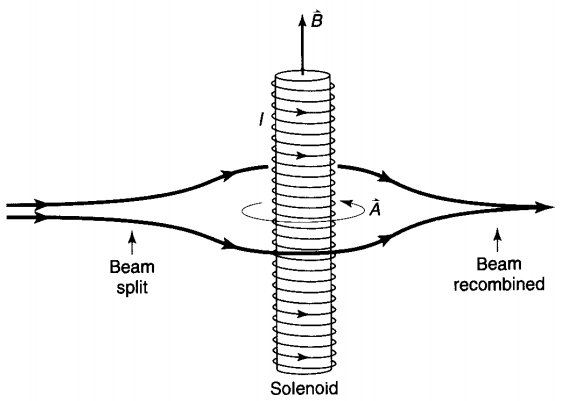
\includegraphics[width=3.5in]{image/ABeffect_2}
          \caption{AB效应}\label{AB_effect_2} 
        \end{figure}

        则, 由前文中的分析, 汇聚后的两束电子将有一个相位差, 进而产生干涉.

        具体的, 两束电子各自产生的相位差大小为:
        \begin{equation}
          \begin{aligned}
            g &= \dfrac{q}{\hbar}\int\vec{A}\cdot\mathrm{d}\vec{r} \\
              &= \dfrac{q\Phi}{2\pi\hbar}\int\dfrac{\hat{\phi}}{r}\cdot(r\hat{\phi}\mathrm{d}\phi)\\
              &= \pm\dfrac{q\Phi}{2\hbar}
          \end{aligned}
        \end{equation}
            
        进而, 两束电子间的相位差为:
        \begin{equation}
          \Delta{}g = \dfrac{q\Phi}{\hbar}
        \end{equation}

        这个相位差是已经被实验测得的了!\footnote{R.G.Cambers, Phys. Rev. Lett. \textbf{5}. 3(1960)}

        值得注意的是, AB效应和Barry相有着千丝万缕的联系.下面对这个问题做一些解释. 

        假设一个带电粒子被一个势$V(\vec{r}−\vec{R})$限制在一个箱子里(箱子的中心固定在螺线管外
        面一点$\vec{R}$). 具体的图像如下所示,

        \begin{figure}[H]
          \centering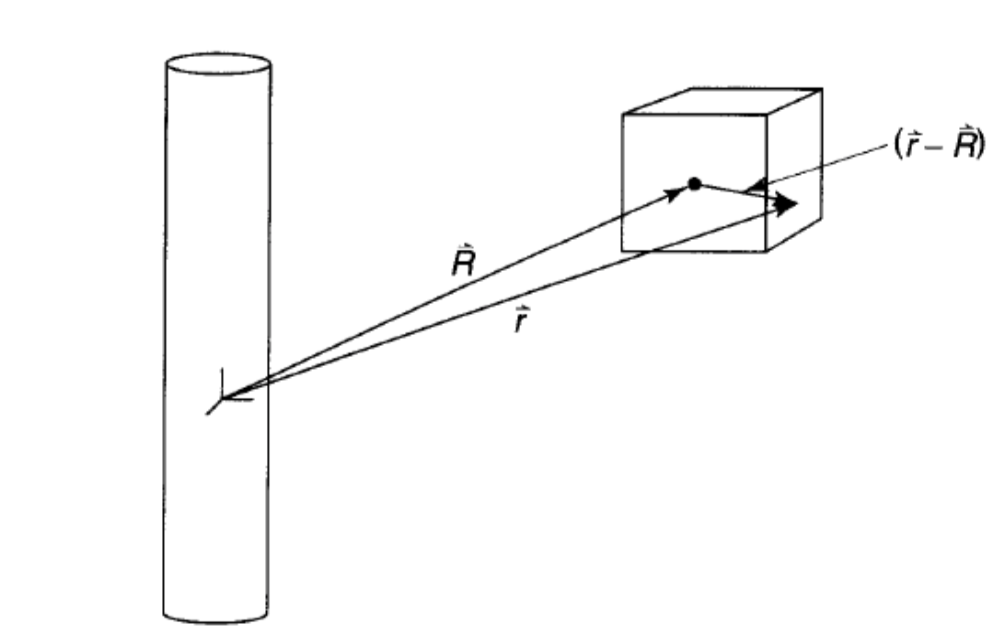
\includegraphics[width=3.5in]{image/Barry-ABeffect}
          \caption{AB效应与Barry相的联系}\label{AB_effect_Barry} 
        \end{figure}

        该体系的定态薛定谔方程为: 
        \begin{equation}
          \left\{\dfrac{1}{2m}\left[\dfrac{\hbar}{i}\nabla-q\vec{A}(\vec{r})\right]^2 + %
          V(\vec{r}-\vec{R})\right\}\psi_n = E_n\psi_n
        \end{equation}

        对上式采用之前的套路分离出磁矢势对体量子态的影响. 
        \begin{equation}
          \label{2009_psin}
          \begin{aligned}
            \psi_n &= \mathrm{e}^{ig}\Psi\\
                 g &\equiv \dfrac{q}{\hbar}\int_{\vec{R}}^{\vec{r}}\vec{A}(\vec{r'})%
                                           \cdot\mathrm{d}\vec{r'}
          \end{aligned}
        \end{equation}

        则$\Psi_n$应满足如下定态Schr\"odinger方程:
        \begin{equation}
          \left[\dfrac{\hbar^2}{2m}\nabla^2+V(\vec{r}-\vec{R})\right]\Psi_n = E_n\Psi_n
        \end{equation}

        注意到, $\Psi_n$只与在盒子中的相对位置有关, 也即, $\Psi_n$只是$\vec{r}-\vec{R}$这个整体的
        函数. 而$\psi_n$则是$\vec{r}$和$\vec{R}$两个独立变量的函数.

        现令螺线管, 以$R$定长绕着螺线管运动起来, 则此过程会产生所谓的Barry相.

        由\eqref{barry_phase}\eqref{2009_psin}, 可知, Barry相的大小为:
        \footnote{更细致的推导请参见: 格里菲斯量子力学 10.2.3末}
        \begin{equation}
          \begin{aligned}
           \gamma_n(T) &= i\oint_\mathbf{R}\langle\psi_n|\nabla_{\vec{R}}\psi_n\rangle\mathrm{d}\vec{R}\\
                       &= \dfrac{q}{\hbar}\oint\vec{A}(\vec{R})\cdot\mathrm{d}\vec{R}\\
                       &= \dfrac{q}{\hbar}\int_{\vec{S}}(\nabla\times\vec{A})\cdot\mathrm{d}\vec{S}\\
                       &= \dfrac{q\Phi}{\hbar}
          \end{aligned}
        \end{equation}

        由此可见, 上述AB效应引起的干涉相位和Barry相是相等的. 虽然量子体系所处的环境中磁场强度为0, 但
        体系最终的量子态仍然受到磁通量的影响.

   \section{定态散射理论}
      \subsection{一维散射问题}
        \subsubsection{一维散射问题的基本回顾}
          对于不含时的哈密顿量, 由定态薛定谔方程: 
          \begin{equation}
            \hat{H}\psi = E\psi
          \end{equation}
        
          若体系的能量E已知, 则可以解出体系的本征态, 其解的形式可以分为两类: 束缚态和扩展态. 所谓束缚态是指波函数
          在无穷远处为0的态, 所谓扩展态, 是指不含有束缚态特点的态.
          
          现设一束平面波在一维空间中运动, 遇到一高为$U_0$的势垒, 势垒的高度大于平面波的能量E. 此时, 平面波发生
          反射与透射, 形成所谓的散射态. 散射态属于扩展态的一种. 

          \begin{figure}
            \centering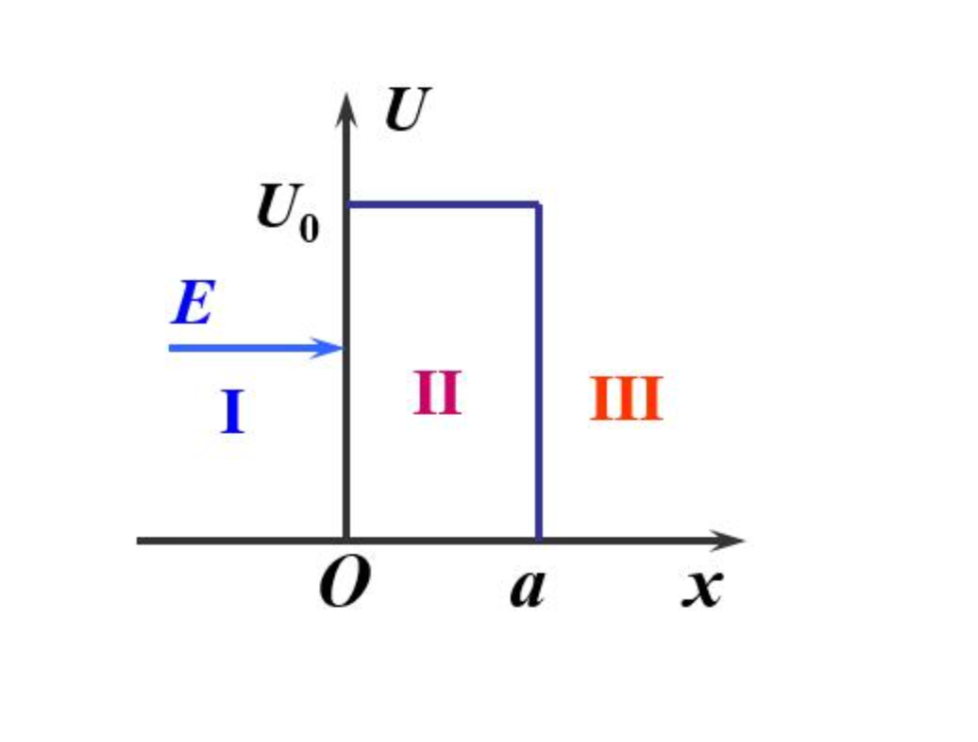
\includegraphics[width=3.5in]{image/scattering_state}
            \caption{一维散射问题}\label{1D_scatering} 
          \end{figure}

          其具体的波函数可有如下形式:
          \begin{equation}
            \begin{aligned}
              \psi_I(x) &= \mathrm{e}^{ikx} + r\mathrm{e}^{-ikx}\\
              \psi_{II}(x) &= A_2\mathrm{e}^{\alpha{}x}+B_2\mathrm{e}^{-\alpha{}x}\\
              \psi_{III}(x) &= t\mathrm{e}^{ikx}
            \end{aligned}
          \end{equation}
          
          求解此量子体系, 实际上就是要求解上述$r,t,A_2,B_2$四个系数.

          为了更加形象的研究该量子体系, 引入所谓的反射系数R和透射系数T:
          \begin{equation}
            \begin{aligned}
              T &= \frac{J_t}{J_i}\\
              R &= \frac{J_r}{J_i}            
            \end{aligned}
          \end{equation}
           
          其中, 
          \begin{equation}
            \label{J_function}
            J = \frac{1}{2m}\left[\psi^{*}\hat{P}\psi-\psi\hat{P}\psi^{*}\right]    
          \end{equation}


          上式中的$J$被称为概率流密度, 在一维问题中, 其可理解为单位时间流过某一一维截面的概率大小.

          下面简单的给出几个典型散射态模型的解:

          \textbf{1.普通方式垒}
          \begin{equation}
            T(E) = \dfrac{1}{1+\dfrac{\sinh^2(\alpha{}a)}{\dfrac{E}{V}\left(1+\dfrac{E}{V}\right)}}
          \end{equation}
          
          \textbf{2. 半壁无限高有限深方势阱}
          \begin{equation}
            T(E) = \dfrac{1}{1+\dfrac{\sin^2(k'a)}{\dfrac{E}{V}\left(1+\dfrac{E}{V}\right)}}
          \end{equation}
          
          \textbf{3. 量子共振隧穿}
            \begin{equation}
              ka = n\pi{}T = 1
            \end{equation}

        \subsubsection{计算一维散射问题的一般方法}
          下面引入一种计算散射态问题的一般方法, 也就是所谓的``传递矩阵方法''. 如 Fig.\ref{1D_scatering}所示,
          注意到这样一个事实, 此量子态的散射的特性只由粒子本身的能量以及最初的区域和最末的区域的系数和势能决定.
          在上述的参数中, 只有系数't','r'是未知的. 因此求解此散射态问题就化为了求解最初区域和最末区域波函数
          系数的问题. 
          
          首先关注I区与II区, 在O点处满足条件:
          \begin{equation}
            \begin{aligned}
              \psi_I(0) &= \psi_{II}(0)\\
              \psi_I'(0) &= \psi_{II}(0) 
            \end{aligned}
          \end{equation}

          由波函数在I,II区的具体形式, 可得:
          \begin{equation}
            \begin{aligned}
              \mathrm{e}^{ik\cdot0} + \mathrm{e}^{-ik\cdot0} &= %
                      A_2\mathrm{e}^{\alpha\cdot0} + B_2\mathrm{e}^{-\alpha\cdot0}\\
              ik(\mathrm{e}^{ik\cdot0} - \mathrm{e}^{-ik\cdot0}) &= %
                      \alpha(A_2\mathrm{e}^{\alpha\cdot0} - B_2\mathrm{e}^{-\alpha\cdot0})
            \end{aligned}
          \end{equation}
          
          进而, 上式可以化为:
          \begin{equation}
            \left(\begin{array}{c}A_2\\B_2\end{array} \right) = %
            T_1\left(\begin{array}{c}1\\r\end{array} \right)%
          \end{equation}
          
          同样利用II,III边界的条件, 可以得到:
          \begin{equation}
            \left(\begin{array}{c}t\\0\end{array} \right) = %
            T_2\left(\begin{array}{c}A_2\\B_2\end{array}\right) = %
            T_2T_1\left(\begin{array}{c}1\\r\end{array}\right) = %
            T\left(\begin{array}{c}1\\r\end{array}\right)
          \end{equation}

          上述方法可以推广到多势垒甚至是连续变化势垒\footnote{如抛物线形势垒}的情况, 对于连续势垒只需要将其近似化为
          多个矩形势垒即可. 利用不同矩形势垒之间的边界条件, 就可以得到不同区域参数间的转移矩阵, 最终, 可将最初区域的
          系数和最末区域的系数利用所有的转移矩阵连接起来, 构成如下形式:
          \begin{equation}
          \left(\begin{array}{c}t\\0\end{array} \right) = %
          T_N{}T_{N-1}\ldots{}T_1\left(\begin{array}{c}1\\r\end{array}\right) \equiv%
          T\left(\begin{array}{c}1\\r\end{array}\right)
          \end{equation} 

          进而, 就可以解出我们所关心的系数, $r$与$t$ !

      \subsection{三维散射问题}
        \subsubsection{碰撞过程和散射截面}
          对散射问题较为确切的物理描述为:\textbf{具有一定动量(能量)的入射粒子沿着确定的方向射向靶粒子,由于受
          到靶粒子的作用(在空间小区域内)而发生了偏转, 沿某一方向射出.}

          散射可分为两类: 弹性散射和非弹性散射. 其中弹性散射是靶粒子和入射粒子内部结构均不发生变化的散射过程. 
          而第二种散射模式则会牵扯到核反应, 过程较为复杂. 这里, 我们所研究的三维散射问题均为弹性散射. 

          为描述三维散射问题的特征, 引入微分散射截面的概念:
             
          首先, 下面的公式应该是好理解的:
          \begin{equation}
          \label{q_scattering}
            \mathrm{d}N = q(\theta, \varphi)J_i\mathrm{d}\Omega
          \end{equation}
          
          其中, $\mathrm{d}N$是单位时间内穿过dS的粒子数, $\mathrm{d}\Omega$是某一散射方向的立体角, 
          $J_i$是入射粒子流密度(单位时间内通过单位横截面积的粒子数). $q(\theta, \varphi)$是与散射方向有关的
          系数. 具体的细节如 Fig.\ref{3D_scatering} 所示.

          \begin{figure}
            \centering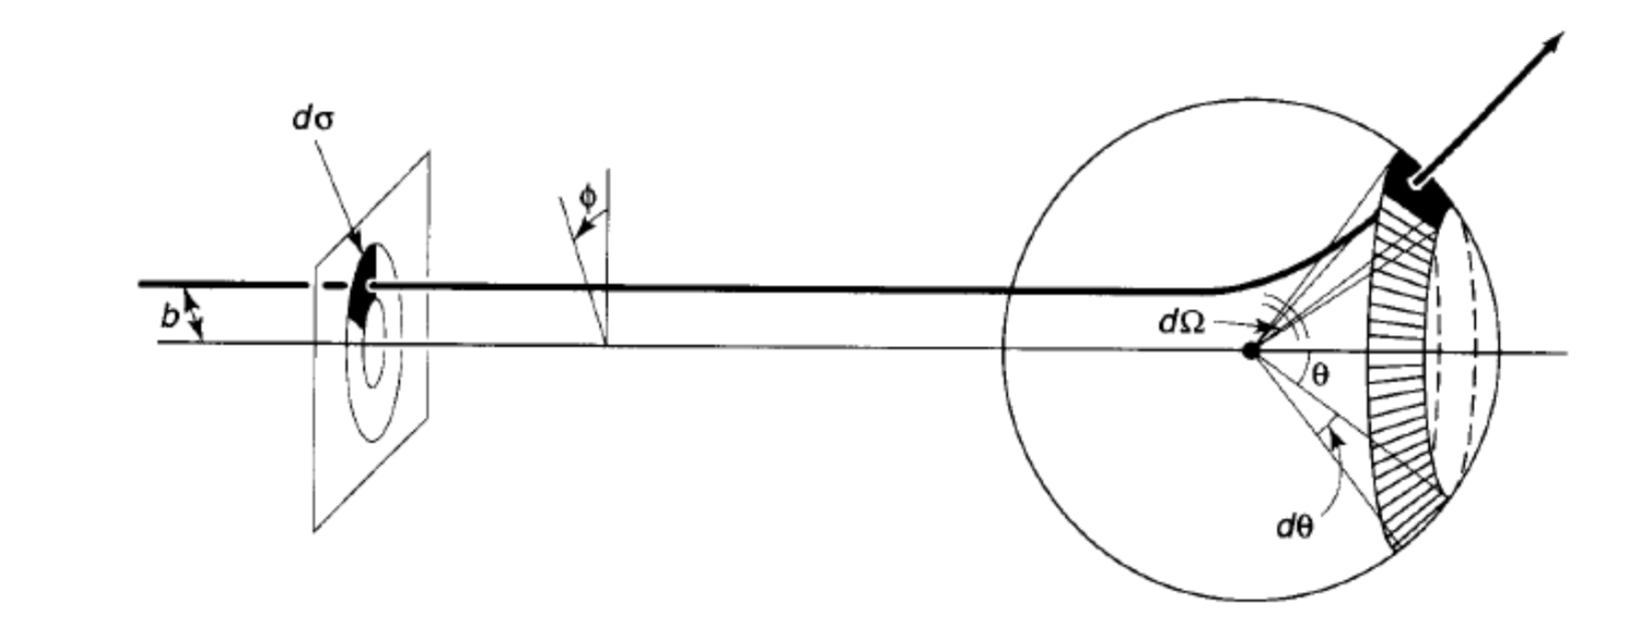
\includegraphics[width=3.5in]{image/3D_scattering_pic}
            \caption{三维散射问题}\label{3D_scatering} 
          \end{figure}

          \eqref{q_scattering}可以化为如下两种形式:
          \begin{equation}
            \begin{aligned}
              q(\theta, \varphi) &= \frac{\mathrm{d}N}{J_i}\cdot\frac{1}{\mathrm{d}\Omega}\\
              q(\theta, \varphi)J_i &= \frac{\mathrm{d}N}{\mathrm{d}\Omega}\\
            \end{aligned}
          \end{equation}

          对上述两个式子可以分别有如下理解:
          \begin{enumerate}[*]
            \item 单位面积的入射粒子在某一散射方向上的散射几率, 所谓的某方向的散射粒子数, 实际是在这一方向
            上的一个单位立体角内的粒子总数.
            \item 若某一组入射粒子被从$(\theta, \varphi)$方向散射, 那么他必然来源于入射粒子束截面的某一特殊区域上. 
            这一区域总体的有效面积为$q(\theta, \varphi)$.
          \end{enumerate}
        
          因此, 对$q(\theta, \varphi)$有如下两种称呼: 角分布和微分散射截面.
          
          特殊的, 由微分散射截面的定义, 可以得到总的散射截面:
          \begin{equation}
            Q = \int_{\Omega}q(\theta, \varphi) \sin(\theta)\mathrm{d}\theta\mathrm{\varphi}
          \end{equation}
          
          Q是对全立体角积分, 也就是对所有的可能的散射方向的积分.
          
          若此散射势与方向$\varphi$无关, 则上述公式就可以化为:
          \begin{equation}
            Q = 2\pi\int_0^{\pi}q(\theta, \varphi)\sin(\theta)\mathrm{d}\theta
          \end{equation}

          最终Q的物理意义就是:入射粒子束中只有一个特殊区域中的粒子可以被靶粒子散射, 这个区域的有效面积为Q. 

          为了更具体的理解散射截面这一概念, 下面引入一个具体的例子. 

          \begin{figure}
            \centering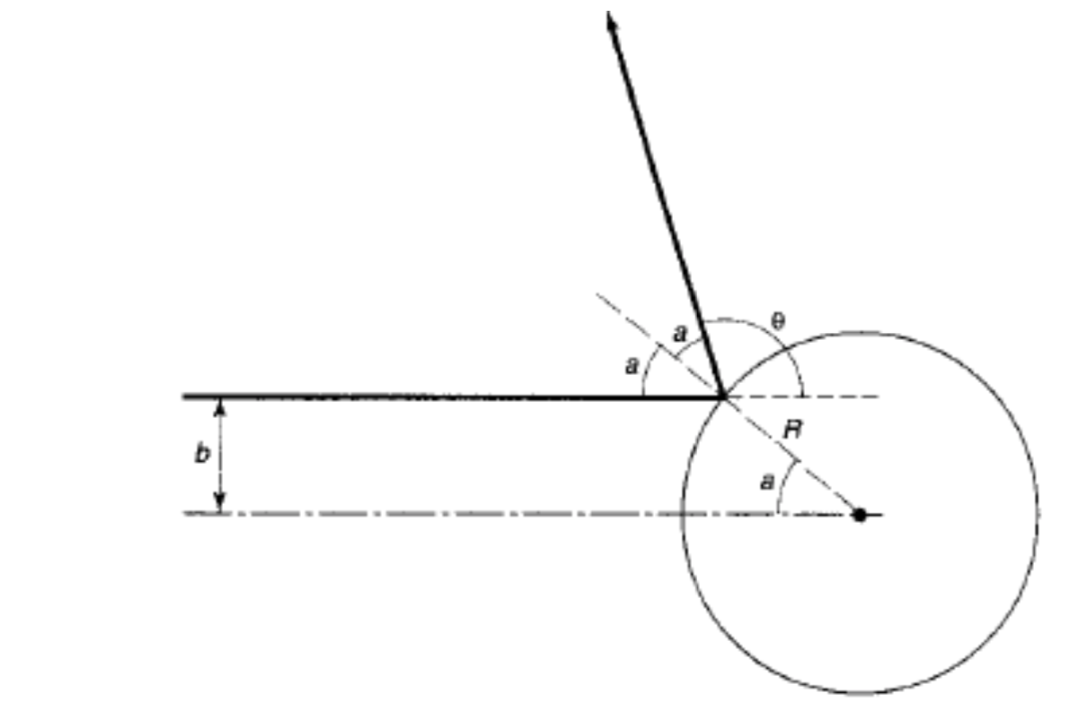
\includegraphics[width=3.5in]{image/iron_ball_model}
            \caption{钢球模型}\label{iron_ball_model} 
          \end{figure}
          
          设想有一个经典的钢球, 入射粒子由远处射向铁球, 铁球的半径为$R$, 则此体系的总散射截面显然为$\pi^2R$.
          \footnote{太阳光照射在这个球上, 会形成一个影子, 这个影子大小恰好为$\pi{}R^2$.}
          下面利用之前的微分散射截面积分的形式来计算出这一结果. 

          注意到这样一个事实, 总的散射截面实际上一个圆, 在此的内部每一个同心圆都对应一个散射方向$\theta$, 
          且微分散射截面应与$\varphi$方向无关. 因此, 在某一特殊方向$(\theta, \varphi)$上散射的粒子数为:
          \begin{equation}
            \begin{aligned}
              \mathrm{d}N &= J_i * b\mathrm{d}\varphi * \mathrm{d}b\\
              b &= R\sin(\frac{\pi-\theta}{2})\\
                &= R\cos(\frac{\theta}{2})
            \end{aligned}
          \end{equation}

          因此, 可以解出, 微分散射截面为:
          \begin{equation}
            q(\theta, \varphi) = \frac{R^2}{4}
          \end{equation}

          进而, 总的微分散射截面: 
          \begin{equation}
            \begin{aligned}
              \mathrm{d}N &= J_i * b\mathrm{d}\varphi * \mathrm{d}b\\
              Q &= 2\pi\int_0^{\pi}\frac{R^2}{4}\sin(\theta)\mathrm{d}\theta\\
              &= \pi{}R^2    
            \end{aligned}
          \end{equation}

          这与我们之前得到的结论是一致的. 
          \ \\

          \textbf{下面对量子力学中的散射问题做简要阐述:}

          散射现象涉及A, B两个物体, 在质心系下两体问题化为单体问题, 又考虑到入射粒子质量一般远远小于
          靶粒子. 因此, 此问题的的解可视为是以靶粒子为中心的中心势场对入射粒子产生的影响. 

          为求解这一影响, 首先列出入射粒子的schr\"odinger方程:
          \begin{equation}
            -\frac{\hbar^2}{2m} \nabla^2\psi + U(\vec{r})\psi = E\psi
          \end{equation}

          在$r\to\infty$时, $U(\vec{r})\to0$, 此时, 无穷远处的波函数可以视为两类波函数的叠加:
          一个是入射平面波的波函数, 一个是反射球面波的波函数. 因此, 在无穷远处波函数的形式可以写为:
          \begin{equation}
            \begin{aligned}
              \psi(\vec{r}) &= \mathrm{e}^{ikz} + f(\theta)\dfrac{\mathrm{e}^{ikr}}{r} \\
              k &\equiv \frac{\sqrt{2mE}}{\hbar}
            \end{aligned}
          \end{equation}

          \begin{figure}
            \centering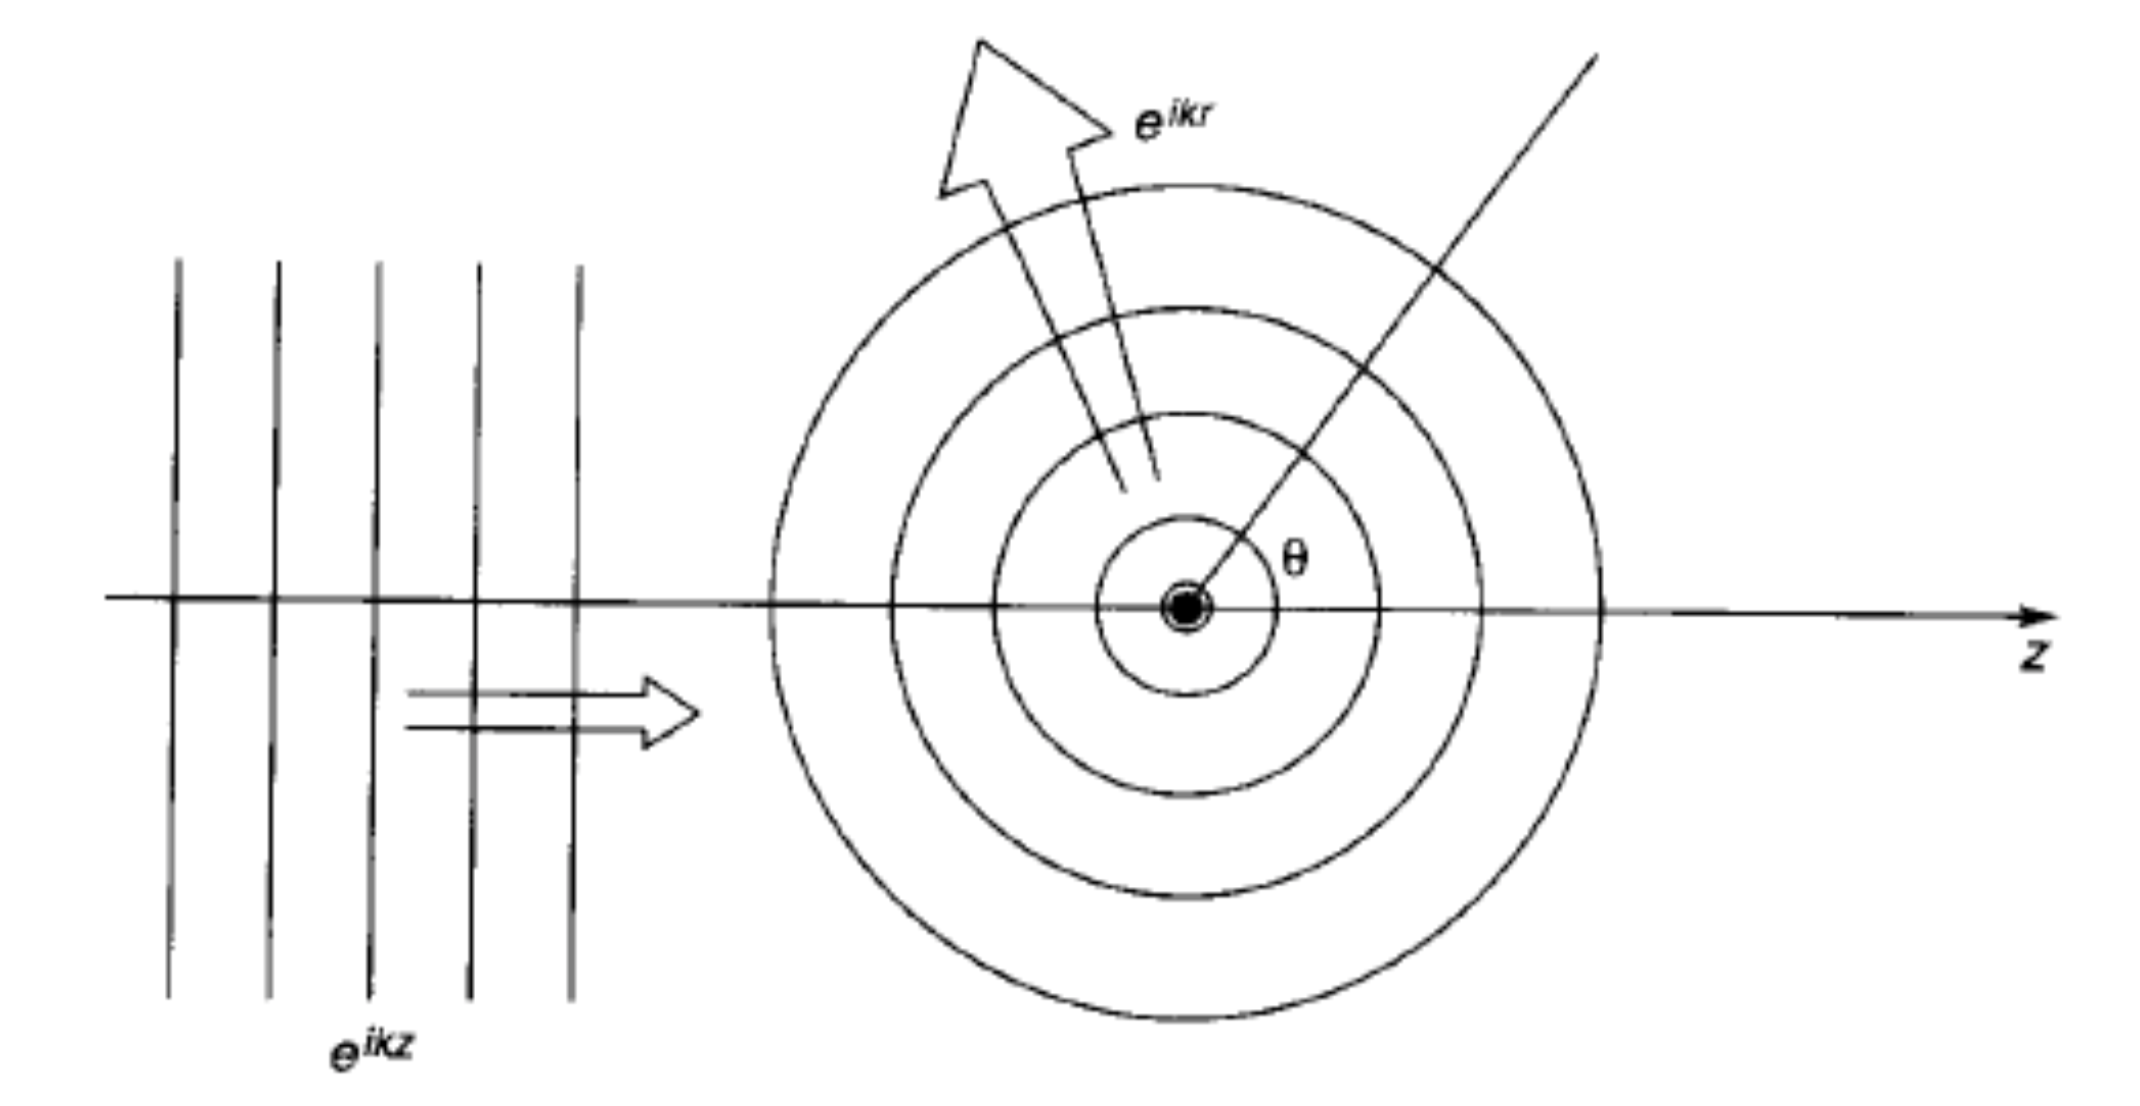
\includegraphics[width=3.5in]{image/quantum_scatterting_psi}
            \caption{散射波函数形式的确定}\label{quantum_scatterting_psi} 
          \end{figure}

          这里, 散射波有$\frac{1}{r}$因子的原因是: 要保持概率在不同球面上的几率守恒.
          
          考虑之前引入的流密度的公式\eqref{J_function}
          \begin{equation}   
            J = \frac{1}{2m}\left[\psi^{*}\hat{P}\psi-\psi\hat{P}\psi^{*}\right]    
          \end{equation}

          将入射波波函数与反射波波函数分别带入上式中, 可得到如下两个结论
          \begin{equation}
            \begin{aligned}
              J_z &= \frac{k\hbar}{m} = v\\
              J_{\vec{r}} &= \frac{k\hbar}{m}\frac{|f(\theta)|^2}{r^2}\\
                          &= v\frac{|f(\theta)|^2}{r^2}
            \end{aligned}
          \end{equation}

          则单位面积上散射的粒子数为:
          \begin{equation}
            \begin{aligned}
              \mathrm{d}N &= J_r\mathrm{d}S \\
                          &= v|f(\theta)|^2\frac{\mathrm{d}S}{r^2}\\
                          &= v|f(\theta)|^2\mathrm{d}\Omega
            \end{aligned}
          \end{equation}

          由微分散射截面的定义式, 可知:
          \begin{equation}
            \label{fandq}
            q(\theta) = \frac{\mathrm{d}N}{J_z\mathrm{d}\Omega} = |f(\theta)|^2
          \end{equation}

          由此可见, $f(\theta)$的地位在散射特性中尤其重要. 

          于是, 在量子力学体系下求解三维散射问题最终就可以化为:
          求解下列能量已知的, 满足散射边界条件定态Schr\"odinger方程. 
          \begin{equation}
            \label{3.2.1:corequestion}
            \left\{
              \begin{array}{l}
              \left[-\dfrac{\hbar^2}{2m}\nabla^2+V(r)\right]\psi(\vec{r}) = E\psi(\vec{r})\\ \ \\
              \psi(\vec{r}) \overset{r\to\infty}{\longrightarrow}\mathrm{e}^{ikz} + f(\theta)\dfrac{\mathrm{e}^{i\vec{k}\vec{r}}}{r}
              \end{array} \right. 
          \end{equation}
 
          上述方程的严格求解是困难的.
          
          因此, 不得不采用一些近似方法. 

          下面将介绍两种常见的近似方法: 分波法 和 Born近似法. 
        
        \subsubsection{分波法}
          分波法的思想来源于这样一个事实: 在中心力场下, 力学量\{$\hat{H}, \hat{L}^2, \hat{L}_z$\}为守恒量, 
          也就是他们都满足与体系的哈密顿量对易这一条件\footnote{艾伦菲斯特定理}, 但是动量算符在此体系中却不是守恒量.
          这一点是显然的, 因为有$[P,H]\ne0$. 

          然而实际上, 体系的入射波$\psi_0 = \mathrm{e}^{ikz}$却是动量$(0,0,\hbar{}k)$的本征态.
          因此, 在接受中心势场散射过程中, 若直接以这种
          动量本征态的入射波形式进行运算, 计算上将是困难的.同时, 又考虑到球谐函数$Y_{lm}$是中心势场问题中守恒量
          \{$\hat{L}^2, \hat{L}_z$\}的共本态.于是, 采用将入射波分解为球谐函数的思想求解此问题.
          
          有,
          \begin{equation}
            \mathrm{e}^{ikz} = \mathrm{e}^{ikr\cos\theta} = %
            \sum_{l=0}\sqrt{4\pi(2l+1)}i^lj_l(kr)Y_{l0}(\theta)
          \end{equation}

          进而, $\psi$就可以写成:  
          \begin{equation}
            \label{fbf:1}
            \begin{aligned}
              \lim_{r\to\infty}\psi(\vec{r}) &= \sum_{l=0}\left[%
              \sqrt{4\pi(2l+1)}i^lj_l(kr)Y_{l0}(\theta)+f_l(\theta)\dfrac{e^{ikr}}{r}\right]\\
              &= \sum_{l=0}\left[\sqrt{4\pi(2l+1)}i^l\dfrac{\mathrm{e}^{i(kr-\frac{\pi{}l}{2})}%
              -\mathrm{e}^{-i(kr-\frac{\pi{}l}{2})}}{2ikr}Y_{l0}(\theta)+f_l(\theta)%
              \dfrac{e^{ikr}}{r}\right]
            \end{aligned}
          \end{equation}

          上式中的$f_l(\theta)$是某一个分波(球谐函数)所产生的反射波的振幅. 下面的关系式是显然的:
          \begin{equation}
            \label{fbf:3}
            f(\theta) = \sum_{l}f_l(\theta)
          \end{equation}

          下面从另一个角度考虑这个问题:

          中心力场的波函数的一般表达式为:
          \begin{equation}
            \psi = \sum_l R_l(kr)Y_{l0}(\theta)
          \end{equation}

          球谐函数$Y_{l0}$为已知的函数, 主要求解的是$R$函数的形式.
          将上式带入Schr\"odinger方程
          \begin{equation}
            \label{fbf:2}
            \left[-\dfrac{-\hbar^2}{2m}\nabla^2+V(\vec{r})\right]\psi(\vec{r}) = E\psi(\vec{r})
          \end{equation}

          方程可化为:
          \begin{equation}
            \left[-\dfrac{\hbar^2}{2m}\dfrac{\mathrm{d}^2}{\mathrm{d}r^2}+%
            V(\vec{r})+ \dfrac{l(l+1)\hbar^2}{2mr^2}\right]u(r) = Eu(r)
          \end{equation}
          
          其中, $u(r) = r\cdot{}R(r)$

          上述方程关于$u$的解是我们所熟悉的广义拉盖尔多项式.
          
          然而, 在散射问题中, 通过物理意义上的分析, 球谐函数在接受中心势场散射时形式不变,  
          同时, 分波径向波函数在无穷远处可以写成如下形式:
          \begin{equation}
            \begin{aligned}
              \lim_{r\to\infty}R(kr) &= %
              \sqrt{4\pi(2l+1)}i^l\left[j_l(kr)+\dfrac{a_l}{2}h_l(k)\right]\\
              &= \sqrt{4\pi(2l+1)}i^l\left[(1+a_l)\mathrm{e}^{i(kr-\frac{l\pi}{2})}-%
                       \mathrm{e}^{-i(kr-\frac{l\pi}{2})}\right]\cdot\frac{1}{2ikr}
            \end{aligned}
          \end{equation}

          这与广义拉盖尔多项式的精确解是不矛盾的. 

          对于一个确定的分波, 在弹性散射后和弹性散射前, 应满足几率守恒. 更具体地, 由\eqref{fbf:1}, 有:  
          \begin{equation}
            \begin{aligned}
              \left|(1+a_l)\mathrm{e}^{i(kr-\frac{l\pi}{2})}-\mathrm{e}^{-i(kr-\frac{l\pi}{2})}\right|^2 &= %
              \left|\mathrm{e}^{i(kr-\frac{l\pi}{2})}-\mathrm{e}^{-i(kr-\frac{l\pi}{2})}\right|^2\\
              |1+a_l| &= 1\\
              1 + a_l &= \mathrm{e}^{2i\eta_l}\\
              a_l &= \mathrm{e}^{i\eta_l}2i\sin\eta_l 
            \end{aligned}
          \end{equation}
           
          上述四式是等价的. 

          将上述关于$a_l$的表达式带回到原波函数, 可得:  
          \begin{equation}
              \lim_{r\to\infty}R(kr) = %
              \sqrt{4\pi(2l+1)}i^l\mathrm{e}^{i\eta_l}sin(kr-\frac{\pi{}l}{2}+\eta_l)\cdot\frac{1}{kr}
          \end{equation}

          对比上述径向波函数形式与未被散射前分波波函数\eqref{fbf:1}的形式, 显然, 散射后的径向波函数只改变了一个正弦函数中的
          相位$\eta_l$. 将上述波函数的形式再回带到之前所得到的径向波函数方程\eqref{fbf:2}中, 可得到相移$\eta_l$的具体数值.

          \textbf{至此, 散射问题在无穷远处的行为. 下面求解其散射截面的形式.}

          对于第$l$分波的散射波, 其形式为:
          \begin{equation}
            \begin{aligned}
              &\lim_{r\to\infty}f_l(\theta)\dfrac{\mathrm{e}^{ikr}}{r}\\
              &=\lim_{r\to\infty}\left[\sqrt{4\pi(2l+1)}i^l\dfrac{a_l}{2}h_l(k)Y_{l0}\right]\\
              &= \sqrt{4\pi(2l+1)}i^l\dfrac{a_l}{2ikr}\mathrm{e}^{i(kr-\frac{\pi{}l}{2})}Y_{l0} \\
              &= \sqrt{4\pi(2l+1)}i^l\dfrac{\mathrm{e}^{i\eta_l}\sin\eta_l}{kr}\mathrm{e}^{i(kr-\frac{\pi{}l}{2})}Y_{l0} \\
              &= \sqrt{4\pi(2l+1)}\mathrm{e}^{i\eta_l}\sin\eta_lY_{l0}\dfrac{\mathrm{e}^{ikr}}{kr} \\ 
            \end{aligned}
          \end{equation}

          从而,
          \begin{equation}
            f_l(\theta) = \dfrac{\sqrt{4\pi(2l+1)}}{k}\mathrm{e}^{i\eta_l}\sin\eta_lY_{l0}
          \end{equation}

          进而, 由\eqref{fbf:3}, 可得:
          \begin{equation}
            f(\theta) = \sum_lf_l(\theta) %
            = \sum_l\dfrac{\sqrt{4\pi(2l+1)}}{k}\mathrm{e}^{i\eta_l}\sin\eta_lY_{l0}
          \end{equation}

          由\eqref{fandq}, 微分散射截面可写为:
          \begin{equation}
            q(\theta) = |f(\theta)|^2 = \dfrac{4\pi}{k}%
             \left|\sum_l\sqrt{2l+1}\mathrm{e}^{i\eta_l}\sin\eta_lY_{l0}\right|^2
          \end{equation}

          总散射截面\footnote{$q$中只有球谐函数与$\Omega$有关, 其积分为1.}为:
          \begin{equation} 
            \label{zssjm}
            Q = \int\mathrm{d}\Omega\left|f(\theta)\right|^2 %
              = \dfrac{4\pi}{k^2}\sum_l(2l+1)\sin^2\eta_l
          \end{equation}

          \textbf{至此, 我们求出了散射问题所有基本参量, 下面讨论四个与散射相关的问题.}

          \textbf{1. 相移的正负与势能正负的关系}
            
            由简单的对比和物理图像上的理解, 就可以得到如下结论: 相移的符号与势场符号相反. 也就是, 中心力场为排斥力 
            则相移为负值, 中心力场为吸引力时相移为正.

          \textbf{2. 分波法的适用条件}
            
          首先给出结论:
          \textbf{分波法适用于短力程的低能散射, 这里的低能是入射粒子相对与靶粒子低能.}

          由之前的描述, 可以知道, 分波法的精髓, 实际上就是把动量本征态---沿z方向传播的平面波, 分解
          为角动量平方和角动量z分量共本态---球谐函数. 
          
          原则上讲, 分波法是个严格的处理方法, 但实际应用中, 我们不可能计算所有分波的贡献. 
          如果$f(\theta)$表达式中级数收敛的很快, 只需要计算前面几个分波即可. 因此, 如何确定该保留多少分波, 就成为
          一个亟待解决的问题. 

          注意到, 不同的分波实际上代表粒子不同的角动量. 若使用半经典理论分析此问题, 则结论将是显然的. 

          对于一个相互作用力力程为$a$的散射体系,入射粒子的速度为$v$, 质量为$m$, 则该粒子能拥有的最大角动量为$mva$
          \footnote{粒子入射方向所在直线与靶粒子的距离, 也就是所谓的瞄准距离, 最大为a}. 

          因此, 角动量量子数最大值
          \begin{equation}
            \label{fbftj}
            l_{max} \approx \dfrac{mva}{\hbar} = \sqrt{\dfrac{2mE}{\hbar^2}}a
          \end{equation}

          由此, 分波法分波只需在$l_{max}$处截断即可.

          为了更直观的理解这一截断方法, 举两个例子:

          \emph{1. 核子-核子散射}
          \begin{equation}
            \begin{aligned}
              a &\approx 10^{-15}m\\
              m &= \dfrac{938MeV}{c^2}\\
              \hbar &= 6.58\times10^{-22}MeV\cdot{}s\\
              l_{max} &\approx \dfrac{\sqrt{E(MeV)}}{4.5}
            \end{aligned}
          \end{equation}

          \emph{对于能量小于$20MeV$的散射, 只考虑S波与P波即可.}

          \emph{2. 电子-原子核散射}
          \begin{equation}
            \begin{aligned}
              a &\approx 0.53\times10^{-10}m\\
              m &= \dfrac{0.511MeV}{c^2}\\
              \hbar &= 6.58\times10^{-22}MeV\cdot{}s\\
              l_{max} &\approx 267\sqrt{E(MeV)}
            \end{aligned}
          \end{equation}
            
          \emph{对于能量小于$1MeV$的散射, 仅考虑S波即可.}

          \textbf{3. 光学定理}
          
          总的散射截面和向前散射振幅有关系:
          \begin{equation}
            Q = \dfrac{4\pi}{k}\mathrm{Im}f(0)
          \end{equation}

          这个关系是显然的, 只要注意到球谐函数有性质:
          \begin{equation*}
            Y_{l0}|_{\theta = 0} = \sqrt{\dfrac{2l+1}{4\pi}}
          \end{equation*}

          即可. 

          \textbf{4. 量子钢球散射}

          前文中, 我们讨论了所谓的经典钢球的散射截面, 下面来讨论量子钢球模型.

          所谓量子钢球模型, 实际上是势场形式为:
          \begin{equation}
            V(r) = \left\{
            \begin{array}{rl}
              \infty, & r<R\\
              0, & r\geq{}R
            \end{array}\right.
          \end{equation}

          的中心势场散射. 

          设该散射为低能散射, 仅考虑S波. 则有$Y_{00} = 1$, 进而, 与径向波函数相关联的$u$的形式解为:
          \begin{equation}
            \left\{
            \begin{array}{ll}
              u_0(r) = 0, & r < R \\
              u_0(r) = A\sin(kr+\eta_0), & r\geq{}R
            \end{array}\right.
          \end{equation}

          利用$R$处的连接条件, 可得:
          \begin{equation*}
            A\sin(kR+\eta_0) = 0
          \end{equation*}

          从而, 
          \begin{equation}
            \eta_0 = -kR
          \end{equation}

          总的散射截面:
          \begin{equation}
            Q = \dfrac{4\pi}{k^2}\sin^2\eta_0 \approx \dfrac{4\pi}{k^2}k^2R^2 = 4\pi{}R^2   
          \end{equation}

          不难发现, 量子钢球散射的散射截面比经典钢球大了四倍. 这个差异是由入射粒子的波动性引起的.\footnote{粒子有
          很多触角...}
        \subsubsection{球方位势散射}

          下面针对分波法举一例子. 

          \textbf{1. 势阱散射}

          设想有这样一个势场, 
          \begin{equation}
            V(r) = \left\{
              \begin{array}{ll}
                -V_0, & r<b\\
                0, & r>b
              \end{array}\right. \;\;\; (V_0>0)
          \end{equation}

          利用分波法求解此题. 仍然假设此为低能散射, 只考虑S波的作用. 列出径向波函数满足的方程:
          \begin{equation}
            \left[-\dfrac{\hbar^2}{2m}\dfrac{\mathrm{d}^2}{\mathrm{d}r^2}+V(r)\right]u_0(r) = Eu_0(r)  
          \end{equation}

          将势能的形式带入径向方程, 可将径向方程化为:
          \begin{equation}
            \left\{\begin{array}{ll}
              u_{0in}'' + \alpha^2u_{0in} = 0, & r<b\\
              u_{0out}'' + k^2u_{0out} = 0, & r>b
            \end{array}\right.
          \end{equation}

          进而, 可以解得:
          \begin{equation}
            \left\{\begin{array}{ll}
              u_{0in} = A\sin(\alpha{}r+\beta_0')\\
              u_{0out} = B\sin(kr+\beta_0)
            \end{array}\right.
          \end{equation}

          其中, $\alpha^2 = \dfrac{2m(E+V_0)}{\hbar^2}$ , $k^2 = \dfrac{2mE}{\hbar^2}$

          利用连接条件, 在$r=b$处, 波函数连续, 波函数导数连续; 在$r=0$处, 波函数为$0$\footnote{这一点考虑过
          $u = rR$后, 是显然的.}. 
          \begin{equation}
            \begin{aligned}
              A\sin\alpha{}b &= B\sin(kb+\beta_0)\\
              \alpha{}A\cos\alpha{}b &= kB\cos(kb+\beta_0)
            \end{aligned}
          \end{equation}

          进而, 可以解得
          \begin{equation}
            \left\{
            \begin{aligned}
              \beta_0' &= 0\\
              \beta_0 &= \arctan\left(\frac{k}{\alpha}tan\alpha{}b\right)-kb
            \end{aligned}\right.
          \end{equation}

          $\beta_0$就是所谓的相移, 将相移带入散射截面公式\eqref{zssjm}:
          \begin{equation}
            Q \approx Q_0 = \dfrac{4\pi}{k^2}\sin^2\beta_0 \approx %
            \dfrac{4\pi}{k^2}\beta_0^2 = 4\pi{}b^2\left(\dfrac{\tan\alpha{}b}{\alpha{}b}-1\right)^2 
          \end{equation}

          \textbf{2. 势垒散射}

          将上面的势阱变为势垒, 也即:
          \begin{equation}
            V(r) = \left\{
              \begin{array}{ll}
                V_0, & r<b\\
                0, & r>b
              \end{array}\right. \;\;\; (V_0>0)
          \end{equation}

          得到的结果将与上面的结论是类似的, 只需要将上面解中的$\alpha$换为$i\alpha$即可. 其中$i$为虚数单位. 
          \begin{equation}
            \begin{aligned}
              Q \approx Q_0 &= 4\pi{}b^2\left(\dfrac{\tan{}i\alpha{}b}{i\alpha{}b}-1\right)^2\\
              &= 4\pi{}b^2\left(\dfrac{\tanh{}\alpha{}b}{\alpha{}b}-1\right)^2
            \end{aligned}
          \end{equation}

          Fig.\ref{tanx_x}与Fig.\ref{tanhx_x}为两个散射截面函数形式的图像. 

          \begin{figure}
            \begin{minipage}[t]{0.5\linewidth}
            \centering
            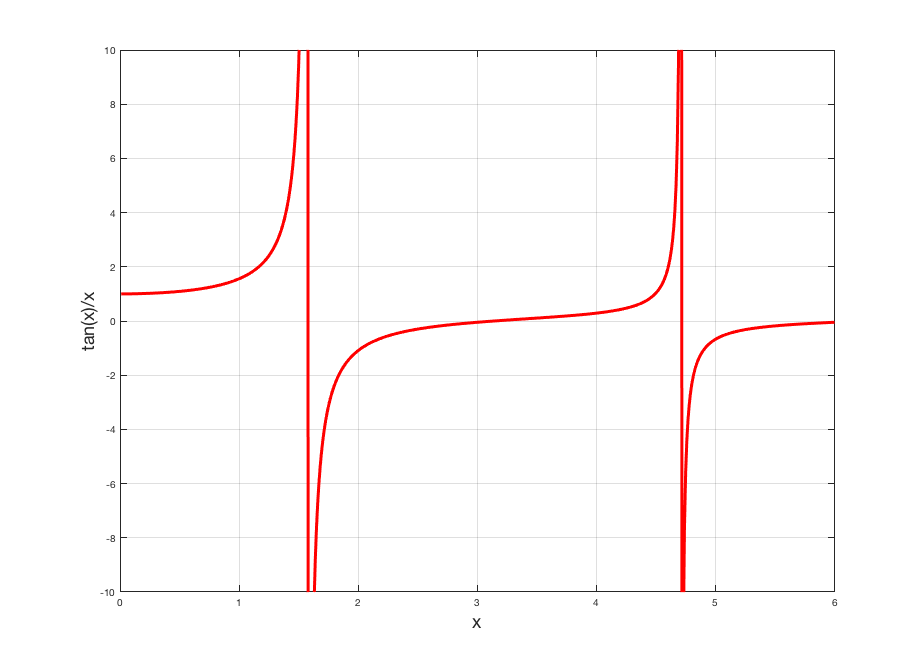
\includegraphics[width=2.2in]{image/tanx_x}
            \caption{势阱散射}
            \label{tanx_x}
            \end{minipage}%
            \begin{minipage}[t]{0.5\linewidth}
            \centering
            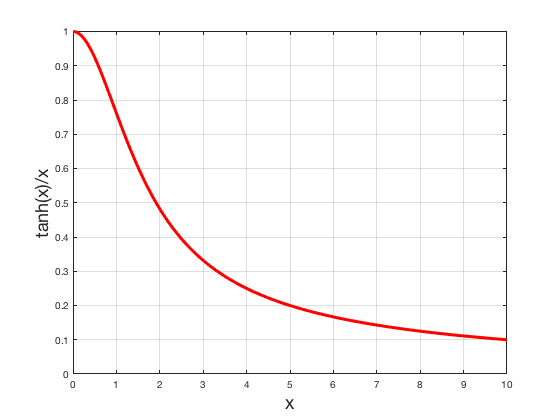
\includegraphics[width=2.2in]{image/tanhx_x}
            \caption{势垒散射}
            \label{tanhx_x}
            \end{minipage}
          \end{figure}

        \subsubsection{Born近似法}
          正如我们在式\eqref{3.2.1:corequestion}中所指出的, 求解散射问题的核心是求解给定能
          量的, 满足散射边界条件的定态薛定谔方程: 
          \begin{equation*}
            \left\{
              \begin{array}{l}
              \left[-\dfrac{\hbar^2}{2m}\nabla^2+V(r)\right]\psi(\vec{r}) = E\psi(\vec{r})\\ \ \\
              \psi(\vec{r}) \overset{r\to\infty}{\longrightarrow}\mathrm{e}^{ikz} + f(\theta)\dfrac{\mathrm{e}^{i\vec{k}\vec{r}}}{r}
              \end{array} \right. 
          \end{equation*}
          
          前面所提到的分波法, 是对无穷远处的波函数关于中心散射势场中的不变量对应的本征波函数做展开, 而Born近似
          则是采用了对薛定谔方程进行变换的思路. 

          注意到$E = \dfrac{k^2\hbar^2}{2m}$, 因此薛定谔方程可以改写为:
          \begin{equation}
            \left(\nabla^2+k^2\right)\psi(\vec{r}) = \dfrac{2m}{\hbar}V(\vec{r})\psi(\vec{r})
          \end{equation}

          上式为一个非齐次赫姆霍兹方程, 采用Green函数法求解此方程. 

          令$G$满足方程:
          \begin{equation}
            \left(\nabla^2+k^2\right)G(\vec{r}-\vec{r'}) = \delta(\vec{r}-\vec{r'})
          \end{equation}

          则, 由格林第二公式, 原方程的解:
          \begin{equation}
            \label{2725:fin}
            \psi(\vec{r}) = \phi(\vec{r}) + \int{}G(\vec{r}-\vec{r'})U(\vec{r'})\psi(\vec{r'})\mathrm{d}\vec{r'}
          \end{equation}

          其中, $U(\vec{r'}) = \dfrac{2m}{\hbar^2}V(\vec{r'})$, $\phi(\vec{r})$是其次方程
          \begin{equation}
            \left(\nabla^2+k^2\right)\phi(r) = 0
          \end{equation}

          的解. 

          因此, 目前求解中心势场散射的全部问题就变为了求解如下两个方程,
          \begin{subequations}
            \begin{align}
              \left(\nabla^2+k^2\right)\phi(r) &= 0\\
              \left(\nabla^2+k^2\right)G(\vec{r}-\vec{r'}) &= \delta(\vec{r}-\vec{r'})
            \end{align}
          \end{subequations}

          首先关注格林函数$G$满足的方程, 对格林函数所满足的方程两侧同时进行Fourier变换:
          \begin{equation}
            \label{fourier_transform_G} 
            \left(\dfrac{1}{2\pi}\right)^3\int(k^2-\eta^2)\mathrm{e}^{i(\vec{r}-\vec{r'})\cdot\vec{\eta}}\tilde{G}(\vec{\eta})%
            \mathrm{d}\vec{\eta} = \left(\dfrac{1}{2\pi}\right)^3\int\mathrm{e}^{i(\vec{r}-\vec{r'})\cdot\vec{\eta}}%
            \mathrm{d}\eta
          \end{equation}

          其中, $\tilde{G}(\vec{\eta})$满足:
          \begin{equation}
            G(\vec{r}-\vec{r'}) = \left(\dfrac{1}{2\pi}\right)^3 \int{}\tilde{G}(\vec{\eta})%
                                        \mathrm{e}^{i(\vec{r}-\vec{r'})\cdot\vec{\eta}}%
                                        \mathrm{d}\vec{\eta} 
          \end{equation}

          从方程\eqref{fourier_transform_G}又可得到, 
          \begin{equation}
            \tilde{G}(\vec{\eta}) = \dfrac{1}{k^2-\eta^2}            
          \end{equation}

          因此, 可解得:
          \begin{equation}
            \begin{aligned}
              G(\vec{r}-\vec{r'}) &= \left(\dfrac{1}{2\pi}\right)^3 \int{}\dfrac{1}{k^2-\eta^2}%
                                          \mathrm{e}^{i(\vec{r}-\vec{r'})\cdot\vec{\eta}}%
                                          \mathrm{d}\vec{\eta}\\
                                  &= \dfrac{1}{8\pi^3}\int_0^{+\infty}\dfrac{1}{k^2-\eta^2}%
                                      \left[\int_0^{2\pi}\mathrm{d}\varphi\int_0^{\pi}\sin\theta%
                                      \mathrm{e}^{i\eta\left|\vec{r}-\vec{r'}\right|}\mathrm{d}\theta\right] %
                                      \eta^2\mathrm{d}\eta\\
                                  &= \dfrac{1}{4\pi^2i\left|\vec{r}-\vec{r'}\right|}\int_{-\infty}^{+\infty}%
                                      \mathrm{d}\eta\;\dfrac{\eta}{k^2-\eta^2} \mathrm{e}^{i\eta\left|\vec{r}-\vec{r'}\right|}\\
                                  &= \dfrac{1}{4\pi^2i\left|\vec{r}-\vec{r'}\right|} \cdot \left(-i\pi\mathrm{e}^%
                                  {ik\left|\vec{r}-\vec{r'}\right|}\right)\\
                                  &= -\dfrac{\mathrm{e}^{ik\left|\vec{r}-\vec{r'}\right|}}%
                                            {4\pi\left|\vec{r}-\vec{r'}\right|}
            \end{aligned}
          \end{equation}

          \begin{figure}
            \centering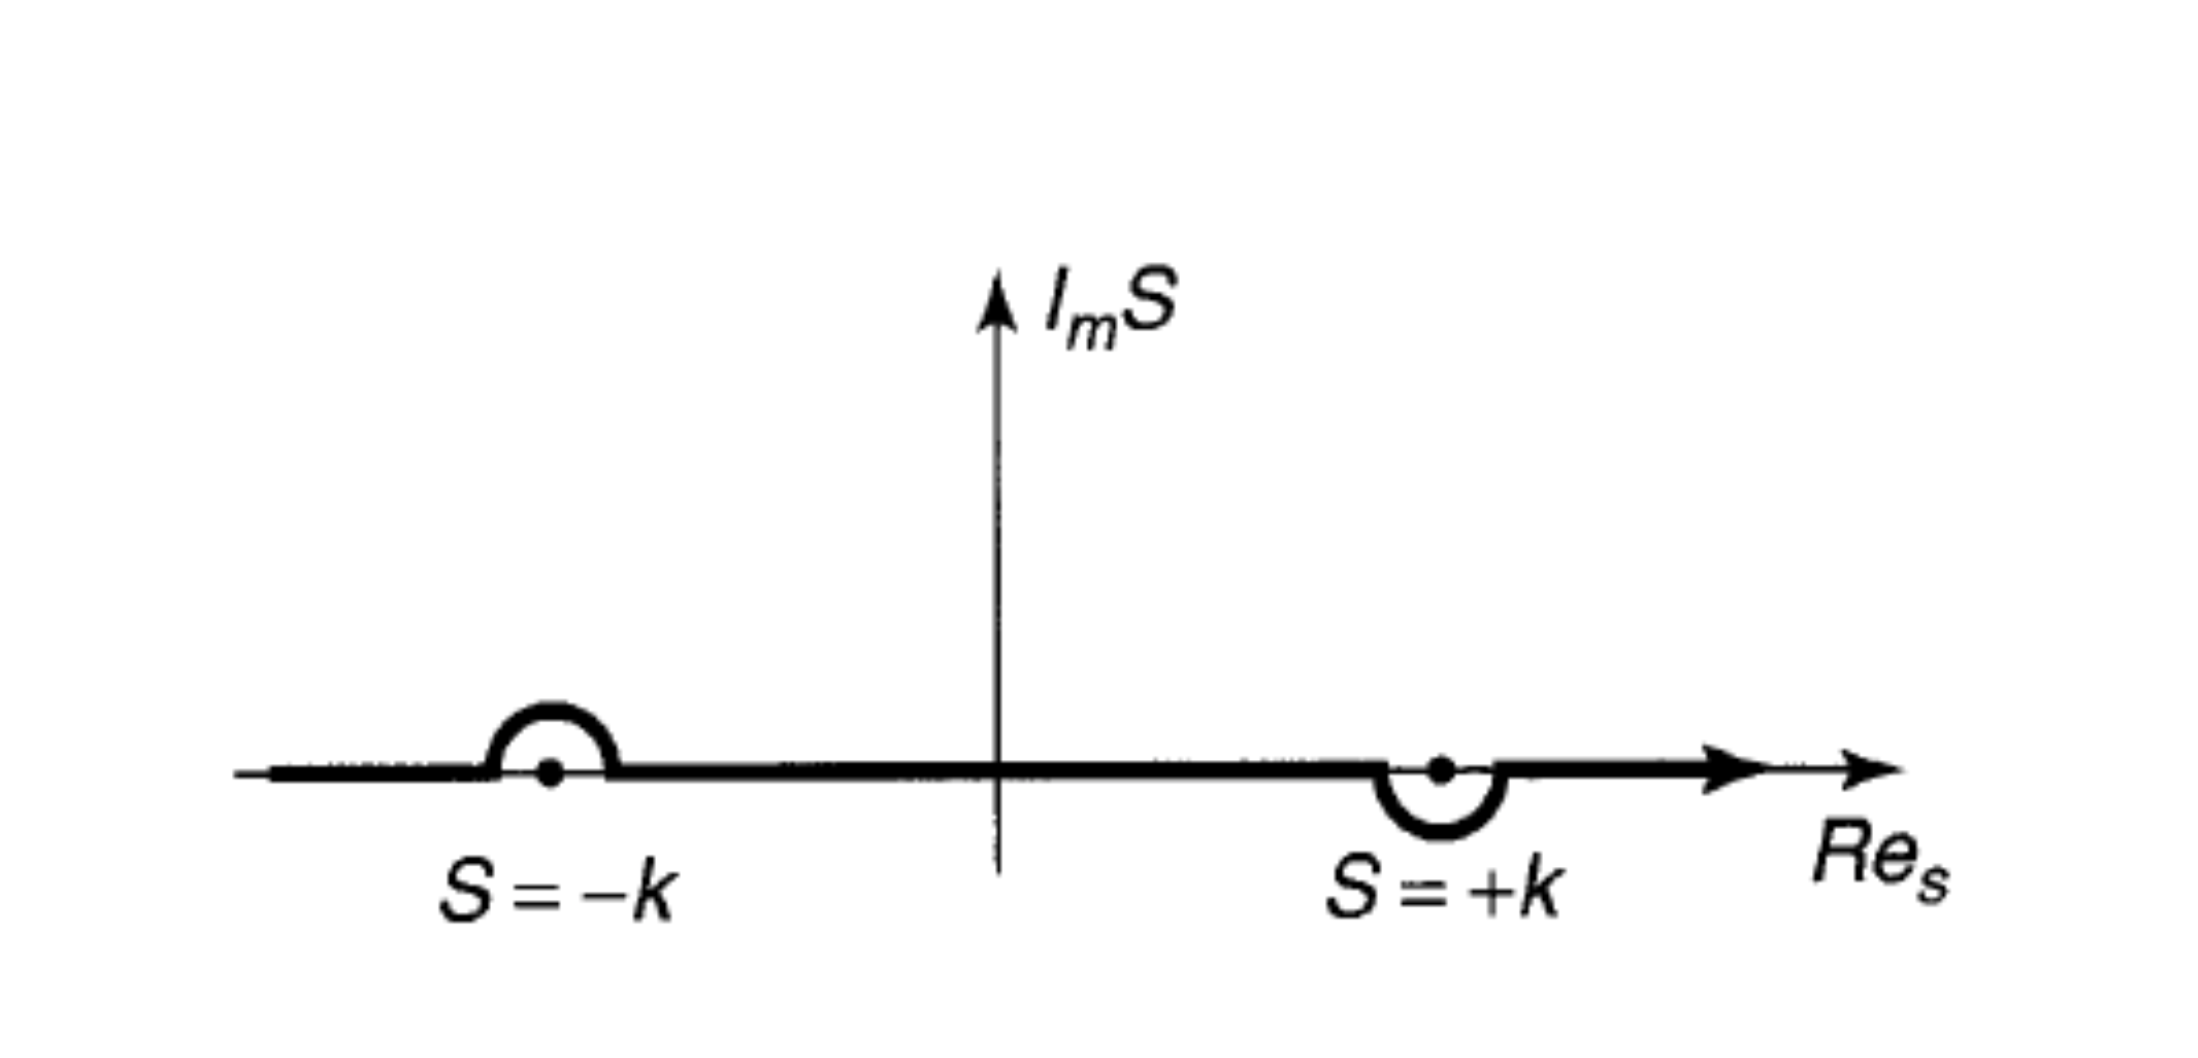
\includegraphics[width=3.5in]{image/Born_route_int}
            \caption{对$\eta$积分绕过奇点的方式}\label{Born_route_int}
          \end{figure} 

          上式中, 对$\eta$的积分值是由留数定理得到的. 选择的积分路径如图\ref{Born_route_int}所示
          \footnote{当然可以选取不同的绕过奇点的积分路径, 但可以证明, 无论如何绕过奇点, 其结果都是等价的.}.

            
          两个留数分别为:
          \begin{equation}
            \begin{aligned}
              \mathrm{Res}(f(k)) &= -\frac{1}{2}\mathrm{e}^{ik\left|\vec{r}-\vec{r'}\right|} \\
              \mathrm{Res}(f(-k)) &= -\frac{1}{2}\mathrm{e}^{-ik\left|\vec{r}-\vec{r'}\right|}
            \end{aligned}
          \end{equation}

          结合上述积分路径, 熟练地运用留数定理后, 对$\eta$的积分结果就是显然的了.

          解决了Green函数, 下面就应该求解$\phi(\vec{r})$所满足的方程了, 由观察可知:
          \begin{equation}
            \phi(\vec{r}) = \mathrm{e}^{ikz}
          \end{equation}
          
          恰好为其一个解.

          这是合理的, 这表明\eqref{2725:fin}等式右端,加号前的部分是入射波, 加号后的部分是反射波. 这是符合无穷远处散射
          波函数的形式的. 
          
          因此, 最终$\psi$满足如下等式:
          \begin{equation}
            \psi(\vec{r}) = \mathrm{e}^{ikz} - \dfrac{m}{2\pi\hbar^2} %
                            \int\dfrac{\mathrm{e}^{ik\left|\vec{r}-\vec{r'}\right|}}%
                                      {\left|\vec{r}-\vec{r'}\right|}V(\vec{r'})%
                                      \psi(\vec{r'})\mathrm{d}\vec{r'}
          \end{equation}

          至此, 所有的求解都是严格的, 我们得到了一个关于$\psi$的积分方程. 这个方程仍然是不容易精确解析求解的. 

          一般的, 求解此方程可在两种层面上进行. 一种是数值求解, 也就是利用所谓的'自洽求解', 不断迭代, 最终得到符合误差范围的数值. 
          另一种是采用微扰近似, 一般常用的是'Born一级近似'.
          
          当入射粒子能量很高, 也就是发生所谓的'高能散射'时, $V(\vec{r})$可视为微扰, 则积分中的$\psi(\vec{r'})$可
          近似等于$\mathrm{e}^{ikz'}$. 于是, 原方程可化为:
          \begin{equation}
            \psi(\vec{r}) \approx \psi_{B1}(\vec{r})= \mathrm{e}^{ikz} - \dfrac{m}{2\pi\hbar^2} %
                                                      \int\dfrac{\mathrm{e}^{ik\left|\vec{r}-\vec{r'}\right|}}%
                                                                {\left|\vec{r}-\vec{r'}\right|}V(\vec{r'})%
                                                                  \mathrm{e}^{ikz'}\mathrm{d}\vec{r'}
          \end{equation}

          对上述近似再进行无穷远处的近似, 
          \begin{equation}
            \lim_{r\to\infty}\left|\vec{r}-\vec{r'}\right| = \lim_{r\to\infty}\sqrt{r^2+r'^2-2\vec{r}\cdot\vec{r'}}%
            \approx r\left(1-\dfrac{\vec{r}\cdot\vec{r'}}{r^2}\right)
          \end{equation}

          将上述近似带入Born一级近似后的波函数:
          \begin{equation}
            \psi_{B1} \approx \mathrm{e}^{ikz} - \dfrac{\mathrm{e}^{i\vec{k}\cdot\vec{r}}}{r}\cdot\dfrac{m}{2\pi\hbar^2} %
                              \int\mathrm{e}^{ik\left(z'-\frac{\vec{r}\cdot\vec{r'}}{r}\right)}V(\vec{r'})%
                                                      \mathrm{d}\vec{r'}
          \end{equation}

          对比之前的无穷远处所设的波函数的形式, 可以知道:
          \begin{equation}
            f(\theta) = -\dfrac{m}{2\pi\hbar^2}\int\mathrm{e}^%
                        {ik\left(z'-\frac{\vec{r}\cdot\vec{r'}}{r}\right)}V(\vec{r'})\mathrm{d}\vec{r'}
          \end{equation}

          \begin{figure}
            \centering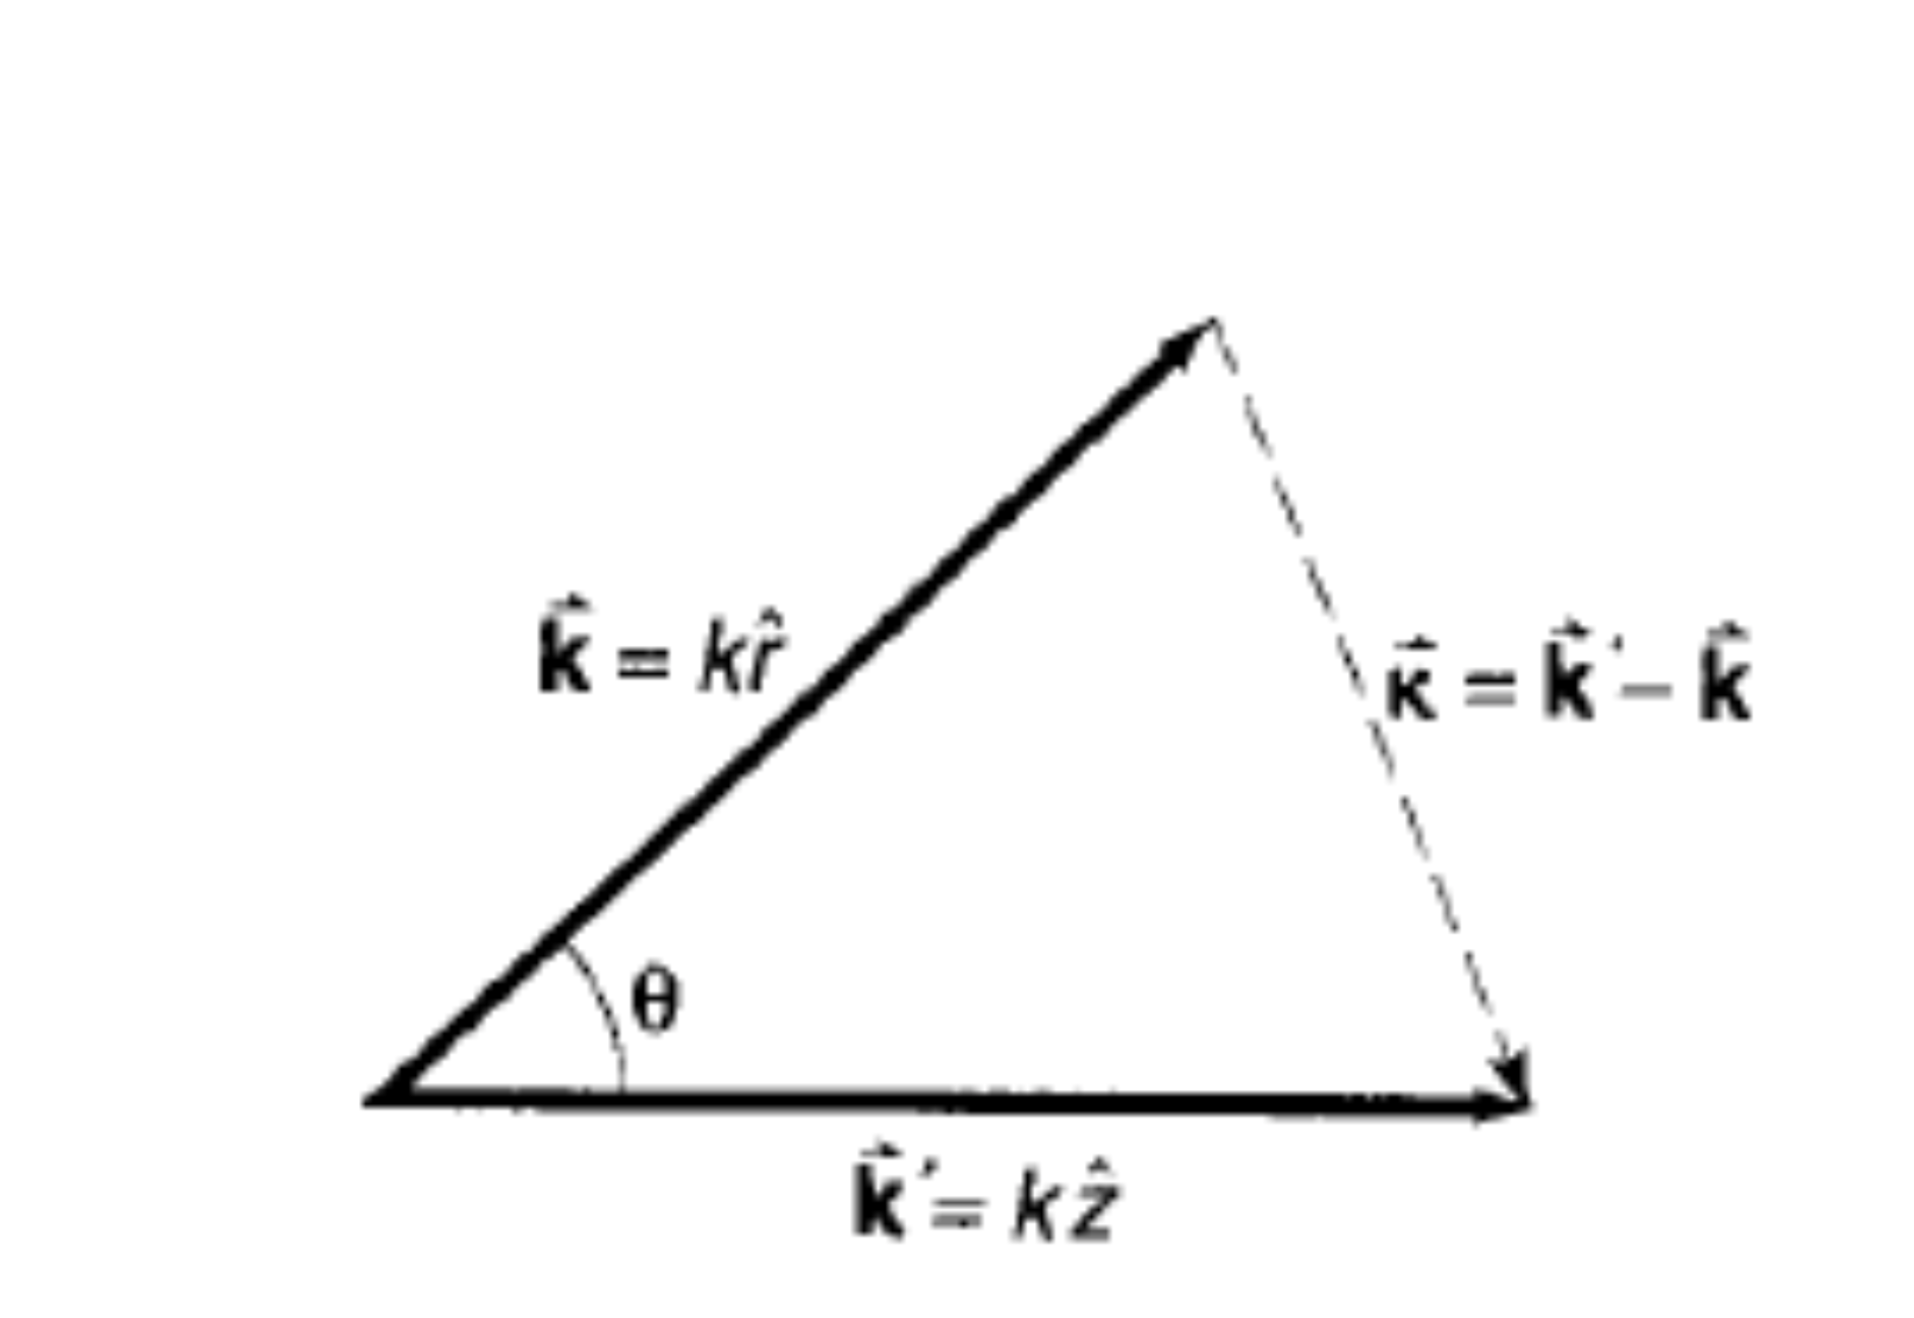
\includegraphics[width=3.5in]{image/direction_kq}
            \caption{向量$\vec{\kappa}$的由来}\label{direction_kq}
          \end{figure} 
          
          结合图\ref{direction_kq}可将$f(\theta)$的形式进一步化简. 
          \begin{equation}
              f(\theta) = -\dfrac{m}{2\pi\hbar^2}\int\mathrm{e}^%
              {i\vec{\kappa}\cdot\vec{r'}}V(\vec{r'})\mathrm{d}\vec{r'} 
          \end{equation}

          更进一步的, 对于球对称势场, 有$V(\vec{r}) = V(r)$, 因此$f(\theta)$可化为更加简洁的形式,
          \begin{equation}
            \label{qdcftdbds}
            f(\theta)= -\dfrac{2m}{\kappa\hbar^2}\int_0^{\infty}rV(r)\sin(\kappa{}r)\mathrm{d}r
          \end{equation}

          因此, 微分散射截面:
          \begin{equation}
            q(\theta) = \dfrac{4m^2}{\kappa^2\hbar^4}\left|\int_0^{\infty}rV(r)\sin(\kappa{}r)\mathrm{d}r\right|^2
          \end{equation}

          其中, 由图\ref{direction_kq}可知:
          \begin{equation}
            \kappa \equiv 2k\sin\frac{\theta}{2}
          \end{equation}

          微分散射截面关于$\theta$的信息体现在$\kappa$里. 

          \textbf{下面探讨Born近似的使用条件}

          回顾Born近似后方程的形式:
          \begin{equation}
            \begin{aligned}
              \psi_{B1}(\vec{r}) &= \mathrm{e}^{ikz} - \dfrac{m}{2\pi\hbar^2} %
                            \int\dfrac{\mathrm{e}^{ik\left|\vec{r}-\vec{r'}\right|}}%
                            {\left|\vec{r}-\vec{r'}\right|}V(\vec{r'})%
                            \mathrm{e}^{ikz'}\mathrm{d}\vec{r'}\\
              &= \mathrm{e}^{ikz} + \psi_s
            \end{aligned}
          \end{equation}

          要使Born近似满足, 则必有:
          \begin{equation}
            \left|\psi_s\right| \ll |\mathrm{e}^{ikz}| \equiv 1
          \end{equation}

          分析$r=0$的情况\footnote{注意, 这里并未用到$r$趋于无穷远处的近似.}
          \begin{equation}
            \begin{aligned}
              \left|\psi_s(0)\right| &= \dfrac{m}{2\pi\hbar^2} \left|\int\dfrac{\mathrm{e}^{ikr'}}{r'}%
                                        V(r')\mathrm{e}^{ikr'\cos\theta}r'^2\sin\theta\mathrm{d}r'%
                                        \mathrm{d}\theta\mathrm{d}\varphi\right|\\
                                      &= \dfrac{m}{\hbar^2} \left|\int\dfrac{\mathrm{e}^{ikr'}}{r'}%
                                      V(r')\dfrac{\mathrm{e}^{ikr'}-\mathrm{e}^{-ikr'}}{ikr'}r'^2\mathrm{d}r'\right|\\
                                      &= \dfrac{m}{k\hbar^2}\left|\int{}V(r')\left(\mathrm{e}^{2ikr'}-1\right)\mathrm{d}r'\right|
            \end{aligned}
          \end{equation}

          使用球方势场具体评估Born近似的使用条件.

          将势场形式:
          \begin{equation}
            V(r) = \left\{
              \begin{array}{ll}
                V_0, & r\leq{}a\\
                0, & r>a
              \end{array}\right. \;\;\;\;\;(V_0>0)
          \end{equation}
          \begin{equation}
            \begin{aligned}
              \left|\psi_s(0)\right| &= \dfrac{m}{k\hbar^2}\left|\int_0^a{}V_0%
                                        \left(\mathrm{e}^{2ikr'}-1\right)\mathrm{d}r'\right|\\
                                      &= \dfrac{mV_0}{2k^2\hbar^2}\left|\mathrm{e}^{2ika}-1-2ika\right|
            \end{aligned}
          \end{equation}

          以下两种情况可满足$|\psi|\ll1$的要求:

          \textbf{1. 入射粒子低能情况下, 若势场很弱, 中心力场力程很短时, Born近似适用}

          在此情况下, 满足$ka\ll1$, 则
          \begin{equation}
            \left|\psi(0)\right| \approx \dfrac{mV_0a^2}{\hbar} \ll 1 
          \end{equation}

          \textbf{2. 入射粒子高能情况下, 即便势场不弱, 中心力场力程很长, 也满足Born近似. 且能量越高, Born近似越精确.}

          在此情况下, 满足
          \begin{equation}
            \left|\psi(0)\right| \approx \dfrac{mV_0a}{k\hbar^2} = \dfrac{\sqrt{m}a}{\sqrt{2}\hbar}%
                                          \dfrac{V_0}{\sqrt{E}} \ll 1 
          \end{equation}

          至此, 我们分析完毕了Born近似的适用条件. 

        \subsubsection{库伦散射}
          了解了两种常用近似后, 我们来尝试着求解另一个看起来十分简单的势场的散射问题: 库伦势场. 

          库伦势场属于长程势, 其形式为:
          \begin{equation}
            V(r) = \dfrac{A}{r}
          \end{equation}

          由分波法条件\eqref{fbftj}, 显然此势场由于是长程势, 分波法对其不适用. 再考虑Born近似:
          
          由于库伦场为球对称势场, 因此将\eqref{qdcftdbds}带入得:
          \begin{equation}
            \begin{aligned}
              f(\theta) &= -\dfrac{2m}{\kappa\hbar^2}\int_0^{\infty}A\sin(\kappa{}r)\mathrm{d}r\\
                        &= \dfrac{2mA}{\kappa\hbar^2}(1-cos(\infty))
            \end{aligned}
          \end{equation}

          $f(\theta)$的值是振荡不收敛的!

          经过以上的分析, 我们陷入了一种十分尴尬的局面. 刚刚花了很大力气得到的两种近似方法, 却连一个简单的库伦势都
          算不出来. 这种无能为力主要原因是库伦力是长程作用力. 为了避免这一效果, 引入所谓的\textbf{'汤川势'}. 
          \begin{equation}
            V(r) = \dfrac{A}{r}\mathrm{e}^{-\alpha{}r}
          \end{equation}

          将上述势能形式带入$f(\theta)$的表达式可得:
          \begin{equation}
            \begin{aligned}
              f(\theta) &= -\dfrac{2m}{\kappa\hbar^2}\int_0^{\infty}rV(r)\sin(\kappa{}r)\mathrm{d}r\\
                        &= -\dfrac{2m}{\kappa\hbar^2}\int_0^{\infty}A\mathrm{e}^{-\alpha{}r}\sin(\kappa{}r)\mathrm{d}r\\
                        &= -\dfrac{2mA}{\kappa\hbar^2}\dfrac{\kappa}{\kappa^2+\alpha^2}
            \end{aligned}
          \end{equation}

          当$\alpha\to0$时, 汤川势退化为库仑势. 此时其$f(\theta)$为:
          \begin{equation}
            \begin{aligned}
              f(\theta) &= -\dfrac{2mA}{\kappa^2\hbar^2}\\
                        &= -\dfrac{mA}{2k^2\hbar^2\sin^2\frac{\theta}{2}}
            \end{aligned}
          \end{equation}

          因此, 其微分散射截面为:
          \begin{equation}
            q(\theta) = \dfrac{m^2A^2}{4\hbar^4k^4\sin^4\frac{\theta}{2}}
          \end{equation}

          该结果与精确求解结果完全一致.\footnote{库伦散射的精确求解见, 曾谨言 量子力学 卷I(13.5), 卷II(10.2)}

          库伦势散射特点可总结为: A.散射主要集中在小角度附近; B.散射截面与入射粒子的能量的平方成反比.
              
        \subsubsection{全同粒子碰撞}
          全同粒子组成的多粒子系统的态矢对粒子对换的操作具有对称或反对称性, 分别对应于波色子和费米子. 根据角动量
          理论, 对于两个全同粒子体系的自旋耦合态有如下关系\footnote{何来???}:
          \begin{equation}
            |s_1, s_2, S,M\rangle = (-1)^{2s_1-S}|s_2, s_1, S,M\rangle
          \end{equation}

            对于全同粒子, 满足关系: 
            \begin{equation}
              s_1 = s_2
            \end{equation}

            因此可列出下表:
          
          \begin{table}[H]
          \caption{全同粒子的波函数对称关系}
            \begin{tabular}{ccc|ccc}
              \toprule
              \multicolumn{3}{c|}{Boson, $s_1=s_2$为整数}&\multicolumn{3}{c}{Fermion, $s_1=s_2$为半整数}\\
              \multicolumn{3}{c|}{$|s_1, s_2, S,M\rangle = (-1)^{S}|s_2, s_1, S,M\rangle$} &%
              \multicolumn{3}{c}{$|s_1, s_2, S,M\rangle = -(-1)^{S}|s_2, s_1, S,M\rangle$}\\
              \hline
              总波函数=&自旋波函数$\otimes$&空间波函数&总波函数=&自旋波函数$\otimes$&空间波函数\\
              \hline
              对称&S=奇数(反对称)&反对称&反对称&S=奇数(对称)&反对称\\
              \hline
              对称&S=偶数(对称)&对称&反对称&S=偶数(反对称)&对称\\
              \bottomrule
            \end{tabular} 
          \end{table} 

          由上表可见, 无论是波色子还是费米子, 当S=奇数时, 体系空间波函数一定是反对称的; 当S=偶数时, 体系的
          空间波函数一定是对称的!

          在前文中, 由于靶粒子质量远远大于入射粒子, 我们实际上是把质心系近似成了靶粒子不动的参考系. 在讨论全同粒子的
          对撞时, 此假设不再成立, 需要考虑质心系下的情况. 在质心系中, 两个全同粒子的碰撞是对撞. 对于全同粒子对撞, 
          需要考虑空间波函数是对称的或是反对称的. 

          \textbf{1. 描述具有空间对称性的入射波:}
          \begin{equation}
            \psi_i = \mathrm{e}^{ikz} + \mathrm{e}^{-ikz}
          \end{equation}

          式中, $z = z_1-z_2$, 为相对坐标.
          
          由此, 散射边界条件可写作:
          \begin{equation}
            \psi_i = \mathrm{e}^{ikz} + \mathrm{e}^{-ikz} + \left[f(\theta)+f(\pi-\theta)\right]%
                      \dfrac{\mathrm{e}^{ikr}}{r}
          \end{equation}

          微分散射截面为:
          \begin{equation}
            q(\theta) = |f(\theta)+f(\pi-\theta)|^2
          \end{equation}

          \textbf{2. 描述具有空间反对称性的入射波:}
          \begin{equation}
            \psi_i = \mathrm{e}^{ikz} - \mathrm{e}^{-ikz}
          \end{equation}

          式中, $z = z_1-z_2$, 仍然为相对坐标.
          
          由此, 散射边界条件可写作:
          \begin{equation}
            \psi_i = \mathrm{e}^{ikz} - \mathrm{e}^{-ikz} + \left[f(\theta)-f(\pi-\theta)\right]%
                      \dfrac{\mathrm{e}^{ikr}}{r}
          \end{equation}

          微分散射截面为:
          \begin{equation}
            q(\theta) = |f(\theta)-f(\pi-\theta)|^2
          \end{equation}

          由上面的分析可见, 空间波函数的对称性影响微分散射截面!

          \begin{figure}
            \begin{minipage}[t]{0.5\linewidth}
            \centering
            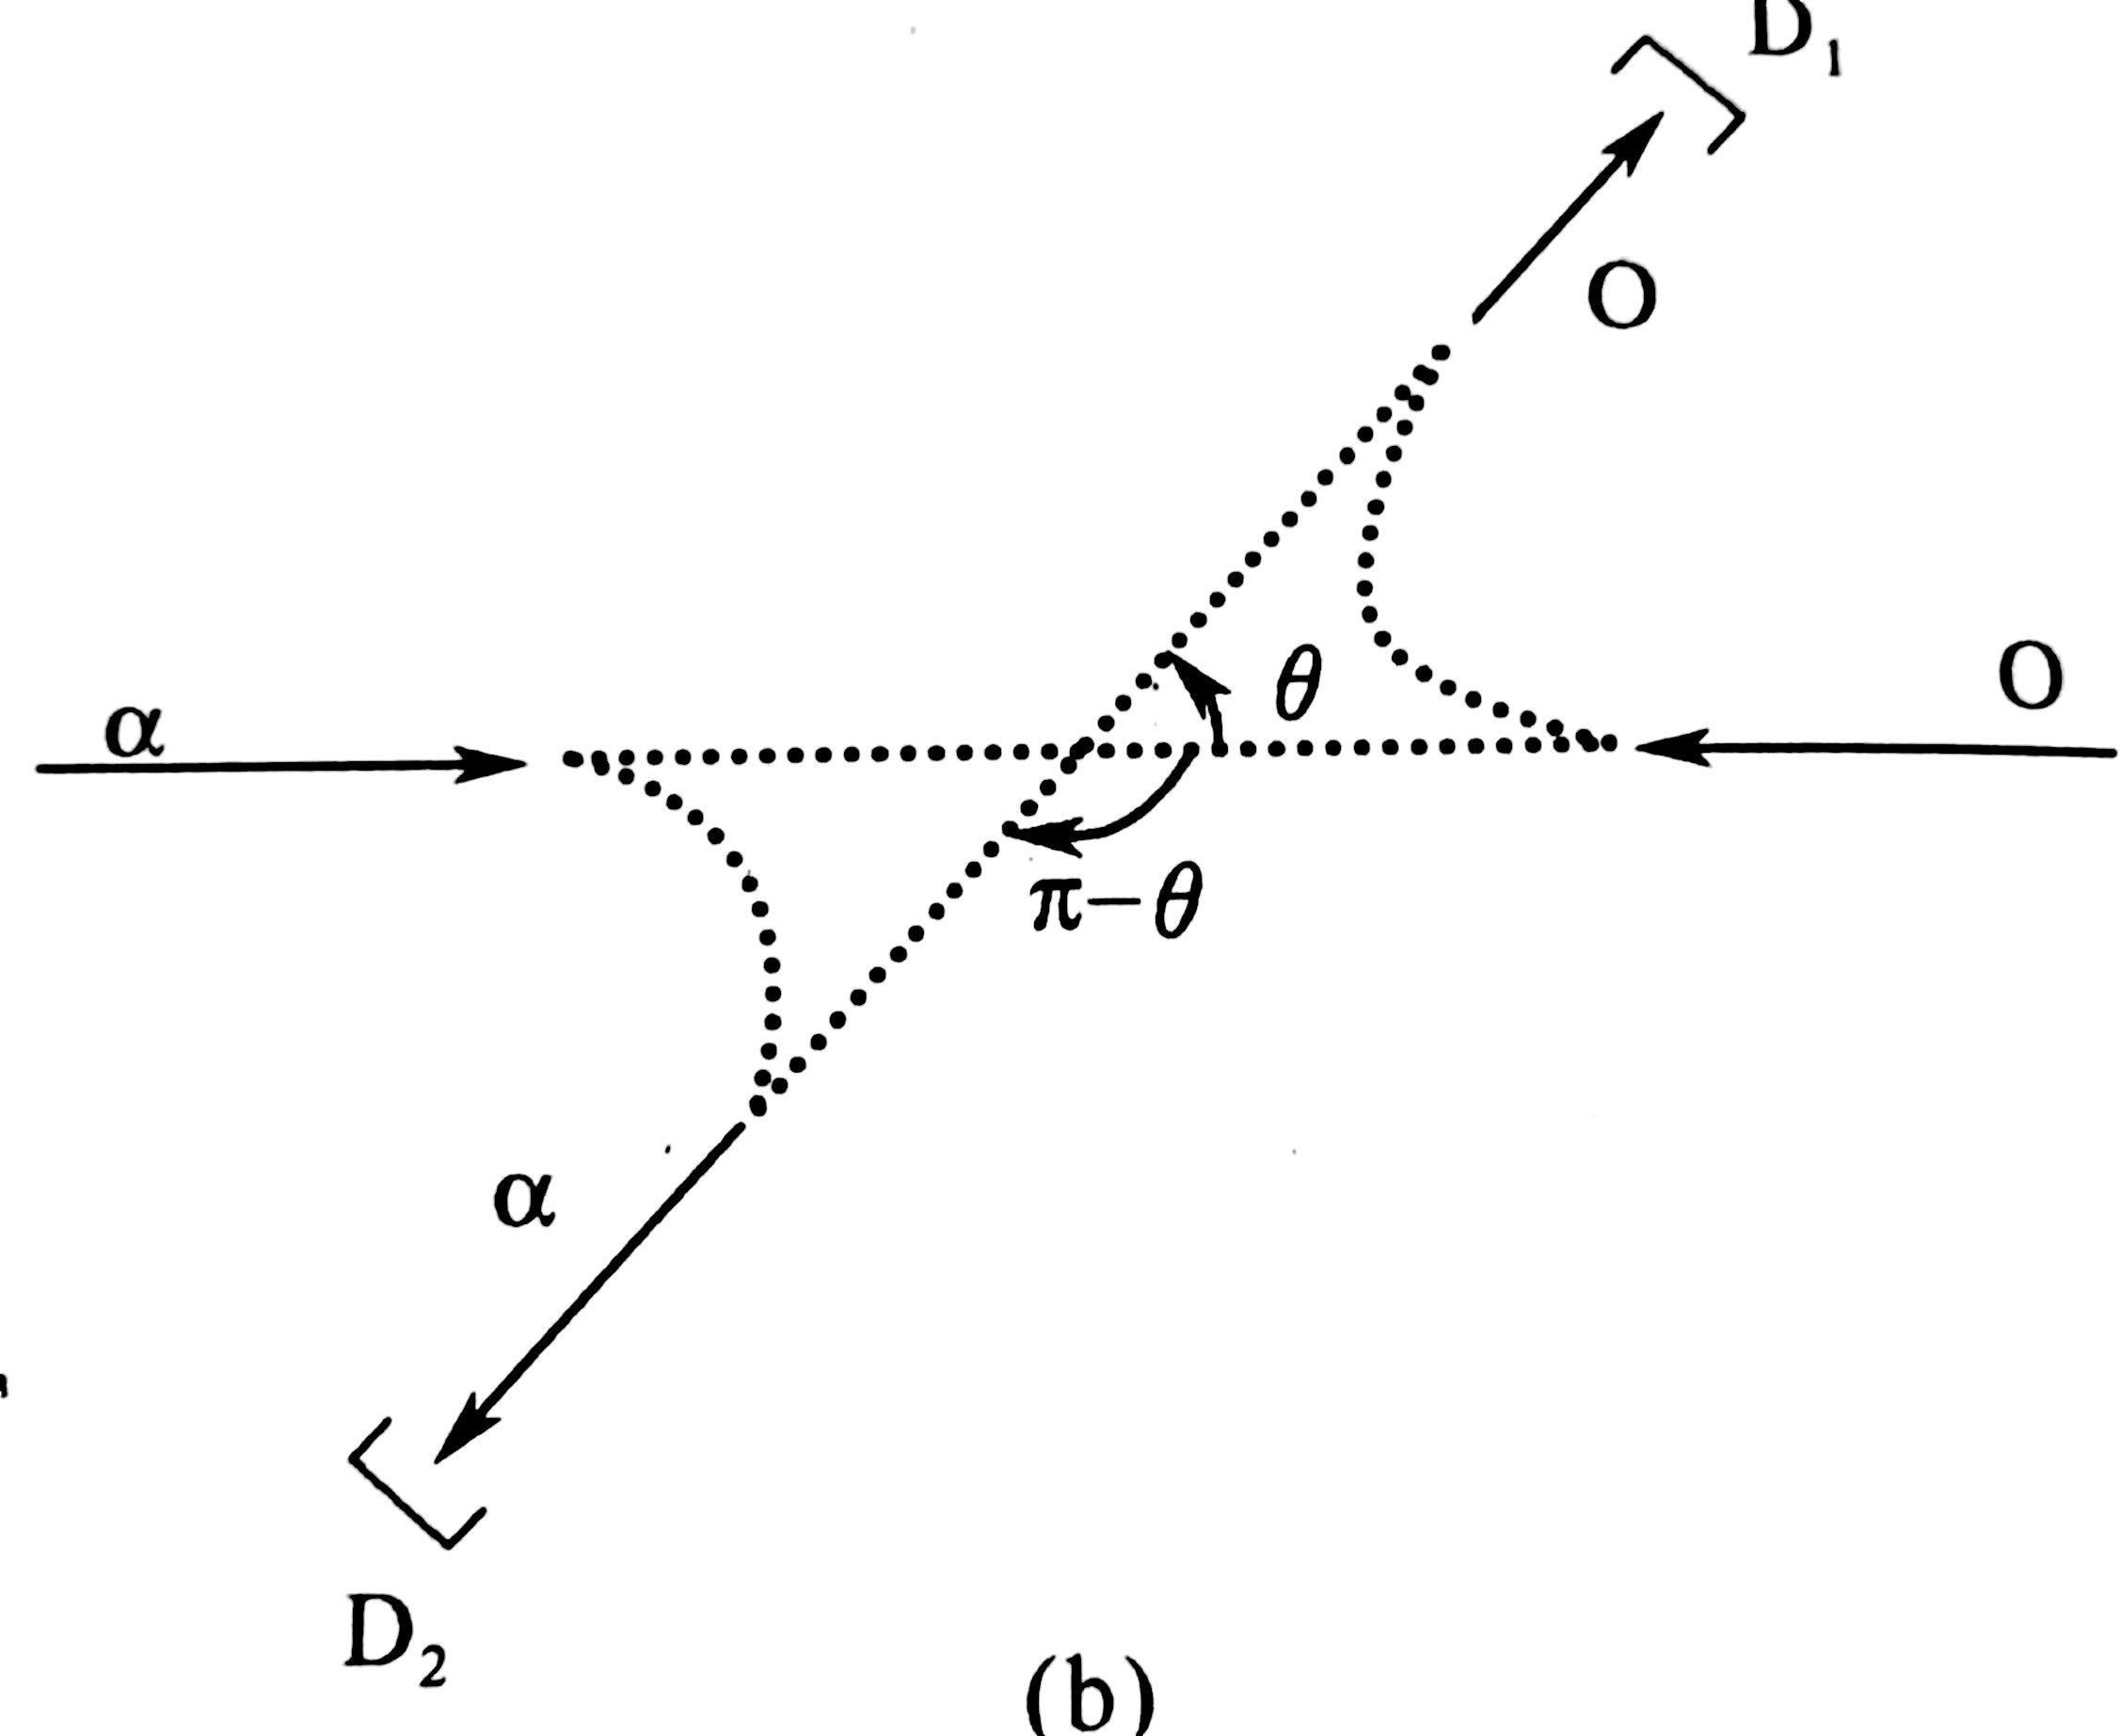
\includegraphics[width=2.2in]{image/scattering_1}
            \caption{第一种散射方式}
            \label{scattering_1}
            \end{minipage}%
            \begin{minipage}[t]{0.5\linewidth}
            \centering
            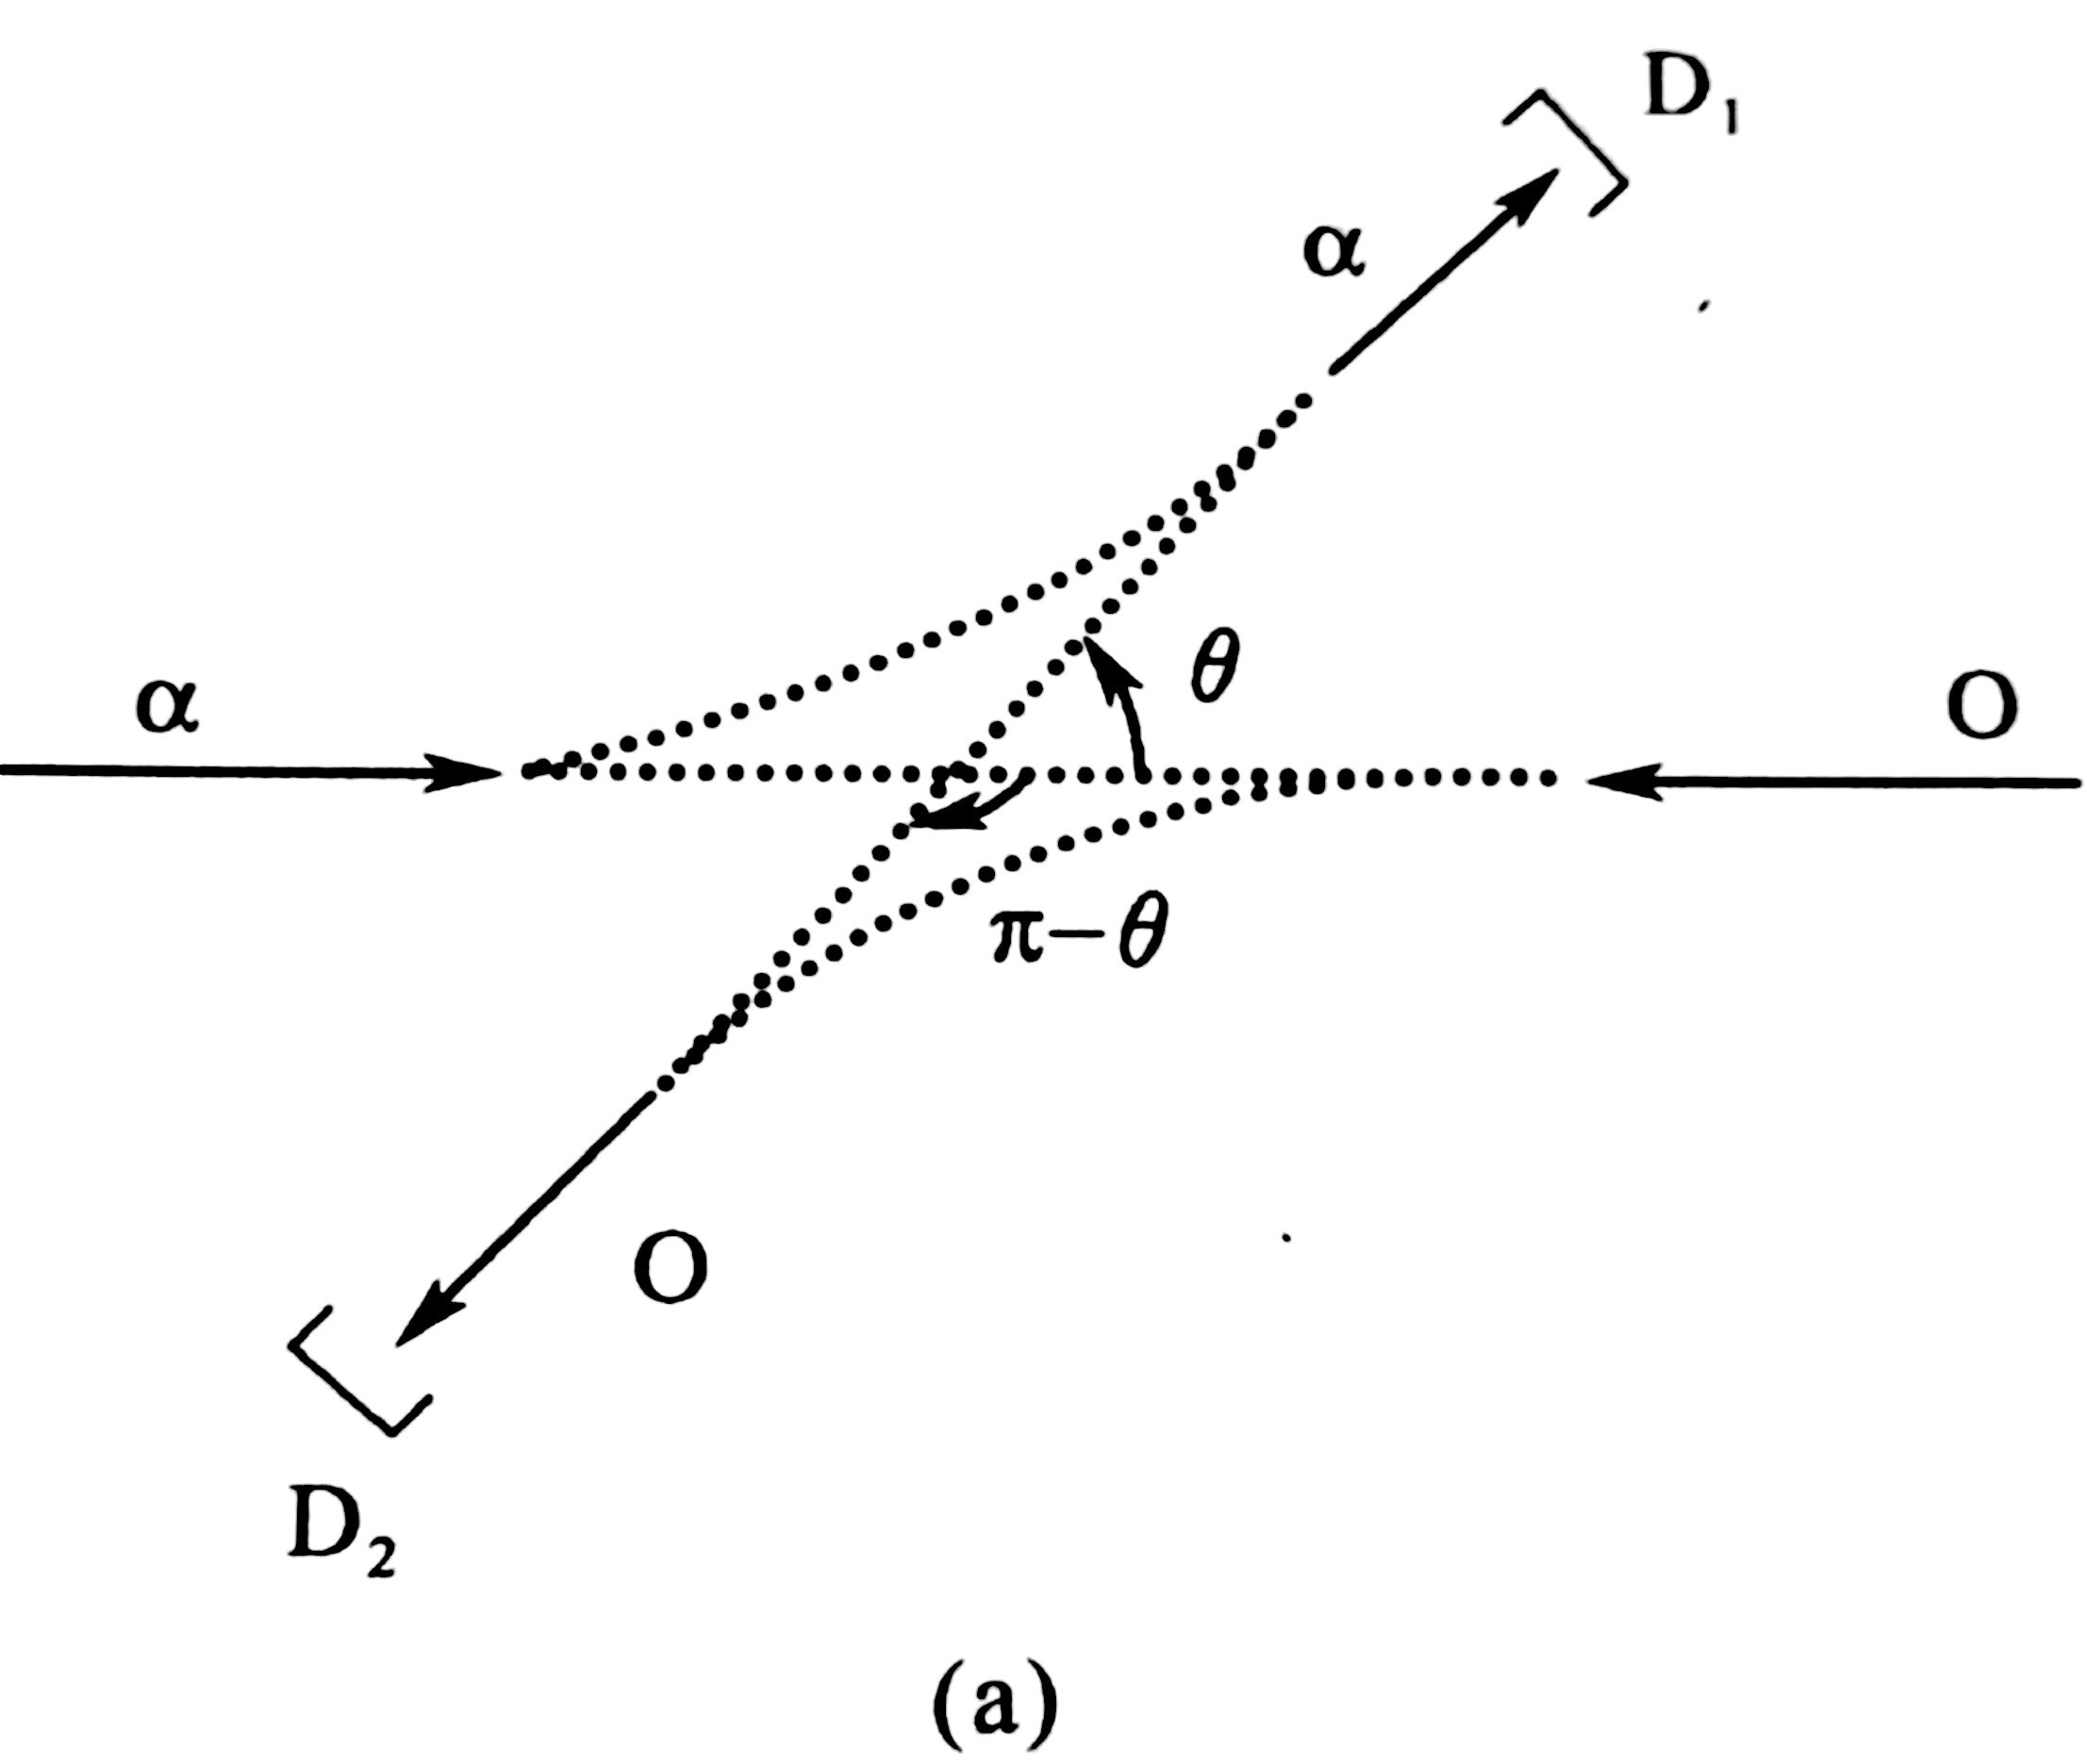
\includegraphics[width=2.2in]{image/scattering_2}
            \caption{第二种散射方式}
            \label{scattering_2}
            \end{minipage}
          \end{figure}

          \textbf{下面讨论全同粒子的微分散射截面的问题.} 
          首先思考非全同粒子的散射问题.  
          参与散射的是一个$\alpha$粒子与一个$^{16}O$粒子.则图\ref{scattering_1}与图\ref{scattering_2}
          所示的两种情况是可以区分的, 且整个体系的散射截面由两个粒子的散射截面独立的提供. 也就是说:
          \begin{equation}
            q(\theta) = |f(\theta)|^2 + |f(\pi-\theta)|^2
          \end{equation}
            
          然而, 如果发生散射的是全同粒子. 例如两个入射粒子都是$\alpha$粒子. 则图\ref{scattering_1}与图\ref{scattering_2}
          所示的两种情况是不可区分的. 而且体系的散射截面有两个粒子产生的干涉的贡献.\footnote{许多人喜欢这样的描述:
          由于粒子不可区分, 因此他们之间存在干涉. 个人认为这样的描述是会让人产生误解的, 不可区分性和干涉效应应该都是
          全同粒子体系不同方面的属性, 他们之间没有明显的因果关系.}

          也即:
          \begin{equation}
            \begin{aligned}
              q(\theta) &= |f(\theta) + f(\pi-\theta)|^2 \\
                        &= |f(\theta)|^2 + |f(\pi-\theta)|^2 + 2f^*(\theta)f(\pi-\theta) + f(\theta)f^*(\pi-\theta)\\
                        &= |f(\theta)|^2 + |f(\pi-\theta)|^2 + 2\mathrm{Re}[f^*(\theta)f(\pi-\theta)]
            \end{aligned}
          \end{equation}

          干涉相的存在,使得全同粒子散射与非全同粒子散射有不同的特点, 比如

          \emph{1. 在$\theta=\frac{\pi}{2}$处, 全同粒子散射的微分散射截面的值是非全同粒子的2倍.}

          \emph{2. 全同粒子的散射截面, 在质心系中, 总是关于$\theta = \frac{\pi}{2}$对称.}

          \textbf{为了进一步理解全同粒子的对撞问题, 下面举一个实际的例子. 自旋为$\dfrac{1}{2}$的全同粒子的对撞(电子).}

          应该知道, 自旋为$\dfrac{1}{2}$的两个电子组成的系统角动量空间中存在四个态, 一个自旋三重态, 一个自旋单态. 自旋
          单态的总自旋为0, 自旋三重态的总自旋为1. 由前面的分析知道, 总自旋为偶数时, 空间波函数对称; 总自旋为奇数时, 空间
          波函数反对称. 于是:
          \begin{equation}
            \left\{
            \begin{aligned}
              q_s(\theta) = |f(\theta)+f(\pi-\theta)|^2, \;\;\;\;\;\; &  S=0,\\
              q_A(\theta) = |f(\theta)-f(\pi-\theta)|^2, \;\;\;\;\;\; &  S=1.
            \end{aligned}\right.
          \end{equation}

          对于一个均匀的系统, 其出射的电子对组成的总自旋系统是均匀分布在各个态上的. 因此, 总的微分散射截面是:
          \begin{equation}
            \begin{aligned}
              q(\theta) &= \dfrac{1}{4}q_s(\theta)+ \dfrac{3}{4}q_A(\theta)\\
                        &= \dfrac{1}{4}|f(\theta)+f(\pi-\theta)|^2 + \dfrac{3}{4}|f(\theta)-f(\pi-\theta)|^2\\
                        &= |f(\theta)|^2 + |f(\pi-\theta)|^2 - \dfrac{1}{2}[f^*(\theta)f(\pi-\theta) + f(\theta)f^*(\pi-\theta)]\\
                        &= |f(\theta)|^2 + |f(\pi-\theta)|^2 - \mathrm{Re}[f^*(\theta)f(\pi-\theta)]
            \end{aligned}
          \end{equation}

          从另一个角度看双电子散射, 也即不把两个电子耦合为一个态, 也可以得到相同的结果, 具体的操作如表\ref{2ele_table}所示. 
          表中实验设备由图\ref{scattering_1}与图\ref{scattering_2}给出. 

          \begin{table}
            \centering
            \begin{spacing}{1.4}
            \caption{极化电子的碰撞自旋取向与微分散射截面}
            \label{2ele_table}
            \begin{tabular}{ccccc}
              \toprule
              入射电子(1)  &  靶电子(2) & $D_1$测得电子 & $D_2$测的电子 & 微分散射截面\\
              \hline
              $\uparrow$ & $\uparrow$ & $\uparrow$ & $\uparrow$ & $|f(\theta)-f(\pi-\theta)|^2$\\
              \hline
              $\downarrow$ & $\downarrow$ & $\downarrow$ & $\downarrow$ & $|f(\theta)-f(\pi-\theta)|^2$\\
              \hline
              $\uparrow$ & $\downarrow$ & $\begin{array}{l}\uparrow\\ \downarrow\end{array}$%
              &$\begin{array}{l}\downarrow\\\uparrow\end{array}$%
              &$\begin{array}{l}|f(\theta)|^2 \\|f(\pi-\theta)|^2 \end{array}$\\
              \hline
              $\downarrow$ & $\uparrow$ & $\begin{array}{l}\uparrow \\ \downarrow\end{array}$%
              &$\begin{array}{l}\downarrow\\\uparrow\end{array}$% 
              &$\begin{array}{l}|f(\pi-\theta)|^2 \\|f(\theta)|^2 \end{array}$\\ 
              \bottomrule 
            \end{tabular} 
            \end{spacing}
          \end{table}

          粒子体系处在表\ref{2ele_table}中的四个态的概率各是$\frac{1}{4}$, 因此最终, 体系整体的微分
          散射截面为: 
          \begin{equation*}
            q(\theta) = |f(\theta)|^2 + |f(\pi-\theta)|^2 - \mathrm{Re}[f^*(\theta)f(\pi-\theta)]
          \end{equation*}

          这与之前所得的结果是完全一样. 

          下面利用分波法具体计算一个非全同粒子散射的例子, 作为本节的结束.

          \emph{低能e-p(电子质子)散射, 只考虑S波. 设e-p相互作用表示为}
          \begin{equation}
            V = V_0 + V_{\sigma}(r)\hat{s}_e\cdot\hat{s}_p
          \end{equation}

          \emph{设入射粒子和靶粒子处于极化状态, 入射中子自旋向前(正z轴), 质子(靶)自旋向后, 即}
          \begin{equation}
            \Psi_i = \left(\begin{array}{c}1\\0\end{array}\right)_e%
                     \left(\begin{array}{c}0\\1\end{array}\right)_p%
                      \mathrm{e}^{ikz}
          \end{equation}

          \emph{设$f_1, f_3$分别代表自旋单重态和自旋三重态的S波散射振幅, 计算e-p散射的散射截面.}

          注意到在上述哈密顿量描述的体系中, 总角动量平方以及总角动量的$z$分量为守恒量. 因此, 将上述入射态向
          $\{\hat{S}^2, \hat{S_z}\}$的共本态上展开. 
          \begin{equation}
            \Psi_i = \dfrac{1}{\sqrt{2}}\left(\chi_{00}+\chi_{10}\right)\mathrm{e}^{ikz}
          \end{equation}

          由于总角动量为守恒量, S=0和S=1两部分分波各自独立进行散射, 即:
          \begin{equation}
            \begin{aligned}
              \chi_{00}\mathrm{e}^{ikz} \longrightarrow f_1\chi_{00}\;\dfrac{\mathrm{e}^{ikz}}{r}\\
              \chi_{10}\mathrm{e}^{ikz} \longrightarrow f_3\chi_{10}\;\dfrac{\mathrm{e}^{ikz}}{r}
            \end{aligned}
          \end{equation}

          进而, 整体的散射波函数为:
          \begin{equation}
            \lim_{r\to\infty}\Psi_{SC} = \dfrac{1}{\sqrt{2}}\left(f_1\chi_{00}+f_3\chi_{10}\right)%
                                                            \dfrac{\mathrm{e}^{ikz}}{r}
          \end{equation}

          微分散射截面为:
          \begin{equation}
            \begin{aligned}
              q(\theta) &= \left|\dfrac{1}{\sqrt{2}}\left(f_1\chi_{00}+f_3\chi_{10}\right)\right|^2\\
                        &= \dfrac{1}{2}\left(|f_1|^2+|f_3|^2\right)
            \end{aligned}
          \end{equation}

          总散射截面为:
          \begin{equation}
            Q = \int\mathrm{d}\Omega\;q(\theta) = 2\pi\left(|f_1|^2+|f_3|^2\right)
          \end{equation}

          至此, 我们求解出了e-p散射的散射截面. 

    \section{WKB近似}
      \subsection{定态近似方法的回顾}

      表\ref{weiraohuigu}总结了微扰近似方法的求解核心问题和适用范围.

      \begin{table}[H]
        \centering
        \caption{近似方法的回顾}
        \begin{spacing}{1.4}
        \label{weiraohuigu}
        \begin{tabular}{c|c|cccc}
          \toprule
          求解体系特征  &  求解参量 & \multicolumn{4}{c}{近似/求解方法}\\
          \hline
          束缚态 & $\left(E_n, \varphi_n\right)$&微扰论 & 变分法 & WKB近似 &\\
          \hline
          散射态 & $\left(T, R, q(\theta)\right)$ & 传递矩阵 & 分波法 & Born近似 & WKB近似\\
          \bottomrule 
        \end{tabular} 
        \end{spacing}
      \end{table}

        \subsubsection{定态微扰论}

          \textbf{对于两个量子体系:$\hat{H}_0$与$\hat{H} = \hat{H}_0 + \hat{W}= \hat{H}_0 + \lambda\hat{H}'$. 
          若$\hat{W}$相对于$\hat{H}_0$可视为微扰, 也即$\lambda$是一个小量, 则$\hat{H}_0$与$\hat{H}$的本征值和本征矢是相似的. 
          可将其能量和波函数分别按表示微扰程度的小量幂次展开, 带入定态方程逐级求解.} 

          \begin{figure}[H]
            \centering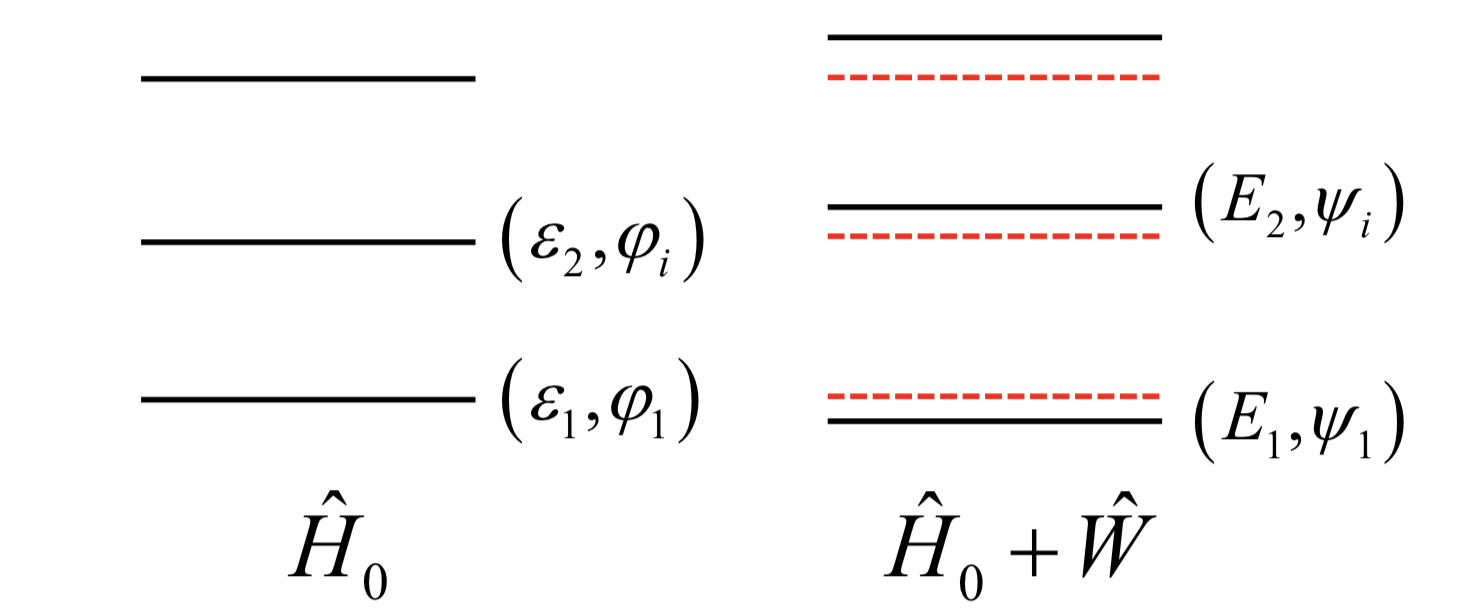
\includegraphics[width=3.5in]{image/perturbation_theory}
            \caption{定态微扰论}
          \end{figure}

          也就是:
          \begin{equation}
            \begin{aligned}
              \hat{H}_0&\varphi_n = \varepsilon_n\varphi_n \\
              E_n &= E_n^{(0)} + E_n^{(1)} +E_n^{(2)} + \ldots\\
                  &= \varepsilon_n + \lambda\varepsilon_n'^{(1)} + \lambda^2\varepsilon_n'^{(2)}+\ldots\\
              \psi_n &= \psi_n^{(0)} + \psi_n^{(1)} +\psi_n^{(2)} + \ldots\\
                  &= \varphi_n + \lambda\varphi_n'^{(1)} + \lambda^2\varphi_n'^{(2)}+\ldots\\
            \end{aligned}
          \end{equation}

          \textbf{1. 非简并微扰理论}

          如果仅考虑能量的前两级近似, 那么能量与波函数的形式分别可以写作:
          \begin{equation}
            \begin{aligned}
              E_k &\approx \varepsilon_k + E_k^{(1)} + E_k^{(2)}\\
              \psi_k &\approx \varphi_k + \psi_k^{(1)}
            \end{aligned}
          \end{equation}

          其中,
          \begin{equation}
            \begin{aligned}
              W_{ij} &= \langle\varphi_i\left|\hat{W}\right|\varphi_j\rangle\\
              E_k^{(1)} &= W_{kk}\\
              E_k^{(2)} &= \sum_{n\ne{}k}\dfrac{W_{nk}W_{kn}}{\varepsilon_k-\varepsilon_n}\\
              \psi_k^{(1)} &= \sum_{n\ne{}k}\dfrac{W_{nk}}{\varepsilon_k-\varepsilon_n}\varphi_n
            \end{aligned}
          \end{equation}

          \textbf{2. 简并微扰理论}

          仅考虑能量的第一级近似, 又意识在微扰中到对简并能级劈裂的大部分贡献都来源于$H_0$中能量简并子空间所对应的微扰
          子空间上.\footnote{这句话可能是难以理解的, 具体的可以参考下面的推导} 于是, 求解简并微扰问题就化为了求解如
          下定态Schr\"odinger方程的问题, 
          \begin{equation}
            \begin{aligned}
              \hat{H}_k\psi_{km} &= E_{km}\psi_{km} \\
              H_k &=(\hat{H}_0)_k + \hat{W}_k\\
                  &=\begin{bmatrix}
                    \varepsilon_k & 0 & \ldots & 0\\
                    0 & \varepsilon_k & \ldots & 0\\
                    \vdots & \vdots & \ddots & \vdots\\
                    0 & 0 & \ldots & \varepsilon_k\\
                    \end{bmatrix} + %
                    \begin{bmatrix}
                      W_{11} & W_{12} & \ldots & W_{1M}\\
                      W_{21} & W_{22} & \ldots & W_{2M}\\
                      \vdots & \vdots & \ddots & \vdots\\
                      W_{M1} & W_{M2} & \ldots & W_{MM}\\
                      \end{bmatrix}  
            \end{aligned}
          \end{equation}

          求解出上述矩阵的本征值和本征矢后, 我们就可以声称已经完成了简并微扰近似了. 上述矩阵可以看成是从一大块装饰着各种水果蛋糕上%
          切下的表面只有白色奶油的一小块. 
          
          \textbf{3. 近简并微扰理论}

          近简并微扰的套路与简并微扰的套路是完全一样的, 只不过此时$(\hat{H}_0)_k$的对角元不再是单值的了.
          \begin{equation}
            \begin{aligned}
              \hat{H}_k\psi_{km} &= E_{km}\psi_{km} \\
              H_k &=(\hat{H}_0)_k + \hat{W}_k\\
                  &=\begin{bmatrix}
                    \varepsilon_k+\delta\varepsilon_1 & 0 & \ldots & 0\\
                    0 & \varepsilon_k+\delta\varepsilon_2 & \ldots & 0\\
                    \vdots & \vdots & \ddots & \vdots\\
                    0 & 0 & \ldots & \varepsilon_k+\delta\varepsilon_M\\
                    \end{bmatrix} + %
                    \begin{bmatrix}
                      W_{11} & W_{12} & \ldots & W_{1M}\\
                      W_{21} & W_{22} & \ldots & W_{2M}\\
                      \vdots & \vdots & \ddots & \vdots\\
                      W_{M1} & W_{M2} & \ldots & W_{MM}\\
                      \end{bmatrix}  
            \end{aligned}
          \end{equation}

          求解出上述矩阵的本征值和本征矢之后, 近简并微扰近似就完成了. 

          下面举一个微扰理论应用的实际例子. 
          
          \emph{类氢原子的正常Zeeman效应.}

          磁场引起的附加项为:
          \begin{equation}
            \hat{H}_z = \dfrac{e}{2mc}B\left(\hat{L}_z+2\hat{S}_z\right)
          \end{equation}

          若将上述附加能视为微扰, 并应用定态微扰论采用能量本征态$|nlm_lm_s\rangle$对微扰项进行处理, 可得到
          加入磁场附加能微扰后体系的能量:
          \begin{equation}
            E_{nlm_lm_s} = -\dfrac{13.6eV}{n^2} + \mu_BB_{ext}(m_l+2m_s)
          \end{equation}

          我们非常幸运的恰好选取了一个$\hat{W}$和$\hat{H}_0$的共本态. 这样一来, 微扰项在此基底下恰好是对角化的, 
          因此上述结果已经算是严格解了. 但这仍然不妨碍我们使用这个例子作为微扰求解问题套路演示的一个简单的范例. 
        
        \subsubsection{变分法}
          变分法做近似的基本思想是: 随机选取一个波函数$\psi$, 只要$\psi$不是体系的基态波函数, 则必有:
          \begin{equation}
            \langle\psi|\hat{H}|\psi\rangle \geq \langle\psi_0|\hat{H}|\psi_0\rangle = E_0  
          \end{equation}

          因此, 需要找到这样一个波函数, 使得上式右端的值达到最小值. 就可以声称找了基态波函数. 

          同样的, 当自认为找到最低能量值对应的基态波函数后, 可以取与之正交的函数集, 在此集合中继续寻找第一激发态的波函数:
          \begin{equation}
            \langle\psi|\hat{H}|\psi\rangle \geq \langle\psi_1|\hat{H}|\psi_1\rangle = E_1  
          \end{equation}

      \subsection{WKB近似解及连接公式}

        \textbf{WKB近似是一种准经典的近似方法. }在1926年由 Wentzel, Kramers及Brillouin提出.
        它是解决一维定态薛定谔方程近似解的一种技术, 对计算束缚态能级和势垒穿透率都是非常有用的, 也适用于中心力场的径向方程.
        \textbf{WKB近似方法就其本身而言, 有两个基本问题: 其一是,在远离转折点处的波函数近似解;其二是, 在转折点处的连接条件.}

        \subsubsection{WKB近似解}
          薛定谔方程:
          \begin{equation}
            \psi''(x) = -\dfrac{2m}{\hbar^2}\left[E-V(x)\right]\psi(x)
          \end{equation}

          对于简单的阶梯势场, 在经典允许区其解为:
          \begin{equation}
            \psi(x) = A\mathrm{e}^{\pm{}ikx} = A\mathrm{e}^{\pm\frac{ipx}{\hbar}}
          \end{equation}

          而在经典禁区, 其解为:
          \begin{equation}
            \begin{aligned}
              \psi(x) &= A\mathrm{e}^{\pm\alpha{}x}\\
              \alpha &= \sqrt{\dfrac{2m(V_0-E)}{\hbar^2}}
            \end{aligned}
          \end{equation}

          对于一般的势场$V(x)$经典允许区内的解的形式可写作:
          \begin{equation}
            \psi(x) = A'\mathrm{e}^{\frac{iS(x)}{\hbar}}
          \end{equation}

          将上述特解带入schr\"odinger方程, 
          \begin{equation}
            \label{3510:Sx}
            i\hbar{}S''(x)-\left[S'(x)\right]^2 = -2m\left[E-V(x)\right]
          \end{equation}

          接下来就要使用WKB近似最为关键的一步:将$S(x)$按$\hbar$ \footnote{$\hbar = 1.05\times10^{-34}J\cdot{}S$}展开.
          \begin{equation}
            S(x) = S_0(x) + \hbar{}S_1(x) + \hbar^2{}S_2(x) + \ldots
          \end{equation}

          这是完全让人匪夷所思的操作. 

          将上述展开式带入\eqref{3510:Sx}中, 可得:
          \begin{equation}
            i\hbar\left[S_0''(x)+\hbar{}S_1''(x)+\ldots\right]-\left[S_0'(x)+\hbar{}S_1'(x)+\ldots\right]^2 = -2m\left[E-V(x)\right]
          \end{equation}

          将上述方程左右两边整理成$\hbar$次方项系数对应相等的形式, 并只取一级近似, 则有:
          \begin{equation}
            \begin{aligned}
              \left[S_0'(x)\right]^2 = 2m\left[E-V(x)\right]\\
              iS_0''(x) - 2S_0'(x)S_1'(x) = 0
            \end{aligned}
          \end{equation}

          解上述方程可得:
          \begin{equation}
            \begin{aligned}
              S_0(x) &= \pm\int^xp(x')\mathrm{d}x'\\
              S_1'(x) &= \dfrac{i}{2}\dfrac{S_0''(x)}{S_0'(x)} \\   
                      &= \dfrac{i}{2}[\ln{}p(x)]'\\
              S_1(x) &=  \dfrac{i}{2}\ln{}p(x)   
            \end{aligned}
          \end{equation}

          其中,  $p(x)=\sqrt{2m(E-V(x))}$

          因此, 在经典允许区内, 波函数的一级近似为:
          \begin{equation}
            \begin{aligned}
            \psi(x) &\approx A'\mathrm{e}^{\frac{i(S_0+\hbar{}S_1)}{\hbar}} \\
                    &=\dfrac{A'}{\sqrt{p(x)}}\mathrm{e}^{\pm\frac{i}{\hbar}\int^xp(x')\mathrm{d}x'}\\
                    &=\dfrac{A}{\sqrt{k(x)}}\mathrm{e}^{\pm{}i\int^xk(x')\mathrm{d}x'}
            \end{aligned}  
          \end{equation}
          
          显然 ,$k(x) = \dfrac{1}{\hbar}\sqrt{2m(E-V(x))}$.
          在经典禁区内, 求解过程是完全类似的, 只需将上述结果中的$k(x)$换为$i\alpha(x)$即可. 其中, 
          $\alpha(x) = \dfrac{1}{\hbar}\sqrt{2m(V(x)-E)}$
          \begin{equation}
            \psi(x) \approx%
            \dfrac{B}{\sqrt{\alpha(x)}}\mathrm{e}^{\pm\int^x\alpha(x')\mathrm{d}x'}
          \end{equation}

          有两点需要说明: 一是, 上式实际上包含了两个解; 二是, 上述公式中e指数上的积分没有规定积分下限, 实际上这个下限是
          任意的. 因为不同的积分下限只会使最终结果相差一个相位因子, 只需保证同一个体系中积分下限选取相同, 从而不产生
          相对相位差即可. 也可以理解为, 该相位因子可以被系数A或B吸收. 

        \subsubsection{WKB一级近似解成立的条件}

          由上面的推导, 可知, 要使此一级近似成立, 需要满足以下条件:
          \begin{equation}
            \Bigg\Downarrow
            \begin{aligned}
              \left|\dfrac{\hbar{}S_1}{S_0}\right| &\ll 1\\
              \left|\dfrac{\hbar[\ln(p(x))]'}{2p(x)}\right| &\ll 1\\
              \left|\dfrac{\hbar{}p(x)'}{2p^2(x)}\right| &\ll 1\\
              \left|\dfrac{\hbar\frac{\mathrm{d}V(x)}{\mathrm{d}x}}{4m(E-V(x))\sqrt{2m(E-V(x))}}\right| &\ll 1\\
            \end{aligned}
          \end{equation}

          由上述条件可知: \textbf{如果$V(x)$随$x$的变化很缓慢, 并且粒子的``动能''[E-V(x)]又很大, WKB一级近似成立. 
          显然, 在$E=V(x)$附近WKB近似无效!}

          下面讨论一个具体的例子:

          \emph{无限深垂直势阱底部崎岖不平, 其势函数为:}
          \begin{equation}
            V(x) = \left\{\begin{array}{ll}
              f(x), & 0<x<a\\
              \infty, & elsewhere
            \end{array}\right. 
          \end{equation}

          \emph{并且体系的能量满足:}
          \begin{equation}
            E_{min} > f_{min}(x)
          \end{equation}

          \emph{求解此体系的本征能级}

          在这个例子中, 前面分析的WKB近似条件显然是满足的, 因为该体系不存在$E=V(x)$的部分. 

          设体系的WKB波函数为, 
          \begin{equation}
            \begin{aligned}
              \psi(x) &= \dfrac{1}{\sqrt{k(x)}} %
              \left\{A_1\mathrm{e}^{-i\int_0^xk(x')\mathrm{d}x'} + %
                    A_2\mathrm{e}^{i\int_0^xk(x')\mathrm{d}x'}\right\}\\
                    &= \dfrac{A}{\sqrt{k(x)}}\sin\left[\int_0^xk(x')\mathrm{d}x'+\delta\right]
            \end{aligned}
          \end{equation}

          由边界条件可推出如下结论:
          \begin{equation}
            \label{WKB:wxssj}
            \begin{aligned}
              \left\{\begin{array}{lcl}
                \psi(0) = 0 & \Longrightarrow & \delta = 0\\
                \psi(a) = 0 & \Longrightarrow & \int_0^ak(x)\mathrm{d}x = n\pi
              \end{array}\right.
            \end{aligned}
          \end{equation}

          最终, 得到能量的满足的条件为:
          \begin{equation}
            \int_0^{a} \sqrt{2m(E-V(x))}\mathrm{d}x = n\pi\hbar
          \end{equation}

          带入一个特殊情况验证: 如果$V(x) = 0$, 则体系就完全退化为一维无限深势阱问题:
          \begin{equation}
            \int_0^{a} \sqrt{2mE}\mathrm{d}x = n\pi\hbar \Longrightarrow E_n = \dfrac{n^2\pi^2\hbar^2}{2ma^2}
          \end{equation}
       
        \subsubsection{WKB近似的连接公式}

          观察图\ref{WKB_potencial}所示的一般势场的形式, 由前面所得到的WKB近似解, 该势场可分为5个区域: 
          远离a点的经典I区, 在a点附近的临界区II区, 中间经典允许区III区, b点附近的临界区IV区, 远离b点的经典禁区V区.

          \begin{figure}
            \centering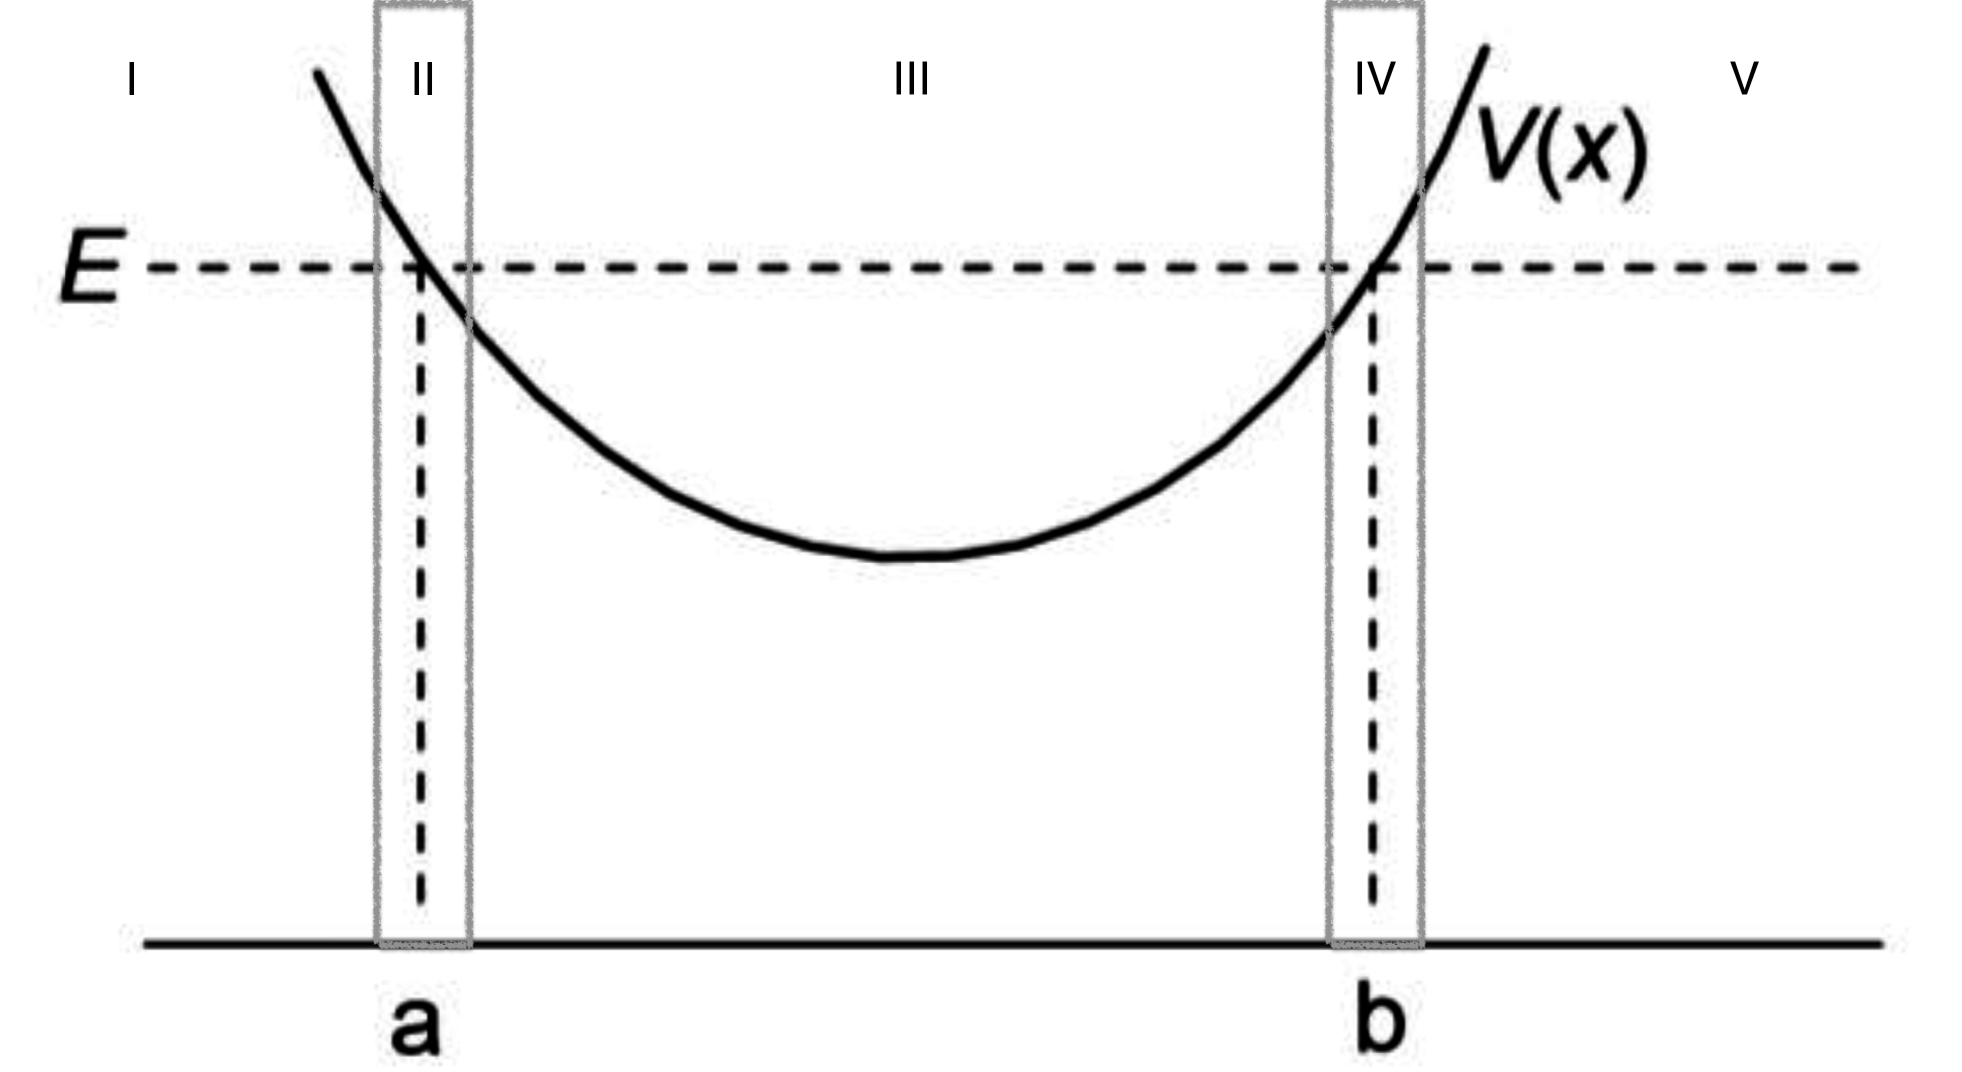
\includegraphics[width=3.5in]{image/WKB_potencial}
            \caption{WKB近似中一般势场的分区}
            \label{WKB_potencial}
          \end{figure}

          考虑在此势场下, 波函数在无穷远处为0, 再结合之前的推导得到该体系波函数的形式为:
          \begin{equation}
            \psi(x) = \left\{\begin{array}{ll}
              \dfrac{B}{\sqrt{\alpha(x)}}\mathrm{e}^{-\int_x^a\alpha(x')\mathrm{d}x'}, & x<a-\Delta\\
              \mathrm{(!!UNKNOWN!!)} & a-\Delta<x<a+\Delta\\
              \dfrac{1}{\sqrt{k(x)}}\left\{A_1\mathrm{e}^{-i\int_a^xk(x')\mathrm{d}x'} + %
                A_2\mathrm{e}^{i\int_a^xk(x')\mathrm{d}x'}\right\}, &  a+\Delta<x<b-\Delta\\
              \mathrm{(!!UNKNOWN!!)} & b-\Delta<x<b+\Delta\\
              \dfrac{C}{\sqrt{\alpha(x)}}\mathrm{e}^{-\int_b^x\alpha(x')\mathrm{d}x'}, & x>b+\Delta              
            \end{array}\right.
          \end{equation}

          在上述临界区域II, IV中, WKB近似显然是不满足的, 因此该区域中波函数的形式仍是未知的. 
          于是需要在这个区域中建立特殊的波函数形式, 也就是需要得到一个合理的 
          连接I,III,V区的连接公式. 
          
          建立此连接公式的基本思想是: 在转折点附近建立一个修补区, 求解该区域内的薛定谔方程,
          得到修补区的形式解, 在修补区的两端边界与WKB解相连接, 从而找到WKB波函数的连接公式. 
          
          \textbf{以b点所在的IV区为例.} 

          设IV区中势场近似有如下形式:
          \begin{equation}
            V'(x) = V(b)+\left.\dfrac{\partial{}V(x)}{\partial{}x}\right|_{x=b}(x-b) 
          \end{equation}

          这其实就是对势场进行了线性近似处理. 
          同时, 注意到$V(b)\approx{}E$, 因此, 有:
          \begin{equation}
            V'(x) = E + g\cdot(x-b)
          \end{equation}

          将其带入定态Schr\"odinger方程可得:
          \begin{equation}
            \psi_p''(x) - \dfrac{2mg}{\hbar^2}(x-b)\psi_p(x) = 0
          \end{equation}

          通过换元, 令$\xi = \left(\dfrac{2mg}{\hbar^2}\right)^{\frac{1}{3}}(x-b)$, 可将上述方程化简后解析求解: 
          \begin{equation}
            \psi_p''(\xi) = \xi\psi_p(\xi) \Longrightarrow \psi_p = C_1A_i(\xi) + C_2B_i(\xi)
          \end{equation}

          上式的方程被称为Airy方程, 其解中的$A_i, B_i$分别为$\frac{1}{3}$阶Bessel函数. 

          注意到, 由于$\xi$的分母中含有$\hbar^2$, 因此当x稍微远离b的时候就可以将$\xi$视为一个接近无穷的值.

          首先观察IV与V区的边界处, 此时$\xi\to+\infty$:

          结合$\frac{1}{3}$阶Bessel函数在\textbf{正无穷远处}的近似形式, 就可得到从IV区趋近于(IV, V)区边界时的波函数的形式,
          \begin{equation}
            \label{WKB:b:2}
            (\psi_p)_{\mathrm{IV}\to{}\mathrm{V}} = C_1\dfrac{1}{2\sqrt{\pi}\xi^{\frac{1}{4}}}\mathrm{e}^{-\frac{2}{3}\xi^{\frac{3}{2}}}+%
                     C_2\dfrac{1}{2\sqrt{\pi}\xi^{\frac{1}{4}}}\mathrm{e}^{\frac{2}{3}\xi^{\frac{3}{2}}}
          \end{equation}

          结合之前V区WKB近似的结果, 由V区趋近该边界的波函数形式应为:
          \begin{equation}
            \label{WKB:b:1}
            \begin{aligned}
              (\psi_{\mathrm{WKB}})_{\mathrm{V}\to{}\mathrm{IV}} &= \dfrac{C}{\sqrt{\alpha(x)}}\mathrm{e}^{-\int_b^x\alpha(x')\mathrm{d}x'}\\
                                        &= \dfrac{C}{\left(\dfrac{2mg}{\hbar^2}\right)^{\frac{1}{6}}\xi^{\frac{1}{4}}}\mathrm{e}^{-\frac{2}{3}\xi^{\frac{3}{2}}}
            \end{aligned}
          \end{equation} 

          要将两区连接起来, 需要使\eqref{WKB:b:2}和\eqref{WKB:b:1}两式形式相同. 因此, 可以得到:
          \begin{equation}
            \label{WKB:connect:1}
            \left\{\begin{array}{l}
              C_1 = \dfrac{2\sqrt{\pi}}{\left(\dfrac{2mg}{\hbar^2}\right)^{\frac{1}{6}}}C\\
              C_2 = 0
            \end{array}\right.
          \end{equation}

          再研究IV与III的连接处:此时$\xi\to-\infty$:
          
          结合$\frac{1}{3}$阶Bessel函数在\textbf{负无穷远处}的近似形式, 以及上面分析的系数$C_2=0$的条件 
          ,就可得到从IV区趋近于(IV, III)区边界时的波函数的形式,
          \begin{equation}
            \label{WKB:b:3}
            (\psi_p)_{\mathrm{IV}\to\mathrm{III}} = \dfrac{C_1}{\sqrt{\pi}(-\xi)^{\frac{1}{4}}}%
            \sin\left[\dfrac{2}{3}(-\xi)^{\frac{3}{2}}+\dfrac{\pi}{4}\right]
          \end{equation}

          结合之前III区WKB近似的结果, 由III区趋近该边界的波函数形式应为:
          \begin{equation}
            \label{WKB:b:4}
            \begin{aligned}
              (\psi_{\mathrm{WKB}})_{\mathrm{III}\to\mathrm{IV}} &= \dfrac{1}{\sqrt{k(x)}} %
              \left\{A_1\mathrm{e}^{i\int_x^bk(x')\mathrm{d}x'} + %
                    A_2\mathrm{e}^{-i\int_x^bk(x')\mathrm{d}x'}\right\}\\
                    &= \dfrac{A}{\sqrt{k(x)}}\sin\left[\int_x^bk(x')\mathrm{d}x'+\delta\right]\\
                    &= \dfrac{A}{\left(\dfrac{2mg}{\hbar^2}\right)^{\frac{1}{6}}(-\xi)^{\frac{1}{4}}}%
                    \sin\left[\int_x^bk(x')\mathrm{d}x'+\delta\right]\\
                    &= \dfrac{A}{\left(\dfrac{2mg}{\hbar^2}\right)^{\frac{1}{6}}(-\xi)^{\frac{1}{4}}}%
                    \sin\left[\dfrac{2}{3}(-\xi)^{\frac{3}{2}}+\delta\right]
            \end{aligned}
          \end{equation}

          要将两区连接起来, 需要使\eqref{WKB:b:3}和\eqref{WKB:b:4}两式形式相同. 因此, 可以得到:
          \begin{equation}
            \label{WKB:connect:2}
            \left\{\begin{array}{l}
              C_1 = \dfrac{\sqrt{\pi}}{\left(\dfrac{2mg}{\hbar^2}\right)^{\frac{1}{6}}}A\\
              \delta = \dfrac{\pi}{4}
            \end{array}\right.
          \end{equation}

          综合\eqref{WKB:connect:1}和\eqref{WKB:connect:2}两式, 就可以得到:
          \begin{equation}
            \left\{
            \begin{aligned}
              A &= 2C\\
              \delta &= \dfrac{\pi}{4}
            \end{aligned}\right.
          \end{equation}

          至此, 我们解出了b点附近临界区IV中的波函数. 

          \textbf{对$a$点附近的求解也是类似的}

          将$a, b$的求解结果整理如下:
          \begin{equation}
            \psi_a(x) = \left\{\begin{array}{ll}
              \dfrac{B}{\sqrt{\alpha(x)}}\mathrm{e}^{-\int_x^a\alpha(x')\mathrm{d}x'}, & x<a-\Delta\\
              \\
              \dfrac{2\sqrt{\pi}B}{\left(\dfrac{2mg'}{\hbar^2}\right)^{\frac{1}{6}}}A_i(-\xi') & a-\Delta<x<a+\Delta\\
              \\
              \dfrac{2B}{\sqrt{k(x)}}\sin\left[\int_a^xk(x')\mathrm{d}x'+\dfrac{\pi}{4}\right], &  x>a+\Delta            
            \end{array}\right.
          \end{equation}
          \begin{equation}
            \psi_b(x) = \left\{\begin{array}{ll}
              \dfrac{2C}{\sqrt{k(x)}}\sin\left[\int_x^bk(x')\mathrm{d}x'+\dfrac{\pi}{4}\right], & x<b-\Delta\\
              \\
              \dfrac{2\sqrt{\pi}C}{\left(\dfrac{2mg}{\hbar^2}\right)^{\frac{1}{6}}}A_i(\xi) & a-\Delta<x<a+\Delta\\ 
              \\
              \dfrac{C}{\sqrt{\alpha(x)}}\mathrm{e}^{-\int_b^x\alpha(x')\mathrm{d}x'}, & x>b+\Delta              
            \end{array}\right.
          \end{equation}
   
          要将$\psi_a$与$\psi_b$在III区形式统一起来, 则必有\footnote{两个角度相等只在某些特殊的
          $x$处成立, 因此不能作为统一III区函数形式时的条件, 但两角度相加为$n\pi$可以是对所有$x$都成立的.}:
          \begin{equation}
            \left\{
            \begin{aligned}
              &B = C\\
              &\left[\int_x^bk(x')\mathrm{d}x'+\dfrac{\pi}{4}\right]+%
               \left[\int_a^xk(x')\mathrm{d}x'+\dfrac{\pi}{4}\right]= n\pi
            \end{aligned}\right.\;\;\;(n=1,2,3,\ldots)
          \end{equation}

          也即:
          \begin{equation}
            \label{WKB:wuchuizhibi}
            \left\{
            \begin{aligned}
              &B = C\\
              &\int_a^bk(x)\mathrm{d}x= \left(n+\dfrac{1}{2}\right)\pi
            \end{aligned}\right. \;\;\;\;\;\;\;(n=0,1,2,\ldots)
          \end{equation}

          将上述第二个等式进一步变换, 做成环路积分的形式, 并注意在由$b\to{}a$的积分过程中, 粒子的动量应该变为
          由$a\to{}b$中动量的相反数:
          \begin{equation}
            \begin{aligned}
              \oint_{ab}p(x)\mathrm{d}x &= \int_a^b\hbar{}k(x)\mathrm{d}x + \int_b^a-\hbar{}k(x)\mathrm{d}x \\
                                        &= 2\left(n+\dfrac{1}{2}\right)\pi\hbar \\
                                        &= \left(n+\dfrac{1}{2}\right)h\\
            \end{aligned}
          \end{equation}

          这正是``波尔-索末菲量子化条件''\footnote{您可能更熟悉这样形式的``波尔-索末菲量子化条件'':
          $\oint{}p(x)\mathrm{d}x=nh,\;\;(n=1,2,3,\ldots)$.
          值得说明的是, 这两者本质是相同的, 都是考虑到相空间应该存在一个最小的单元面积$h$.
          他们只不过是基于不同量子体系推导得到的: 文中的形式是基于考虑零点能后的一维谐振子体系, 
          而脚注中的形式则是基于旧量子论中的氢原子体系.}! 有这种形式的量子化条件是合理的, 因为我们引入的
          势场和一维谐振势的势场在变化趋势上是相似的. 

      \subsection{WKB近似处理一维束缚态问题}
        
        下面对WKB近似在束缚态中的应用做一些阐述. 
        分三种势场情况对束缚态的WKB近似进行分析. 

        \textbf{1. 无垂直壁势阱}

        无垂直壁势场的情况正是之前在一般势场问题中研究的情况, 其具体的势场结构如图\ref{WKB_potencial}
        所示. 其满足的条件如式\eqref{WKB:wuchuizhibi}所示. 
        也即:
        \begin{equation}
          \label{WKB:sbwxssj}
          \int_a^bp(x)\mathrm{d}x= \left(n+\dfrac{1}{2}\right)\pi\hbar,
           \;\;\;\;\;\;\;(n=0,1,2,\ldots)
        \end{equation}

        将上述结论带入一个具体的例子, 比如, 一维简谐势阱, 则其势能函数为:
        \begin{equation}
          V(x) = \dfrac{1}{2}m\omega^2x^2
        \end{equation}
        
        粒子的总能量显然有$E=\dfrac{1}{2}m\omega^2b^2$的形式. 将上述形式带入式\eqref{WKB:sbwxssj}
        可得:
        \begin{equation}
          \begin{aligned}
            \int_{-b}^bm\omega\sqrt{b^2-x^2}\mathrm{d}x &= \left(n+\dfrac{1}{2}\right)\pi\hbar\\
            m\omega\dfrac{\pi{}b^2}{2} &= \left(n+\dfrac{1}{2}\right)\pi\hbar\\
            \dfrac{1}{2}m\omega^2b^2 &= \left(n+\dfrac{1}{2}\right)\hbar\omega\\
            E &= \left(n+\dfrac{1}{2}\right)\hbar\omega\;\;\;\;(n=0,1,2,\ldots)
          \end{aligned}\Bigg\Downarrow
        \end{equation}

        上述结论恰好是一维谐振子的能级结构!


        \textbf{2. 半垂直壁势阱}

        半垂直壁势阱, 也就是半壁无限高势阱, 是在势阱一侧(比如左侧), 是无限高势垒, 另一侧(右侧)的势能
        则是缓慢上升的形式, 也即:
        \begin{equation}
          V(x) = 
          \left\{\begin{array}{ll}
            \infty, & x<0\\
            f(x), & x>0
          \end{array}\right.
        \end{equation}

        此时, 若想使用WKB近似, 则应该使用上一节中$b$点所在的修补区(III, IV, V区)的近似\footnote{这是因为$b$点近似实际上
        代表了上升势能情况下, WKB修补区的波函数情况}.

        于是:

        在经典允许区内, 波函数的形式为:
        \begin{equation}
          \psi(x) = \dfrac{2C}{\sqrt{k(x)}}\sin\left[\int_x^bk(x')\mathrm{d}x'+\dfrac{\pi}{4}\right]
        \end{equation}

        上式中的b就是$E=V(x)$的转折点. 利用边界条件:$\psi(0) = 0$, 可以得到:
        \begin{equation}
          \int_0^b k(x)\mathrm{d}x + \dfrac{\pi}{4} = n\pi \;\;\;\;\;\; (n=1,2,3,\ldots)
        \end{equation}

        也即:
        \begin{equation}
          \label{WKB:bbwxgeq}
          \int_0^b\sqrt{2m(E-V(x))}\mathrm{d}x = \left(n-\dfrac{1}{4}\right)\pi\hbar \;\;\;\;\;\; (n=1,2,3,\ldots)
        \end{equation}

        将上述结论带入一个具体的例子, 比如, 半壁无限高一维简谐势阱, 则其势能函数为:
        \begin{equation}
          V(x) = 
          \left\{\begin{array}{ll}
            \infty, & x<0\\
            \dfrac{1}{2}m\omega^2x^2, & x>0
          \end{array}\right.
        \end{equation}

        仿照上面的例子, 粒子的能量$E=\dfrac{1}{2}m\omega^2b^2$. 将上述形式带入
        \eqref{WKB:bbwxgeq}可得:
        \begin{equation}
          \begin{aligned}
            \int_0^bm\omega\sqrt{b^2-x^2}\mathrm{d}x &= \left(n-\dfrac{1}{4}\right)\pi\hbar\;\;\;\;(n=1,2,3,\ldots)\\
            m\omega\dfrac{\pi{}b^2}{4} &= \left(n-\dfrac{1}{4}\right)\pi\hbar\\
            \dfrac{1}{2}m\omega^2b^2 &= \left(2n-\dfrac{1}{2}\right)\hbar\omega\\
            E &= \left(2n-1+\dfrac{1}{2}\right)\hbar\omega\\
            E &= \left(k +\dfrac{1}{2}\right)\hbar\omega \;\;\;\;(k=1,3,5,\ldots)
          \end{aligned}\Bigg\Downarrow
        \end{equation}

        这与我们在量子力学I中得到的结论是完全一致的!

        \textbf{3. 双壁垂直势阱}

        双壁垂直势阱也就是无线深势阱, 其结果如式\eqref{WKB:wxssj}所示, 也即:
        \begin{equation}
          \int_0^ak(x)\mathrm{d}x = n\pi
        \end{equation}

        \textbf{将上述三种情况所满足的条件总结如下:}
        
        \begin{table}[H]
          \centering
          \begin{spacing}{2.5}
          \caption{束缚态WKB近似总结($n=1,2,3,\ldots)$}
          \begin{tabular}{c|c}
            \toprule
            无垂直壁势阱 &  $\int_a^bk(x)\mathrm{d}x= \left(n-\dfrac{1}{2}\right)\pi$\\
            \hline
            单垂直壁势阱 &  $\int_0^bk(x)\mathrm{d}x = \left(n-\dfrac{1}{4}\right)\pi$\\
            \hline
            双垂直壁势阱 &  $\int_0^ak(x)\mathrm{d}x = n\pi$\\
            \bottomrule 
          \end{tabular} 
          \end{spacing}
        \end{table}

        至此, 我们在讨论WKB近似在束缚态上的应用上就要告一段落了.

      \subsection{WKB近似处理一维扩展态问题}

        下面以两个例子来说明WKB近似在一维散射态中的应用.
        
        \textbf{首先是方势垒散射, 势垒顶部崎岖不平}

        势场的形式为:
        \begin{equation}
          V(x) = \left\{\begin{array}{rlr}
            0, & x<0 & (\mathrm{I})\\
            f(x), & 0<x<a & (\mathrm{II})\\
            0, & x>a & (\mathrm{III})
          \end{array}\right.    
        \end{equation}

        只在经典禁区(II区)中使用WKB近似的波函数, 则有:
        \begin{equation}
          \psi(x) = \left\{\begin{array}{lr}
            \mathrm{e}^{ikx}+r\mathrm{e}^{-ikx}, & (\mathrm{I})\\
            \\
            \dfrac{A}{\sqrt{\alpha(x)}}\mathrm{e}^{\int_0^x\alpha(x')\mathrm{d}x'} + %
            \dfrac{B}{\sqrt{\alpha(x)}}\mathrm{e}^{-\int_0^x\alpha(x')\mathrm{d}x'} ,  & (\mathrm{II})\\
            \\
            t\mathrm{e}^{ikx}, & (\mathrm{III})
          \end{array}\right.
        \end{equation}
  
        再次说明, 上述公式中$k(x)$和$\alpha(x)$分别为:
        \begin{equation}
          \begin{aligned}
            k(x) = \dfrac{1}{\hbar}\sqrt{2m(E-V(x))}\\
            \alpha(x) = \dfrac{1}{\hbar}\sqrt{2m(V(x)-E)}
          \end{aligned}
        \end{equation}

        注意到波函数在经典禁区内应是衰减的, 因此, 上式中的系数$A$应为$0$. 再带入波函数在区域交界处连续的条件, 就可得到:   
        \begin{equation}
          \left\{
          \begin{aligned}
            1+r &= \dfrac{B}{\sqrt{\alpha(0)}}\\
            t\mathrm{e}^{ika} &= \dfrac{B}{\alpha(a)}\mathrm{e}^{-\int_0^a\alpha(x')\mathrm{d}x'}
          \end{aligned}\right.
        \end{equation}

        如果隧穿效应很小, 则反射振幅的模约等于入射振幅, 也就是: $r \approx \mathrm{e}^{i\delta}$ , 因此有:
        \begin{equation}
          \begin{aligned}
            B &= \sqrt{\alpha(0)}\left(1+\mathrm{e}^{i\delta}\right)\\
            T &= t^2 = \mathrm{e}^{-2\int_0^a\alpha(x')\mathrm{dx'}}
          \end{aligned}
        \end{equation}

        \textbf{下面介绍另一个例子, 使用WKB近似处理连续势垒的散射问题}

        该体系的势函数图像如下图所示:

        \begin{figure}[H]
          \centering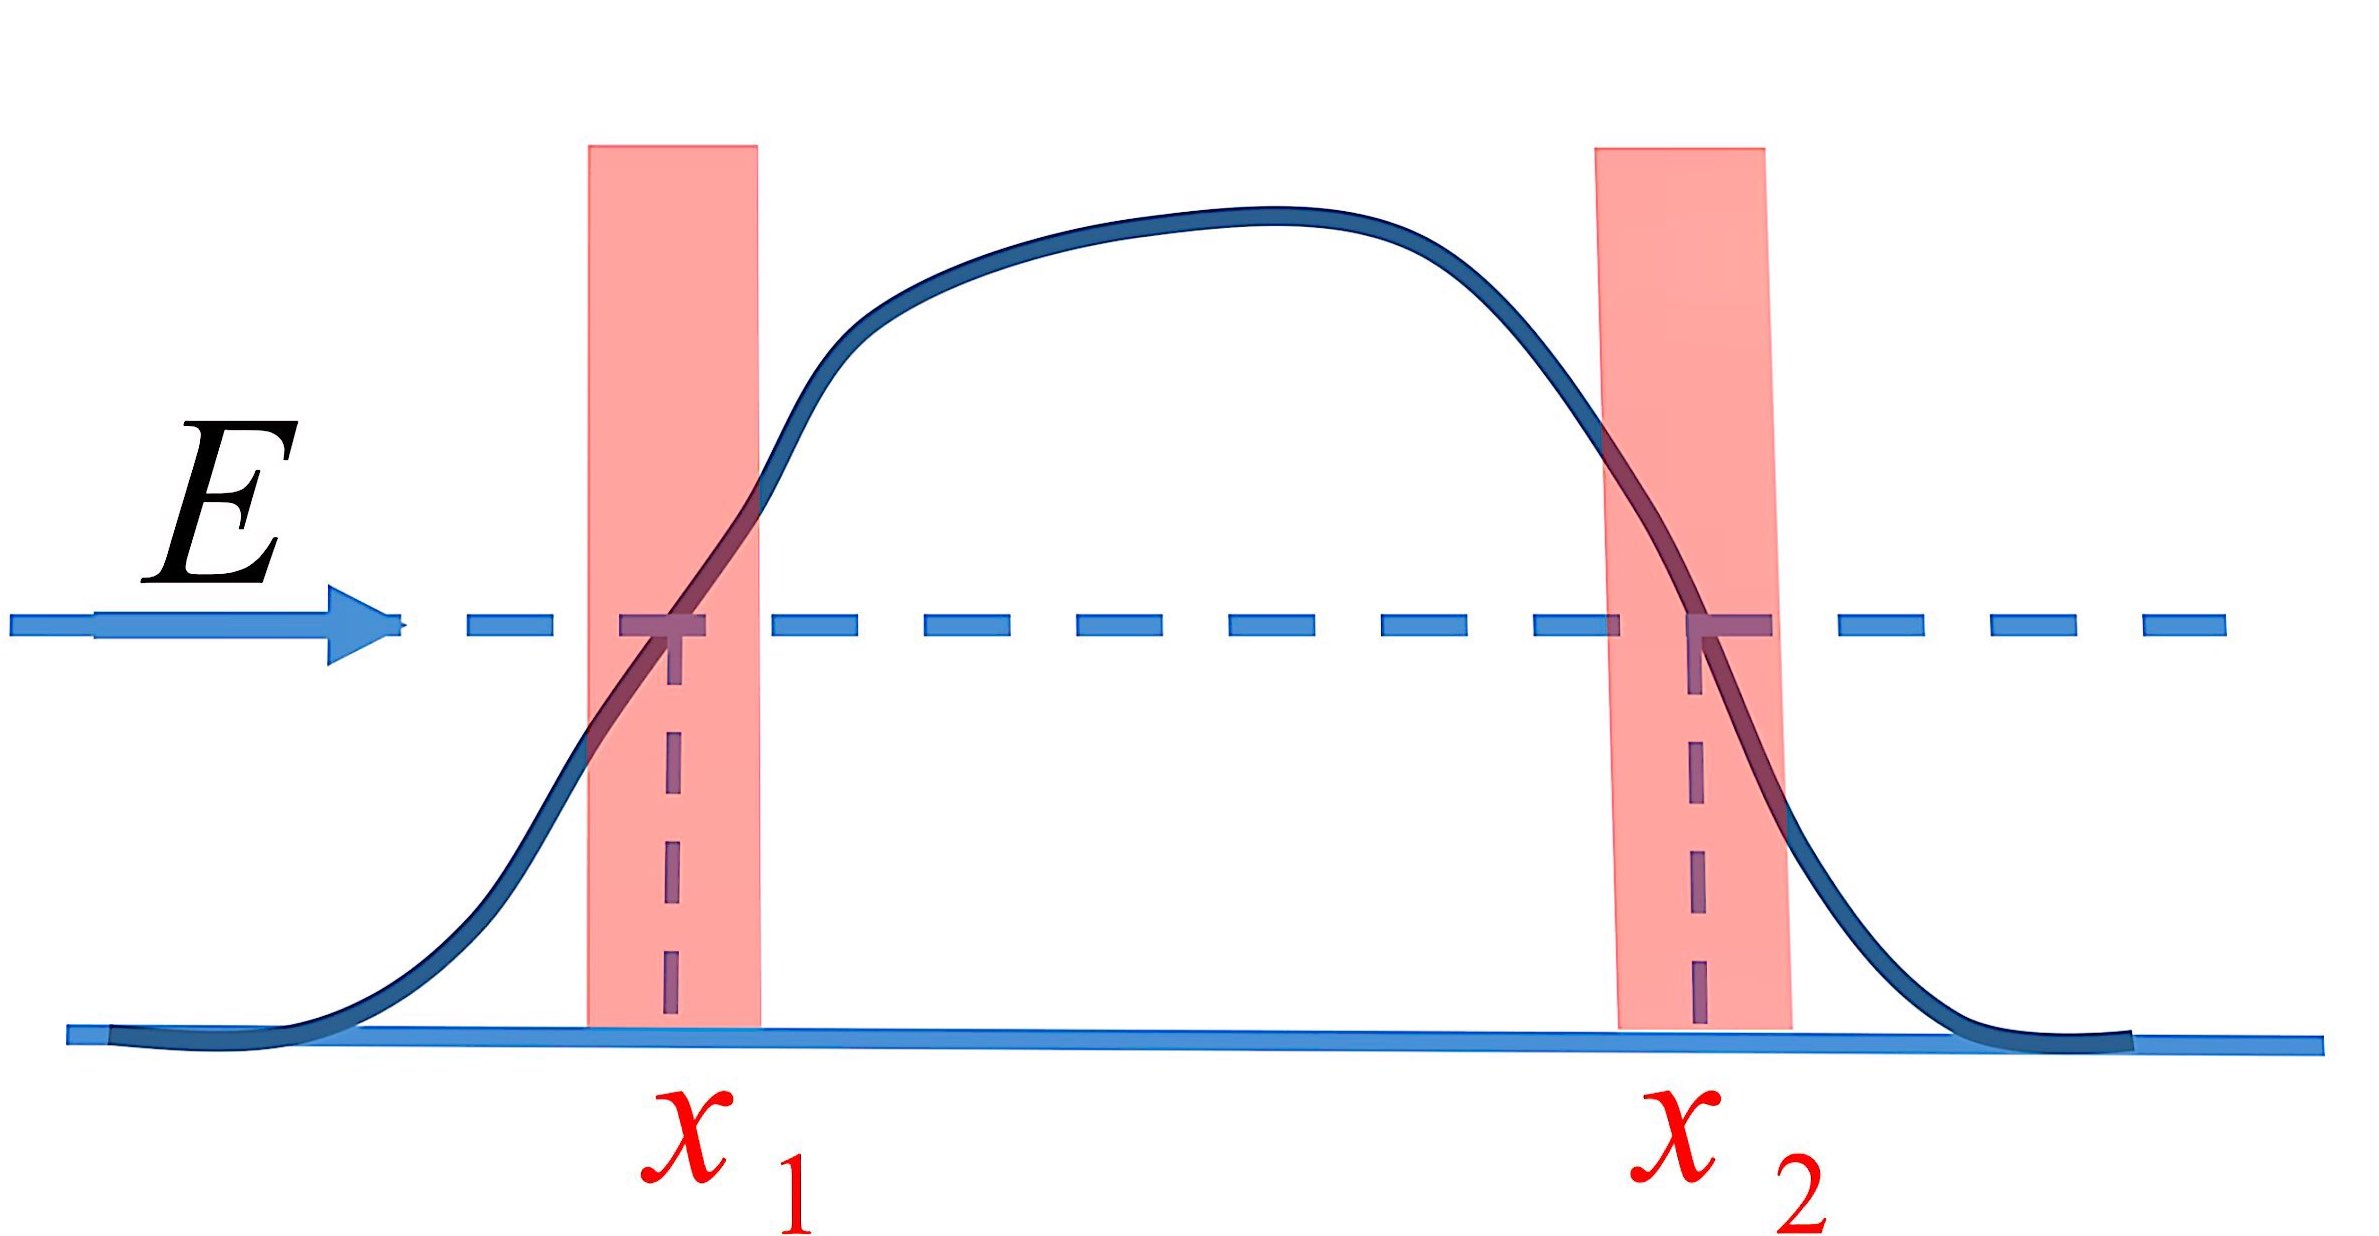
\includegraphics[width=3.5in]{image/WKB_continue_potential_scattering}
          \caption{连续势垒散射应用WKB近似}
        \end{figure}
        不关心修补区, 则体系的波函数形式为:
         \begin{equation}
           \psi_{\mathrm{WKB}} = \left\{\begin{array}{ll}
             \dfrac{A_1}{\sqrt{k(x)}}\mathrm{e}^{i\int_x^{x_1}k(x')\mathrm{d}x'}+%
             \dfrac{A_2}{\sqrt{k(x)}}\mathrm{e}^{-i\int_x^{x_1}k(x')\mathrm{d}x'} & x<x_1\\
             \\
             \dfrac{1}{\sqrt{\alpha(x)}}\left\{B_1\mathrm{e}^{-\int_{x_1}^x\alpha(x')\mathrm{d}x'}+%
                                               B_2\mathrm{e}^{\int_{x_1}^x\alpha(x')\mathrm{d}x'}\right\} & x_1<x< x_2\\
              \\
              \dfrac{C}{\sqrt{k(x)}}\mathrm{e}^{i\int_{x_2^x}k(x')\mathrm{d}x'}, & x>x_2
           \end{array}\right.
         \end{equation}

         为了判断$x_1$左侧区域中的波函数哪一项($A_1$还是$A_2$)是入射波, 需要计算两个部分的流密度算符的期望值.
         
         所谓的流密度算符, 其形式为:
         \begin{equation}
           J_x = \dfrac{-i\hbar}{2m}\left[\psi^*\partial_x\psi-\psi\partial\psi^*\right]
         \end{equation}

         计算系数$A_1$对应的波函数的流密度, 得到:
         \begin{equation}
           (J_x)_{A_1} = \dfrac{-\hbar|A_1|^2}{m}
         \end{equation}

         因此, 系数$A_1$对应的波函数是反射波函数, 则系数$A_2$对应的波函数就是入射波函数. 

         同时, 用入射流密度比上透射流密度来定义透射系数, 可以得到:
         \begin{equation}
           T = \dfrac{|C|^2}{|A_2|^2}
         \end{equation}

         结合上述波函数形式, 利用其在$x_1, x_2$处的连接条件, 易得%
         \footnote{其实就是敲了一天代码, 现在头昏眼花, 啥计算也不想做了...直接给个结果吧, 以后有时间再补上过程@\_@}:
        \begin{equation}
          \begin{aligned}
            A_1 &= \left(-iB_1+\dfrac{B_2}{2}\right)\mathrm{e}^{i\frac{\pi}{4}}\\
            A_2 &= \left(iB_1+\dfrac{B_2}{2}\right)\mathrm{e}^{-i\frac{\pi}{4}}\\
            B_2 &= \dfrac{iB_1}{2}\mathrm{e}^{-2\int_{x_1}^{x_2}\alpha(x')\mathrm{d}x'}\\
            C &=  B_1\dfrac{\pi}{4}\mathrm{e}^{-\int_{x_1}^{x_2}\alpha(x')\mathrm{d}x'}
          \end{aligned}
        \end{equation}

        应用上面对透射系数的定义, 并考虑$\int_{x_1}^{x_2}\alpha(x')\mathrm{d}x'\gg1$的情况%
        \footnote{其实这条件说的就是透射很小的情况, 上面的$B_2$其实可以近似看成是0的, 或者说$B_2$就是0, 因为波函数必须衰减.}:
        \begin{equation}
          \begin{aligned}
            T &= \left|\dfrac{C}{A_2}\right|^2\\
              &= \dfrac{|C|^2}{\left|iB_1+\dfrac{B_2}{2}\right|^2}\\
              &= \dfrac{|B_1|^2\mathrm{e}^{-2\int_{x_1}^{x_2}\alpha(x')\mathrm{d}x'}}%
                 {\left|iB_1+\dfrac{iB_1}{4}\mathrm{e}^{-2\int_{x_1}^{x_2}\alpha(x')\mathrm{d}x'}\right|^2}\\
              &= \dfrac{\mathrm{e}^{-2\int_{x_1}^{x_2}\alpha(x')\mathrm{d}x'}}%
                 {\left|1+\dfrac{1}{4}\mathrm{e}^{-2\int_{x_1}^{x_2}\alpha(x')\mathrm{d}x'}\right|^2}\\
              &\approx \mathrm{e}^{-2\int_{x_1}^{x_2}\alpha(x')\mathrm{d}x'}
          \end{aligned}
        \end{equation}

        这与之前一个例子得到的的透射系数是相同的!

        \textbf{总结上述两个例子, 散射态问题应用WKB近似时, 如果透射几率本身很小, 那么我们认为其透射系数是:}
        \begin{equation}
          T \approx \mathrm{e}^{-2\int_{x_1}^{x_2}\alpha(x')\mathrm{d}x'}
        \end{equation}

        \textbf{是合理的.}
    \section{力学量本征值的代数解法}
      
      力学量本征值的代数解法是一个十分美妙的求解量子力学本征值和本征矢的方法. 我第一次在科恩书上看到这种解法的时候是爱不释手的. 
      下面, 就详细的记录下这种方法的套路. 
      
      \subsection{一维谐振子的代数解法}
      
        观察一维谐振子哈密顿量算符的形式:
        \begin{equation}
          \hat{H} = \dfrac{\hat{p}_x^2}{2m} + \dfrac{1}{2}m\omega^2\hat{x}^2
        \end{equation}

        发现他是两个算符平方相加的形式, 于是我们产生一个奇妙的设想, 能不能将这个哈密顿量算符拆分成一对互为厄米的算符相乘的形式, 
        因为, 互为厄米容易让人们联想到``互为相反操作''这样的概念\footnote{只是脑海中突然蹦出了这么一个词, 也不知道原因是什么}. 
        只是在纸上一试, 应该不会有什么损失. 说得更明白一点就是, 对实数$p, q$有$p^2+q^2=(p+iq)(p-iq)$, 等式右侧的两个因子互为复共轭.
        我们想尝试一下这样的公式放在算符上会不会升级成互为厄米的, 当然还要考虑对易关系:
         $\left[\hat{x}, \hat{p}_x\right] = i\hbar$.

        于是, 我们意外的得到的理想的结果, 如果令算符$\hat{a}$有如下形式: 
        \begin{equation}
          \label{4120:a}
          \hat{a} = \dfrac{1}{\sqrt{2}}\left(\sqrt{\dfrac{m\omega}{\hbar}}\hat{x}+%
                    \dfrac{i\hat{p}_x}{\sqrt{m\hbar\omega}}\right)
        \end{equation}

        那么就会有:
        \begin{equation}
          \label{4120:adagger}
          \hat{a}^{\dagger} = \dfrac{1}{\sqrt{2}}\left(\sqrt{\dfrac{m\omega}{\hbar}}\hat{x}-%
                              \dfrac{i\hat{p}_x}{\sqrt{m\hbar\omega}}\right)
        \end{equation}
        
        上述构造的新算符内部之所以有看似十分复杂的系数, 是因为我们想用$\hat{a}$化简哈密顿量算符, 并使之在形式上更加简洁. 于
        是对$\hat{a}$的去量纲化是必然的. 将$\hat{a}$与$\hat{a}^{\dagger}$带入原哈密顿量算符可得:
        \begin{equation}
          \hat{H} = \hbar\omega\hat{a}^{\dagger}\hat{a}+\dfrac{1}{2}\hbar\omega
        \end{equation}

        到这里, 如果洞察力足够, 那么应该感到上述结果是十分和谐的! 或者对于强迫症患者们来说, 上式还是不够简洁, 于是我们再构
        造一个算符$\hat{n}\equiv\hat{a}^{\dagger}\hat{a}$, 上式进一步化简为:
        \begin{equation}
          \hat{H} = \left(\hat{n}+\dfrac{1}{2}\right)\hbar\omega
        \end{equation}

        这真是令人眼前一亮的结果, 他和一维谐振子的本征能量表达式的区别仅仅是将算符$\hat{n}$换为非负整数$n$而已. 

        现在的关键问题在于求解算符$\hat{n}$的本征矢和本征值. 因为$\hat{H}$与$\hat{n}$具有相同的本征矢, 本征值的关系
        也包含在上式当中. 甚至有理由相信, $\hat{n}$的本征值就是非负整数$n$.
        
        因此, 我们需要对算符$\hat{n}$有更近一步的认识.  

        首先, 需要先引入一些约定, 若有关系:
        \begin{equation}
          \hat{n}|\varphi_{\varepsilon}\rangle = \varepsilon|\varphi_{\varepsilon}\rangle
        \end{equation}
      
        则将$|\varphi_{\varepsilon}\rangle$简写作$|\varepsilon\rangle$

        定义\textbf{阶},\textbf{降阶}和\textbf{升阶}概念. 声称: 本征矢$|\varepsilon\rangle$处在
        $\varepsilon$阶上, $|\varepsilon-m\rangle$是相对于本征矢$|\varepsilon\rangle$
        降了$m$阶, 升阶类似.\footnote{这个地方的定义完全是我一时兴起.}

        经过一些探索, 我们得到了如下结论:

        \textbf{1. 算符$\hat{n}$的本征值$\varepsilon$一定是非负数.}

        对此结论的证明是简单的: 
        \begin{equation}
          \varepsilon = \langle\varepsilon|\hat{n}|\varepsilon\rangle %
                      = \langle\varepsilon|\hat{a}^{\dagger}\hat{a}|\varepsilon\rangle%
                      = \big|\big|\hat{a}|\varepsilon\rangle\big|\big|^2 \geq 0
        \end{equation}

        \textbf{2. 算符$\hat{a}^{\dagger}$的作用是将$\hat{n}$的本征矢升1阶}\footnote{这么一看算符后面加一个
        dagger似乎很形象!}

        证明这上述结论之前, 需要计算一些相关的对易式:

        如果计算能力扎实, 以下的结论将是显然的:
        \begin{subequations}
          \begin{align}
            \left[\hat{a}, \hat{a}^{\dagger}\right] &= 1\\
            \left[\hat{n}, \hat{a}\right] &= -\hat{a}\\
            \left[\hat{n}, \hat{a}^{\dagger}\right] &= \hat{a}^{\dagger}\\
            \left[\hat{n}, \hat{a}^m\right] &= -m\hat{a}^m\\
            \left[\hat{n}, \left(\hat{a}^{\dagger}\right)^m\right] &= m\left(\hat{a}^{\dagger}\right)^m
          \end{align}
        \end{subequations}

        利用上面的对易式, 计算这样一个式子:
        \begin{equation}
          \hat{n}\hat{a}^{\dagger}|\varepsilon\rangle = (\hat{a}^{\dagger}\hat{n}+\hat{a}^{\dagger})|\varepsilon\rangle%
          = (\varepsilon+1)\hat{a}^{\dagger}|\varepsilon\rangle
        \end{equation}

        因此, $\hat{a}^{\dagger}|\varepsilon\rangle$就可以视为是$c_{\varepsilon}^{+}|\varepsilon+1\rangle$, 
        其中$c_{\varepsilon}^{+}$是归一化系数. 

        \textbf{3. 算符$\hat{a}$的作用是将$\hat{n}$的本征矢降1阶, 但除了$|0\rangle$之外.}

        计算这一规律的套路和上面是类似的. 

        利用之前的对易式: 
        \begin{equation}
          \hat{n}\hat{a}|\varepsilon\rangle = (\hat{a}\hat{n}-\hat{a})|\varepsilon\rangle%
          = (\varepsilon-1)\hat{a}|\varepsilon\rangle
        \end{equation}

        因此, $\hat{a}|\varepsilon\rangle$就可以视为是$c_{\varepsilon}^{-}|\varepsilon-1\rangle$, 
        其中$c_{\varepsilon}^{-}$是归一化系数.

        但要注意, 如果把$\varepsilon=0$带入上述方程, 可以得到:
        \begin{equation}
          \hat{n}\hat{a}|0\rangle = (\hat{a}\hat{n}-\hat{a})|0\rangle%
          = -\hat{a}|0\rangle
        \end{equation}

        这貌似就是在说,$\hat{a}|0\rangle$就是$c_{0}^{-}|-1\rangle$. 但是, 如果再在这个本征矢上作用上一个$\hat{a}^{\dagger}$
        就会发现问题. 

        如果认为$\hat{a}|0\rangle$就是$c_{0}^{-}|-1\rangle$, 那么, 作用一个$\hat{a}^{\dagger}$后, 方程变为:
        \begin{equation}
          \hat{a}^{\dagger}\hat{a}|0\rangle = \hat{a}^{\dagger}c_{0}^{-}|-1\rangle %
              = c_{-1}^{+}c_{0}^{-}|0\rangle
        \end{equation}

        另一方面:
        \begin{equation}
          \hat{a}^{\dagger}\hat{a}|0\rangle = \hat{n}|0\rangle = 0
        \end{equation}

        由于$c_{-1}^{+}c_{0}^{-}$是归一化系数, 不为0 , 于是我们得到:
        \begin{equation}
          |0\rangle = 0
        \end{equation}

        这显然是错误的!

        这个错误的引起貌似是由于$|0\rangle$这个态的本征值太特殊导致的, 于是我们先声明\textbf{结论3}对于$|0\rangle$态是不成立的. 
        之后再仔细分析这个问题. 

        \textbf{4. 算符$\hat{a}$的作用在$|0\rangle$这个态上会得到0}

        现在仔细分析上面得到一个矛盾和错误, 观察之前得到的这个等式:
        \begin{equation*}
        \hat{n}\hat{a}|0\rangle = (\hat{a}\hat{n}-\hat{a})|0\rangle = -\hat{a}|0\rangle
        \end{equation*}

        发现这样一个事实, 如果$\hat{a}|0\rangle\equiv0$, 这个方程也是成立的!

        事实是否如此呢?
        \begin{equation}
          0 = \langle0|\hat{n}|0\rangle = \langle0|\hat{a}^{\dagger}\hat{a}|0\rangle = %
          \big|\big|\hat{a}|0\rangle\big|\big|^2
        \end{equation}

        一个向量的模是$0$, 那么就有$\hat{a}|0\rangle = 0$

        事实正是如此!

        \textbf{得到上述四个结论后, 就可以开始分析了:}
        首先我们称, $\hat{a}$为降算符(湮灭算符), $\hat{a}^{\dagger}$为升算符(产生算符). 这是很形象的命名!

        同时注意到, 上面四个结论没有因果关系, 他们是相互独立成立的. 也就是, 他们必须同时被满足. 因此, 如果一个随便取一个态
        $|\varepsilon\rangle$, 对他一直作用$\hat{a}$算符, 总会使之变为本征值为负数的本征态, 但这是结论1所不允许的!
        
        但是, 所有的结论和分析过程都没有错, 那为何最后会推出两个结论之间的矛盾呢? 只能是我们的初始条件选取有问题. 也就是不能
        随便选取本征值为任意值的本征矢. 此时, 我们想起了结论4和之前的对$\hat{n}$本征值的预言, 
        机智的声称:$\varepsilon$只能选取非负整数$n$. 

        这样, 由于在$|0\rangle$处的``截断''效应, 一切矛盾都消失了. 整个理论体系变得十分和谐.

        \textbf{于是, 最终的结论就是:算符$\hat{n}$的本征值是非负整数$n$. 本征矢是$|n\rangle$. 进而, 一维谐振子哈密顿量
        本征值是$E_n = \left(n+\dfrac{1}{2}\right)\hbar\omega, (n=0,1,2,\ldots)$,本征矢是$|n\rangle$.}

        至此, 我们基本解出了想要的结果, 然而还有几个后续问题需要解决:\textbf{1,归一化系数是多少? 2,升降算符
        到底是长什么样的,有没有直观一点的表示? 3,怎么得到本征矢在坐标表象下的形式,也就是波函数?}

        下面一一解决这些问题:
        
        \textbf{1. 归一化系数的求解}

        这个问题的求解是简单的, 按如下套路操作即可:

        先取定一个归一化完毕的基态$|0\rangle$. 而后归一化的各个态就可写作:
        \begin{equation}
          \begin{aligned}
            &|1\rangle = c_0^+\hat{a}^{\dagger}|0\rangle\\
            &|2\rangle = c_1^+\hat{a}^{\dagger}|1\rangle\\
            &\ldots\\
            &|n\rangle = c_{n-1}^+\hat{a}^{\dagger}|n-1\rangle\\
          \end{aligned}
        \end{equation}
        
        利用之前求得的
        $[\hat{a}, \hat{a}^{\dagger}]$的对易关系, 可得:
        \begin{equation}
          \begin{aligned}
            1 &= \langle1|1\rangle = \left(c_0^+\right)^2\langle0|\hat{a}\hat{a}^{\dagger}|0\rangle%
            = \left(c_0^+\right)^2\langle0|1+\hat{a}^{\dagger}\hat{a}|0\rangle\\
            &= \left(c_0^+\right)^2\langle0|1+\hat{n}|0\rangle
            = \left(c_0^+\right)^2\\
            1 &= \langle2|2\rangle = \left(c_1^+\right)^2\langle1|\hat{a}\hat{a}^{\dagger}|1\rangle%
            = \left(c_1^+\right)^2\langle1|1+\hat{a}^{\dagger}\hat{a}|1\rangle\\
            &= \left(c_1^+\right)^2\langle1|1+\hat{n}|1\rangle
            = 2\left(c_1^+\right)^2\\
            &\ldots\\
            1 &= \langle{}n|n\rangle = \left(c_{n-1}^+\right)^2\langle{}n-1|\hat{a}\hat{a}^{\dagger}|n-1\rangle%
            = \left(c_{n-1}^+\right)^2\langle{}n-1|1+\hat{a}^{\dagger}\hat{a}|n-1\rangle\\
            &= \left(c_{n-1}^+\right)^2\langle{}n-1|1+\hat{n}|n-1\rangle
            = n\left(c_{n-1}^+\right)^2\\
          \end{aligned}
        \end{equation}

        从而得到:
        \begin{equation}
          \label{4316:dd1}
          |n\rangle = \dfrac{1}{\sqrt{n}}\hat{a}^{\dagger}|n-1\rangle
        \end{equation}

        这是一个关于$\hat{a}^{\dagger}$递推关系式.

        利用类似的套路, 同样是设有一个归一化的基态$|0\rangle$, 就可以得到$\hat{a}$的递推关系式.
        \begin{equation}
          \label{4316:dd2}
          |n\rangle = \dfrac{1}{\sqrt{n+1}}\hat{a}|n+1\rangle
        \end{equation}

        至此, 我们解决了归一化系数问题. 

        \textbf{2. 升降算符的形式}

        如果将升降算符在能量本征值下矩阵表示. 那么, 无非就是求解下面两个表达式:
        \begin{equation}
          \label{pxdsjf}
          \begin{aligned}
            &\langle{}m|\hat{a}|n\rangle \\
            &\langle{}m|\hat{a}^{\dagger}|n\rangle\\
            &m,n=0,1,2,\ldots 
          \end{aligned}
        \end{equation}

        将\eqref{4316:dd1}与\eqref{4316:dd2}带入上式可得到升降算符的矩阵形式为:
        \begin{equation}
          \begin{aligned}
          \hat{a} &= 
          \begin{bmatrix}
            0      & \sqrt{1} & 0        & 0       &\ldots \\
            0      & 0        & \sqrt{2} & 0       &\ldots \\
            0      & 0        & 0        & \sqrt{3}&\ldots \\
            0      & 0        & 0        & 0       &\ldots \\
            \vdots & \vdots   & \vdots   & \vdots  &\ddots \\
          \end{bmatrix}\\[4pt]
          \hat{a}^{\dagger} &= 
          \begin{bmatrix}
            0       & 0        & 0        & 0       &\ldots \\
            \sqrt{1}& 0        & 0        & 0       &\ldots \\
            0       & \sqrt{2} & 0        & 0       &\ldots \\
            0       & 0        & \sqrt{3} & 0       &\ldots \\
            \vdots  & \vdots   & \vdots   & \vdots  &\ddots \\
          \end{bmatrix}\\
          \end{aligned}
        \end{equation}

        参考升降算符的形式\eqref{4120:a}与\eqref{4120:adagger}, 可得:
        \begin{equation}
          \begin{aligned}
            \hat{x} = \sqrt{\dfrac{\hbar}{2m\omega}}\left(\hat{a}+\hat{a}^{\dagger}\right)&\\
            \hat{p}_x = -i\sqrt{\dfrac{m\omega\hbar}{2}}\left(\hat{a}-\hat{a}^{\dagger}\right)&
          \end{aligned}
        \end{equation}

        将升降算符的矩阵形式带入上式得:
        \begin{equation}
          \begin{aligned}
          \hat{x} &= \sqrt{\dfrac{\hbar}{2m\omega}}
          \begin{bmatrix}
            0       & \sqrt{1} & 0        & 0       &\ldots \\
            \sqrt{1}& 0        & \sqrt{2} & 0       &\ldots \\
            0       & \sqrt{2} & 0        & \sqrt{3}&\ldots \\
            0       & 0        & \sqrt{3} & 0       &\ldots \\
            \vdots  & \vdots   & \vdots   & \vdots  &\ddots \\
          \end{bmatrix}\\[4pt]
          \hat{p}_x &= -i\sqrt{\dfrac{m\omega\hbar}{2}}
          \begin{bmatrix}
            0        & \sqrt{1} & 0        & 0       &\ldots \\
            -\sqrt{1}& 0        & \sqrt{2} & 0       &\ldots \\
            0        & -\sqrt{2}& 0        & \sqrt{3}&\ldots \\
            0        & 0        & -\sqrt{3}& 0       &\ldots \\
            \vdots   & \vdots   & \vdots   & \vdots  &\ddots \\
          \end{bmatrix}\\
          \end{aligned}
        \end{equation}
        
        显然, 上述两个矩阵是厄米的\footnote{系数也是矩阵的一部分\ldots}. 
        而且由于其对角元均为$0$, 因此可以判断$\hat{x}$和$\hat{p}_x$
        两个力学量关于能量本征态的期望是$0$.

        \textbf{3. 能量本征波函数的求解}

        由递推关系式\eqref{4316:dd1}, 可以得到:
        \begin{equation}
          \label{4407:nn}
          |n\rangle = \dfrac{1}{\sqrt{n!}}\left(\hat{a}^{\dagger}\right)^n|0\rangle
        \end{equation}

        其中, $n=1,2,3,\ldots$

        同时$\hat{a}^{\dagger}$与$\hat{a}$在坐标表象下的形式可由$\hat{x}, \hat{p}_x$推出, 具体的:

        首先求$\hat{a}^{\dagger}$
        \begin{equation}
          \begin{aligned}
            \hat{a}^{\dagger} &= \dfrac{1}{\sqrt{2}}\left(\sqrt{\dfrac{m\omega}{\hbar}}\hat{x}-%
            \dfrac{i\hat{p}_x}{\sqrt{m\hbar\omega}}\right)\\
            &\overset{|\xi\rangle}{=} \dfrac{1}{\sqrt{2}}\left(\sqrt{\dfrac{m\omega}{\hbar}}x-%
            \sqrt{\dfrac{\hbar}{m\omega}}\dfrac{\partial}{\partial{}x}\right)\\
          \end{aligned}
        \end{equation}

        同理, 对$\hat{a}$:
        \begin{equation}
          \begin{aligned}
            \hat{a}&= \dfrac{1}{\sqrt{2}}\left(\sqrt{\dfrac{m\omega}{\hbar}}\hat{x}+%
            \dfrac{i\hat{p}_x}{\sqrt{m\hbar\omega}}\right)\\
            &\overset{|\xi\rangle}{=} \dfrac{1}{\sqrt{2}}\left(\sqrt{\dfrac{m\omega}{\hbar}}x+%
            \sqrt{\dfrac{\hbar}{m\omega}}\dfrac{\partial}{\partial{}x}\right)\\    
          \end{aligned}
        \end{equation}
        
        因此, 有了\eqref{4407:nn}, 求解一维谐振势全部本征波函数的问题就转化为了, 如
        何求解$|0\rangle$在$|\xi\rangle$表象, 也即坐标表象, 下的形式. 
        
        有前面的分析可知, 有关系:
        \begin{equation}
          \hat{a}|0\rangle = 0
        \end{equation}

        也即:
        \begin{equation}
          \dfrac{1}{\sqrt{2}}\left(\sqrt{\dfrac{m\omega}{\hbar}}x+%
          \sqrt{\dfrac{\hbar}{m\omega}}\dfrac{\partial}{\partial{}x}\right)\psi_0(x) = 0
        \end{equation}

        求解上述方程, 可得到
        \begin{equation}
          \psi_0(x) = \left(\dfrac{m\omega}{\pi\hbar}\right)^{\frac{1}{4}}%
          \mathrm{e}^{-\frac{1}{2}\frac{m\omega}{\hbar}x^2}
        \end{equation}
        
        进而, 
        \begin{equation}
          \begin{aligned}
            \psi_n(x) &= \dfrac{1}{\sqrt{n!}}\left(\hat{a}^{\dagger}\right)^n|0\rangle\\
            &= \dfrac{1}{\sqrt{2^nn!}}\left(\sqrt{\dfrac{m\omega}{\hbar}}x-%
            \sqrt{\dfrac{\hbar}{m\omega}}\dfrac{\partial}{\partial{}x}\right)^n\psi_0(x)\\
            &= \left(\dfrac{m\omega}{\pi\hbar}\right)^{\frac{1}{4}}%
            \dfrac{1}{\sqrt{2^nn!}}\left(\sqrt{\dfrac{m\omega}{\hbar}}x-%
            \sqrt{\dfrac{\hbar}{m\omega}}\dfrac{\partial}{\partial{}x}\right)^n%
            \mathrm{e}^{-\frac{1}{2}\frac{m\omega}{\hbar}x^2}\\
            &(n=1,2,3,\ldots)
          \end{aligned}
        \end{equation}

        总结整理基态波函数和激发态波函数的形式, 可得到:
        \begin{equation}
          \begin{aligned}
            \psi_n(x)&= \left(\dfrac{m\omega}{\pi\hbar}\right)^{\frac{1}{4}}%
            \dfrac{1}{\sqrt{2^nn!}}\left(\sqrt{\dfrac{m\omega}{\hbar}}x-%
            \sqrt{\dfrac{\hbar}{m\omega}}\dfrac{\partial}{\partial{}x}\right)^n%
            \mathrm{e}^{-\frac{1}{2}\frac{m\omega}{\hbar}x^2}\\
            &(n=0,1,2,\ldots)
          \end{aligned}
        \end{equation}

        至此, 我们讨论了一维谐振子问题的代数解法. 

        \textbf{讨论两个具体的例子以加深对上述论证的理解.}

        \emph{1. 计算均匀带电场中电荷谐振子的能级}

        \emph{设电荷电量为$q$, 质量为$m$. 在均匀外场$\varepsilon$的作用下. 求解该体系的能量本征值.}

        此体系的哈密顿量显然为:
        \begin{equation}
          \hat{H} = \dfrac{\hat{p}^2}{2m}+\dfrac{1}{2}m\omega^2\hat{x}^2-q\varepsilon\hat{x}
        \end{equation}

        利用\eqref{pxdsjf}中的第一式, 即
        \begin{equation*}
          \hat{x} = \sqrt{\dfrac{\hbar}{2m\omega}}\left(\hat{a}+\hat{a}^{\dagger}\right)
        \end{equation*}

        可将上述哈密顿量转换为如下形式:
        \begin{equation}
          \begin{aligned}
            \hat{H} &= \left[\hat{a}^{\dagger}\hat{a}+\dfrac{1}{2}-\alpha_0\left(\hat{a}^{\dagger}%
            +\hat{a}\right)\right]\hbar\omega\\
            \alpha_0 &\equiv \dfrac{q\varepsilon}{\omega}\sqrt{\dfrac{1}{2m\hbar\omega}}
          \end{aligned}
        \end{equation}

        为了进一步化简上述形式的哈密顿量, 定义新的算符$\hat{b} = \hat{a}-\alpha_0$, 那么显然有:
        $\hat{b}^{\dagger} = \hat{a}^{\dagger} - \alpha_0$. 并且, $[\hat{b}, \hat{b}^{\dagger}] = 1$.
        事实上, 经过简单的推导就可以发现, $\hat{a}$与$\hat{b}$满足相同的对易性质. 

        进而, $\hat{H}$可表示为:
        \begin{equation}
          \hat{H} = \left[\hat{b}^{\dagger}\hat{b}+\dfrac{1}{2}-\alpha_0^2\right]\hbar\omega
        \end{equation}

        因此, 体系的本征能量为:
        \begin{equation}
          E_n = \left(n+\dfrac{1}{2}\right)\hbar\omega-\dfrac{q^2\varepsilon^2}{2m\omega^2}, \qquad(n=0,1,2,\ldots)
        \end{equation} 

        求解此体系$\hat{x}$算符的平均值:
        \begin{equation}
          \begin{aligned}
            \langle{}n|\hat{x}|n\rangle &= \langle{}n|\sqrt{\dfrac{\hbar}{2m\omega}}
                                   \left(\hat{a}+\hat{a}^{\dagger}\right)|n\rangle \\
                                   &= \sqrt{\dfrac{\hbar}{2m\omega}}\langle{}n|
                                   \left(\hat{b}+\hat{b}^{\dagger}+2\alpha_0\right)|n\rangle\\
                                   &= \sqrt{\dfrac{\hbar}{2m\omega}}\langle{}n|
                                   2\alpha_0|n\rangle\\
                                   &= \dfrac{q\varepsilon}{m\omega^2}
          \end{aligned}
        \end{equation}

        这是十分直观的物理图像. 粒子振动平衡位置因电场的存在而偏移了$\dfrac{q\varepsilon}{m\omega^2}$的距离!

        \emph{2. 计算一种二维石墨烯材料}
        
        \emph{描述一种二维石墨烯材料的低能有效哈密顿量可写为:}
        \begin{equation}
          \hat{H} = \gamma\vec{\hat{\sigma}}\cdot\vec{\hat{p}} = %
          \gamma\left(\sigma_xp_x+\sigma_yp_y\right)
        \end{equation}
        \emph{其中, $\sigma_x$和$\sigma_y$为Pauli矩阵, $p_x, p_y$为电子动量算符的$x,y$分量. 若对该体系施加沿着
        $z$方向的均匀磁场$\vec{B}=(0,0,B)$, 求该二维体系的Landau能级.}

        选择Landau规范, 磁矢势$\vec{A} = (-By, 0, 0)$. 引入磁场后, 体系的机械动量和正则动量形式不再相同. 

        具体的:
        \begin{equation}
          \vec{\hat{\pi}} = \vec{\hat{p}} - q\vec{A} 
        \end{equation}

        而上述哈密顿量中的动量显然应为机械动量\footnote{对于知道上述哈密顿量的来源的人, 这个结论是显然的; 对于
        不知道这个哈密顿量怎么来的, 只是当黑箱用的人, 也是显然的, 因为这并不会影响黑箱的使用.}. 

        因此原哈密顿量变为:
        \begin{equation}
          \begin{aligned}
            \hat{H} &= \hbar\gamma\left[\sigma_x\left(\hat{k}_x+\dfrac{qB\hat{y}}{c\hbar}\right)%
            +\sigma_y\hat{k}_y\right] \\
            &=\hbar\gamma%
            \begin{bmatrix}
              0        & \left(\hat{k}_x-\dfrac{eB\hat{y}}{c\hbar}\right)-i\hat{k}_y  \\
              \left(\hat{k}_x-\dfrac{eB\hat{y}}{c\hbar}\right)+i\hat{k}_y & 0         \\
            \end{bmatrix}\\
          \end{aligned}
        \end{equation}
        
        对于上述哈密顿量, 显然有:
        \begin{equation}
          \begin{aligned}
            \left[\hat{H}, \hat{k}_x\right] &= 0\\
            \left[\hat{H}, \hat{k}_y\right] &\ne 0
          \end{aligned}
        \end{equation}

        这意味着体系的$\hat{k}_x$是守恒量, 或者说, 体系的$k_x$将一直处在某一个特定的数值上. 因此, 
        该数值对应的量子态显然为$\mathrm{e}^{ik_xx}$. 注意到由于$\hat{k}_x$是守恒量, 因此我们甚至
        可以直接把式子中的算符换成数值\footnote{也就是把$k_x$的帽子去掉}. 

        于是此哈密顿量对应的定态Schr\"odinger方程可写为:
        \begin{equation}
          \begin{aligned}
            \hbar\gamma
            \begin{bmatrix}
              0        & \left(k_x-l_B^{-2}\hat{y}\right)-i\hat{k}_y  \\
              \left(k_x-l_B^{-2}\hat{y}\right)+i\hat{k}_y & 0         \\
            \end{bmatrix}
            &\left(\begin{array}{c}
              \varphi_a(y)\\
              \varphi_b(y)
            \end{array}\right)
            \mathrm{e}^{ik_xx}\\ 
            = E&\left(\begin{array}{c}
              \varphi_a(y)\\
              \varphi_b(y)
            \end{array}\right)\mathrm{e}^{ik_xx} \\
          \end{aligned}
        \end{equation}
        
        其中, $l_B \equiv \sqrt{\dfrac{c\hbar}{eB}}$

        下面引入产生湮灭算符:
        \begin{subequations}
          \begin{align}
            \hat{a} &= \dfrac{1}{\sqrt{2}}\left[\dfrac{\hat{y}-l_B^2k_x}{l_B}+il_B\hat{k}_y\right]\\
            \hat{a}^{\dagger} &= \dfrac{1}{\sqrt{2}}\left[\dfrac{\hat{y}-l_B^2k_x}{l_B}-il_B\hat{k}_y\right]
          \end{align}
        \end{subequations}

        耐心计算上述两个算符的对易式就会得到:
        \begin{equation}
          \label{szjf:gjdys}
          \left[\hat{a}, \hat{a}^{\dagger}\right] = 1
        \end{equation}

        用上述引入的产生湮灭算符简化原定态Schr\"odinger方程:
        \begin{equation}
          \label{szjf:xt2:h}
            \hbar\gamma
            \begin{bmatrix}
              0        & -\dfrac{\sqrt{2}}{l_B}\hat{a}  \\
              -\dfrac{\sqrt{2}}{l_B}\hat{a}^{\dagger} & 0         \\
            \end{bmatrix}
            \left(\begin{array}{c}
              \varphi_a\\
              \varphi_b
            \end{array}\right)
            = E\left(\begin{array}{c}
              \varphi_a\\
              \varphi_b
            \end{array}\right)
        \end{equation}

        由于$x$分量的波函数是显然的, 因此方程中只保留了$y$分量的波函数形式. 

        由上述方程组可推出如下等式:
        \begin{equation}
          \left(\hbar\gamma\dfrac{\sqrt{2}}{l_B}\right)^2\hat{a}^{\dagger}\hat{a}\varphi_b = %
          -\hbar\gamma\dfrac{\sqrt{2}}{l_B}\hat{a}^{\dagger}E\varphi_a = %
          E^2\varphi_b
        \end{equation}

        由于算符$\hat{a}$满足\eqref{szjf:gjdys}式, 因此, 有:
        \begin{equation}
          \hat{a}^{\dagger}\hat{a}|n\rangle = \hat{n}|n\rangle = n|n\rangle%
          \qquad (n=0,1,2,\ldots)
        \end{equation} 

        进而:
        \begin{equation}
          \label{Dirac:ele}
          \begin{aligned}
            E &= \pm\dfrac{\sqrt{2}\hbar\gamma}{l_B}\sqrt{n}\\
            l_B &\equiv \dfrac{c\hbar}{eB}\\
            n &= 0,1,2,\ldots 
          \end{aligned}
        \end{equation}

        另外, 从\eqref{szjf:xt2:h}可以得到, $a$分量上的波函数比$b$分量上的波函数低一
        阶\footnote{阶的定义在之前提到过}. 而具体每一阶的波函数怎么求, 可以参考之前一维谐振子的求解方法. 
        得到$y$分量的波函数后, 只需再乘上$x$分量的波函数, 就可以得到最终的波函数. 
        对于此体系波函数的问题, 这里就不再赘述.

        \textbf{如果仔细品味一维谐振子的力学量本征值数值解法, 就不难发现, 这个方法
        全部的精妙的源头就蕴含在一个小小的对易式里:}
        \begin{equation}
          \mathbf{
          \left[\hat{a}, \hat{a}^{\dagger}\right] = 1}
        \end{equation}
        
        \textbf{其他全部的妙不可言的性质都来自于这个简单的对易式. }

      \subsection{角动量的本征问题}

      \textbf{角动量问题是量子力学中一个非常非常非常非常重要的问题. 而角动量力学量本征值的数值解法, 和之前的一维谐振子
      在构造和对易关系本质上又会有所不同. 因此有必要单独说明.}
      
      量子力学中角动量的本质可用如下等式阐明:
      \begin{equation}
        \left[\hat{J}_{\alpha}, \hat{J}_{\beta}\right] = %
        i\hbar\varepsilon_{\alpha\beta\gamma}\hat{J}_{\gamma}
      \end{equation}

      式中的$\varepsilon_{\alpha\beta\gamma}$被称为三阶反对称张量, 其具体而繁琐的定义为:
      若其下标中的指标是顺序排列, 则其值为$1$; 若有相同下标其值为$0$; 其他情况下, 其值为$-1$.
      所谓下标的顺序, 是先由右手螺旋法则确定空间坐标轴$xyz$(或称为$x_1, x_2, x_3$, 随便你怎么称呼)的指向后, 
      再将满足$xyz, zxy, yzx$的下标排列称为顺序排列. 可以看到, 这个定义本身就包含了角动量的
      特殊的空间结构特征. 

      或者, 可以用一个$(3\times3\times3)$的三维``矩阵''十分简单的定义这个符号. 
      这样一来, 所谓的三阶反对称张量, 就名符其实了. 
      
      可以证明, 上述对角动量的定义和下列的式子是等价的:
      \begin{equation}
        \label{4723:zzsz}
        \left\{
          \begin{aligned}
            &\hat{J}^2|jm\rangle = j(j+1)\hbar^2|jm\rangle\\
            &\hat{J}_z|jm\rangle = m\hbar|jm\rangle \\
            &j = 0,1,2,\ldots \quad or \quad j=\frac{1}{2}, \dfrac{3}{2}, \dfrac{5}{2}, \ldots\\
            &m = -j, -j+1, \ldots, j-1, j
          \end{aligned}\right.
      \end{equation}

      应该明确, $\hat{J}^2 = \hat{J}_x^2+\hat{J}_y^2+\hat{J}_z^2$

      下面证明上述结论. 

      引入角动量的升降算符:
      \begin{subequations}
        \begin{align}
          \hat{J}_- = \hat{J}_x-i\hat{J}_y&\\
          \hat{J}_+ = \hat{J}_-^{\dagger} =  \hat{J}_x+i\hat{J}_y&
        \end{align}
      \end{subequations}

      应该有等式:
      \begin{subequations}
        \begin{align}
          \begin{aligned}
            \hat{J}_+\hat{J}_- &= \left(\hat{J}_x+i\hat{J}_y\right)\left(\hat{J}_x-i\hat{J}_y\right)\\
                               &= \hat{J}_x^2+\hat{J}_y^2-i\left[\hat{J}_x,\hat{J}_y\right]\\
                               &= \hat{J}_x^2+\hat{J}_y^2+\hbar\hat{J}_z\\
                               &= \hat{J}^2 - \hat{J}_z^2+\hbar\hat{J}_z
          \end{aligned}\\
          \begin{aligned}
            \hat{J}_-\hat{J}_+ &= \left(\hat{J}_x-i\hat{J}_y\right)\left(\hat{J}_x+i\hat{J}_y\right)\\
                               &= \hat{J}_x^2+\hat{J}_y^2+i\left[\hat{J}_x,\hat{J}_y\right]\\
                               &= \hat{J}_x^2+\hat{J}_y^2-\hbar\hat{J}_z\\
                               &= \hat{J}^2-\hat{J}_z^2- \hbar\hat{J}_z
          \end{aligned}
        \end{align}
      \end{subequations}

      以下的对易式将是显然的:
      \begin{subequations}
        \label{4764:ee}
        \begin{align}
          &\left[\hat{J}^2, \hat{J}_{z}\right] = 0 \\
          &\left[\hat{J}^2, \hat{J}_{\pm}\right] = 0\\
          &\left[\hat{J}_z, \hat{J}_{\pm}\right] = \pm{}\hbar\hat{J}_{\pm}\\
          &\left[\hat{J}_{+}, \hat{J}_{-}\right] = 2\hbar\hat{J}_z
        \end{align}
      \end{subequations}

      设$|\lambda\mu\rangle$是$\left\{\hat{J}^2,\hat{J}_z\right\}$的共本态. 更明确地,
      \begin{equation}
        \begin{aligned}
          \hat{J}^2|\lambda\mu\rangle = \lambda\hbar^2|\lambda\mu\rangle\\
          \hat{J}_z|\lambda\mu\rangle = \mu\hbar|\lambda\mu\rangle
        \end{aligned}
      \end{equation}

      上式中引入$\hbar$是为了使$\lambda$和$\mu$只是一个无单位的实数. 

      于是根据之前得到的对易式, 有:
      \begin{equation}
        \begin{aligned}
          \hat{J}^2\hat{J}_-|\lambda\mu\rangle &= \lambda\hbar^2\hat{J}_-|\lambda\mu\rangle\\
          \hat{J}_z\hat{J}_-|\lambda\mu\rangle &= (\mu-1)\hbar\hat{J}_-|\lambda\mu\rangle\\
          \hat{J}^2\hat{J}_+|\lambda\mu\rangle &= \lambda\hbar^2\hat{J}_+|\lambda\mu\rangle\\
          \hat{J}_z\hat{J}_+|\lambda\mu\rangle &= (\mu+1)\hbar\hat{J}_+|\lambda\mu\rangle\\
        \end{aligned}
      \end{equation}

      可见, 我们引入的升降算符$\hat{J}_{\pm}$是对且只对$\mu$这个本征值起作用的.

      由物理意义分析, 上式中的$\lambda$显然是非负的. 同时注意到, 有这样一个不等式:
      \begin{equation}
        (\lambda-\mu^2)\hbar^2
        =\langle\lambda\mu|\hat{J}^2-\hat{J}_z^2|\lambda\mu\rangle %
        =\langle\lambda\mu|\hat{J}_x^2+\hat{J}_y^2|\lambda\mu\rangle%
        \geq 0 
      \end{equation}

      也即:
      \begin{equation}
        \mu^2\leq\lambda
      \end{equation}

      可见本征矢中$\mu$的取值是有上下限的, 又由\eqref{4764:ee}结合前面一维谐振子数值解法的经验, 可以想到: 存在一个
      顶态和底态满足:
      \begin{equation}
        \begin{aligned}
          \hat{J}_+|\lambda\mu_{max}\rangle = 0\\
          \hat{J}_-|\lambda\mu_{min}\rangle = 0
        \end{aligned}
      \end{equation}

      而且, $\left(\mu_{max}-\mu_{min}\right)$一定是整数. 因为, 总可以通过整数次降阶使$|\lambda\mu_{max}\rangle$变为
      $|\lambda\mu_{min}\rangle$. 因此, 就可以写出下面的等式:
      \begin{subequations}
        \begin{align}
          \begin{aligned}
           0 &= \hat{J}_+\hat{J}_-|\lambda\mu_{min}\rangle\\
             &= \left(\hat{J}^2 - \hat{J}_z^2+\hbar\hat{J}_z\right)|\lambda\mu_{min}\rangle\\
             &= \left(\lambda - \mu_{min}^2+\mu_{min}\right)\hbar^2|\lambda\mu_{min}\rangle
          \end{aligned}\\
          \begin{aligned}
            0 &= \hat{J}_-\hat{J}_+|\lambda\mu_{max}\rangle\\
              &= \left(\hat{J}^2 - \hat{J}_z^2-\hbar\hat{J}_z\right)|\lambda\mu_{max}\rangle\\
              &= \left(\lambda - \mu_{max}^2-\mu_{max}\right)\hbar^2|\lambda\mu_{max}\rangle
          \end{aligned}
        \end{align}
      \end{subequations}

      顶底本征态本身肯定不是零, 于是就有:
      \begin{equation}
        \begin{aligned}
          \lambda &= \mu_{min}\left(\mu_{min}-1\right)\\
          \lambda &= \mu_{max}\left(\mu_{max}+1\right)
        \end{aligned}
      \end{equation}

      进而解得:
      \begin{equation}
        \mu_{max} = \left\{\begin{array}{ll}
          -\mu_{min}, & \\
          \mu_{min}-1, &(\text{舍})\\
        \end{array}\right.
      \end{equation}

      因此, 
      \begin{equation}
        \mu_{max}-\mu_{min} = 2\mu_{min} = n, \qquad (n=0,1,2,\ldots)
      \end{equation}

      于是, $\mu_{min}$就只能是整数或者半整数, 进而, 所有的$\mu$都只能是整数或者半整数. 

      下面为了方便起见, 我们改变一些符号的命名:将$\mu$重新命名为$m$; 将$\mu_{max}, -\mu_{min}$重新命名为$j$
      于是就有: $\lambda = j(j+1)$. 

      最终, 就产生了\eqref{4723:zzsz}式.   
      \begin{equation*}
        \left\{
        \begin{aligned}
          &\hat{J}^2|jm\rangle = j(j+1)\hbar^2|jm\rangle\\
          &\hat{J}_z|jm\rangle = m\hbar|jm\rangle \\
          &j = 0,1,2,\ldots \quad or \quad j=\frac{1}{2}, \dfrac{3}{2}, \dfrac{5}{2}, \ldots\\
          &m = -j, -j+1, \ldots, j-1, j
        \end{aligned}\right.
      \end{equation*}

      最后, 还有一个归一化系数需要考虑, 这一点只需要仿照前面一维谐振子的套路:
      \begin{equation}
        \big|\big|\hat{J}_+|jm\rangle\big|\big|^2 = \langle{}jm|\hat{J}_-\hat{J}_+|jm\rangle%
        =\langle{}jm|\hat{J}^2 - \hat{J}_z^2-\hbar\hat{J}_z|jm\rangle%
        =(j+m+1)(j-m)\hbar^2
      \end{equation}
      
      于是, 有:
      \begin{equation}
        \hat{J}_+|jm\rangle = \sqrt{(j+m+1)(j-m)}\hbar|j(m+1)\rangle
      \end{equation}

      同理, 利用另一个等式可得, 
      \begin{equation}
        \hat{J}_-|jm\rangle = \sqrt{(j-m+1)(j+m)}\hbar|j(m-1)\rangle
      \end{equation}

      至此, 我们讨论了角动量的数值解法. 至于其他问题, 比如波函数的取得, 与上面一维谐振子是类似的.

      不过值得一提的是, 利用上述两个升降算符的关系, 是可以得到泡利矩阵的.


    \section{带电粒子在电磁场中的运动}
    电磁场有电场和磁场组成, 对于一个带电粒子, 电场对其作用是通过电势能, 磁场对其作用是通过在打破其机械动量与
    正则动量的相等关系. 如果此带电离子恰好有磁矩, 比如电子, 那么磁场的作用还会有磁场对磁矩的附加能. 
    \footnote{这里的磁矩仅仅是内秉磁矩, 也就是自旋引起的磁矩. 轨道角动量产生磁矩的附加能, 在后面会看到, 是蕴含在
    机械动量中的.}

      \subsection{电磁场中带电粒子的薛定谔方程}

        考虑质量为$m$, 电荷为$q$的粒子在电磁场中的运动. 在经典力学中, 可将其哈密顿量表示为:
        \begin{equation}
          H = \dfrac{1}{2m}\left(\vec{p}-\dfrac{q}{c}\vec{A}\right)^2+q\phi
        \end{equation}

        上式中的$\vec{A}, \phi$磁矢势和电标势, $\vec{p}$是正则动量. 并采用了高斯单位制.

        这个哈密顿量是合理的, 因为由之可以得到牛顿第二定律.

        其具体的推导如下,

        首先写出正则方程:
        \begin{subequations}
          \begin{align}
            \dot{\vec{r}} &= \dfrac{\partial{}H}{\partial{}\vec{p}}\\
            \dot{\vec{p}} &= -\dfrac{\partial{}H}{\partial{}\vec{r}}
          \end{align}
        \end{subequations}

        由上述正则方程:
        \begin{equation}
          \dot{x} = \dfrac{\partial{}H}{\partial{}p_x} = \dfrac{1}{m}\left(p_x-\dfrac{q}{c}A_x\right)
        \end{equation}

        从而:
        \begin{equation}
          \begin{aligned}
            m\ddot{x} &= \dot{p}_x-\dfrac{q}{c}\dot{A}_x\\
                      &= -\dfrac{\partial{}H}{\partial{}x}-\dfrac{q}{c}\dot{A}_x\\
                      &= \sum_{i=x,y,z}\dfrac{1}{m}\left(p_i-\dfrac{q}{c}A_i\right)\dfrac{q}{c}
                      \dfrac{\partial{}A_i}{\partial{}x}-q\dfrac{\partial{}\phi}{\partial{}x}
                      -\dfrac{q}{c}\dot{A}_x \\
                      &= \sum_{i=x,y,z}\dot{r}_i\dfrac{q}{c}\dfrac{\partial{}A_i}{\partial{}x}
                      -q\dfrac{\partial{}\phi}{\partial{}x}-\dfrac{q}{c}\left(
                        \dfrac{\partial{}A_x}{\partial{}t}+\sum_{i=x,y,z}\dot{r}_i\dfrac{\partial{}A_x}
                        {\partial{}r_i}\right)\\
                      &=-q\left(\dfrac{\partial{}\phi}{\partial{}x}+\dfrac{1}{c}
                          \dfrac{\partial{}A_x}{\partial{}t}\right)
                          +\dfrac{q}{c}\sum_{i=x,y,z}\dot{r}_i\left(\dfrac{\partial{}A_i}{\partial{}x}-
                          \dfrac{\partial{}A_x}{\partial{}r_i}\right)\\
                      &= -q\left(\nabla\phi+\dfrac{1}{c}\dfrac{\partial{}\vec{A}}{\partial{}t}\right)_x
                         +\dfrac{q}{c}\left(\vec{v}\times\left(\nabla\times\vec{A}\right)\right)_x
          \end{aligned} 
        \end{equation}

        在电磁学中, 有关系式:
        \begin{equation}
          \label{4953:dcxgxs}
          \begin{aligned}
            \vec{E} &= -\dfrac{1}{c}\dfrac{\partial{}\vec{A}}{\partial{}t}-\nabla\phi\\
            \vec{B} &= \nabla\times\vec{A}
          \end{aligned}
        \end{equation}

        因此有:
        \begin{equation}
          m\ddot{\vec{r}} = -q\left(\nabla\phi+\dfrac{1}{c}\dfrac{\partial{}\vec{A}}{\partial{}t}\right)
          +\dfrac{q}{c}\left(\vec{v}\times\left(\nabla\times\vec{A}\right)\right)=
          q\left(\vec{E}+\dfrac{1}{c}\vec{v}\times\vec{B}\right)
        \end{equation}

        这正是牛顿第二定律.

        注意到, 上述推导中:
        \begin{equation}
          \pi_x\equiv{}m\dot{x}=p_x-\dfrac{q}{c}A_x
        \end{equation}

        可见, 系统的机械动量与其正则动量并不相等.

        在确定了上述哈密顿量确实是合理的之后, 就要对其进行量子化. 具体过程就是把其中的力学量全部换为算符. 
        \begin{equation}
          \hat{H} = \dfrac{1}{2m}\left(\hat{P}-\dfrac{q}{c}\vec{A}\right)^2+q\phi
        \end{equation}

        于是, 可以写出其Schr\"odinger方程为:
        \begin{equation}
          i\hbar\dfrac{\partial}{\partial{}t}\Psi = 
          \left[\dfrac{1}{2m}\left(\hat{P}-\dfrac{q}{c}\vec{A}\right)^2+q\phi\right]\Psi
        \end{equation}

        \textbf{下面讨论两个关于此哈密顿量的问题.}

        \textbf{1.密度流算符}

        在一维散射问题中, 为计算透射反射系数, 我们曾引入过密度流算符, 这里再度讨论这个算符, 以此来产生对机械动量
        更深的认识.

        由之前所得的Schr\"odinger方程, 可列出:
        \begin{equation}
          \begin{aligned}
            i\hbar\dfrac{\partial}{\partial{}t}\Psi &= 
            \left(\dfrac{1}{2m}\vec{\hat{P}}^2-\dfrac{q}{mc}\vec{A}\cdot\vec{\hat{P}}+
            \dfrac{q^2}{2mc^2}\vec{A}^{\;2}+q\phi\right)\Psi\\
            -i\hbar\dfrac{\partial}{\partial{}t}\Psi^* &= 
            \left(\dfrac{1}{2m}\vec{\hat{P}}^2+\dfrac{q}{mc}\vec{A}\cdot\vec{\hat{P}}+
            \dfrac{q^2}{2mc^2}\vec{A}^{\;2}+q\phi\right)\Psi^*
          \end{aligned}
        \end{equation}
        
        对上式采用类似高斯消元法的操作, 分别左乘$\Psi^*, \Psi$, 并采用库伦规范$\nabla\cdot\vec{A}=0$.
        
        可得,
        \begin{equation}
          \label{5077:PP}
          \begin{aligned}
            i\hbar\dfrac{\partial}{\partial{}t}\left(\Psi\Psi^*\right) 
            &= \dfrac{1}{2m}\left(\Psi^*\vec{\hat{P}}^{\;2}\Psi-\Psi\vec{\hat{P}}^{\;2}\Psi^*\right)-
            \dfrac{q}{mc}\left(\Psi^*\vec{A}\cdot\vec{\hat{P}}\Psi+\Psi\vec{A}\cdot\vec{\hat{P}}\Psi^*\right)\\
            &= \dfrac{1}{2m}\vec{\hat{P}}\cdot\left(\Psi^*\vec{\hat{P}}\Psi-\Psi\vec{\hat{P}}\Psi^*\right)-
            \dfrac{q}{mc}\vec{\hat{P}}\cdot\left(\Psi^*\vec{A}\Psi\right)\\
            &= -\dfrac{i\hbar}{2m}\nabla\cdot\left[\left(\Psi^*\vec{\hat{P}}\Psi-
            \Psi\vec{\hat{P}}\Psi^*\right)-\dfrac{2q}{c}\left(\Psi^*\vec{A}\Psi\right)\right]
          \end{aligned}
        \end{equation}

        上述连等式是好理解的, 只要熟练掌握``无中生有''的计算机巧, 并知道:
        \begin{equation}
          \vec{\hat{P}} = -i\hbar\nabla
        \end{equation}

        另外, 如果还是认为\eqref{5077:PP}难以理解, 可以尝试将连等式倒过来推, 并注意作用$\hat{P}$的时候要用到
        乘积的求导法则, 同时意识到选取库伦规范会使$\vec{\hat{P}}\cdot\vec{A}=0$,即可.

        

        对比流密度的定义式:
        \begin{equation}
          \dfrac{\partial{}\rho}{\partial{}t}+\nabla\cdot\vec{\hat{j}} = 0
        \end{equation}

        就可以得到:
        \begin{equation}
          \begin{aligned}
            \vec{\hat{j}} &= \left(\Psi^*\vec{\hat{P}}\Psi-
            \Psi\vec{\hat{P}}\Psi^*\right)-\dfrac{2q}{c}\left(\Psi^*\vec{A}\Psi\right)\\
            &=\dfrac{1}{2m}\left[\Psi^*\left(\vec{\hat{p}}-\dfrac{q}{c}\vec{A}\right)\Psi+
            \Psi\left(\vec{\hat{p}}-\dfrac{q}{c}\vec{A}\right)^*\Psi^*\right]\\
            &=\dfrac{1}{2}\left[\Psi^*\vec{\hat{v}}\Psi+\Psi{\vec{\hat{v}}}^{\;*}\Psi^*\right]\\
            &= \mathrm{Re}\left(\Psi^*\vec{\hat{v}}\Psi\right)
          \end{aligned}
        \end{equation}
    
        由上述推导, 可以看到, 速度算符表达形式是:
        \begin{equation}
          \vec{\hat{v}} = \dfrac{1}{m}\left(\vec{\hat{P}}-\dfrac{q}{c}\vec{A}\right) 
                        = \dfrac{1}{m}\left(-i\hbar\nabla-\dfrac{q}{c}\vec{A}\right)    
        \end{equation}

        可见, 这里, 量子力学中机械动量与正则动量的关系同利用经典方法推导得到的结果是一样的!

        \textbf{2.规范不变性}

        电磁场具有规范不变性. 具体地:
        \begin{equation}
          \left\{\begin{aligned}
            \vec{A}\to\vec{A'} &= \vec{A}+\nabla{}f(\vec{r},t)\\
            \phi\to\phi'&=\phi-\dfrac{1}{c}\dfrac{\partial{}f(\vec{r},t)}{\partial{}t}
          \end{aligned}\right.
        \end{equation}

        由式\eqref{4953:dcxgxs}容易证明, 在此变换中, 电场强度$\vec{E}$和磁场强度$\vec{B}$均不改变.

        在经典牛顿方程中, 只会出现$\vec{E}$和$\vec{B}$, 而不会出现$\vec{A}$和$\phi$. 因此, 经典力学中
        电磁场的规范不变性是显然的. 但在量子力学中, 使用薛定谔方程需要引入$\vec{A}$和$\phi$. 不过可以证明, 
        这仍然不破坏电磁场的规范不变性. 
        
        只需对波函数做如下变换:
        \begin{equation}
          \Psi' = \mathrm{e}^{i\frac{qf}{c\hbar}}\Psi
        \end{equation}

        则, $\Psi'$满足的方程形式上与$\Psi$一致.

        也即:
        \begin{equation}
          \label{5084:ch}
          i\hbar\dfrac{\partial}{\partial{}t}\Psi'=
          \left[\dfrac{1}{2m}\left(\hat{P}-\dfrac{q}{c}\vec{A}'\right)^2+q\phi'\right]\Psi'
        \end{equation}

        此证明计算过程较为繁琐, 是纯数学推导, 没有任何物理概念上的新东西. 

        \textbf{下面给关于这一问题的具体证明:}

        开始时, 我们并不清楚电磁场的规范不变性在量子力学中是否被保留, 但冥冥之中感觉应该是这样. 于是, 我们采用这样的
        解决套路: 先将我们想证明的结论变为假设, 以这个假设为基础推导, 如果得到了一个十分合理的结果. 那么我们就可以
        有很大的自信说之前的假设是合理的. 如果计算过程的每一步推导都是可逆的, 那么我们实际上就已经证明出来了.

        这种套路适合在摸不着门路, 找不到思路的时候使用. 
        
        假设波函数具有形式:
        \begin{equation}
          \Psi' = \mathrm{e}^{is}\Psi
        \end{equation}
        这样假设的原因是: 我们高兴地认为, 两个波函数只差一个常相位因子, 那么他们实际上就是同一个态.

        将上述形式的波函数带入\eqref{5084:ch}中. 这一步实际上是假设了我们所设的波函数确实满足一般的Schr\"odinger
        方程的形式. 

        于是:
        \begin{equation*}
          \begin{aligned}
            i\hbar\dfrac{\partial}{\partial{}t}\Psi'
            =&\left[\dfrac{1}{2m}\left(\vec{\hat{P}}-\dfrac{q}{c}\vec{A}'\right)^2+q\phi'\right]\Psi'\\
            i\hbar\dfrac{\partial}{\partial{}t}\left(\Psi\mathrm{e}^{is}\right)
              =&\left[\dfrac{1}{2m}\left(\vec{\hat{P}}-\dfrac{q}{c}\vec{A}'\right)^2+q\phi'\right]\left(\Psi\mathrm{e}^{is}\right)\\
            i\hbar\dfrac{\partial}{\partial{}t}\left(\Psi\mathrm{e}^{is}\right)
              =&\left[\dfrac{1}{2m}\left(\vec{\hat{P}}-\dfrac{q}{c}\vec{A}-\dfrac{q}{c}\nabla{}f\right)^2+q\phi-\dfrac{q}{c}\dfrac{\partial{}f}{\partial{}t}\right]\left(\Psi\mathrm{e}^{is}\right)\\
            \mathrm{e}^{is}i\hbar\dfrac{\partial}{\partial{}t}\Psi-\Psi\hbar\dfrac{\partial{}s}{\partial{}t}\mathrm{e}^{is} 
              =&\left[\dfrac{1}{2m}\left(\vec{\hat{P}}^2+\dfrac{q^2}{c^2}\vec{A}^2+\dfrac{q^2}{c^2}(\nabla{}f)^2-\frac{q}{c}\vec{\hat{P}}\cdot\vec{A}-\frac{q}{c}\vec{A}\cdot\vec{\hat{P}}-\right.\right.\\
               &\left.\left.\frac{q}{c}\vec{\hat{P}}\cdot\nabla{}f-\frac{q}{c}\nabla{}f\cdot\vec{\hat{P}}+2\dfrac{q^2}{c^2}\vec{A}\nabla{}f\right)+q\phi-\dfrac{q}{c}\dfrac{\partial{}f}{\partial{}t}\right]\Psi\mathrm{e}^{is}\\
            \mathrm{e}^{is}i\hbar\dfrac{\partial}{\partial{}t}\Psi-\hbar\dfrac{\partial{}s}{\partial{}t}\Psi\mathrm{e}^{is} 
              =&\left[\dfrac{1}{2m}\left(\vec{\hat{P}}-\dfrac{q}{c}\vec{A}\right)^2+q\phi\right]\left(\Psi\mathrm{e}^{is}\right)\\
               &+\dfrac{q}{2mc}\left[\dfrac{q}{c}(\nabla{}f)^2-\vec{\hat{P}}\cdot\nabla{}f-\nabla{}f\cdot\vec{\hat{P}}+2\dfrac{q}{c}\vec{A}\nabla{}f\right]\left(\Psi\mathrm{e}^{is}\right)\\
               &-\dfrac{q}{c}\dfrac{\partial{}f}{\partial{}t}\Psi\mathrm{e}^{is}
          \end{aligned}
        \end{equation*}

        如果你的直觉足够敏锐, 或者计算功底十分扎实. 就会发现, 上述最后一个等式, 其左侧最后一项和右侧最后一项是可以
        相等的, 是要令:
        \begin{equation}
          \hbar\dfrac{\partial{}s}{\partial{}t} = \dfrac{q}{c}\dfrac{\partial{}f}{\partial{}t}
        \end{equation}

        或者说:
        \begin{equation}
          \label{5137:s}
          s \equiv \dfrac{qf(\vec{r},t)}{c\hbar}
        \end{equation}

        这个结果是一个致命打击, 因为上述式子表明了相位因子不是一个常数, 而是与$\vec{r},t$有关的数值. 这意味着物理结果的规范
        不变性并不是一目了然的. 但经过简单的思考后, 我们意识到, 之前引入的密度流算符以及概率密度, 即使在这个非常数相因子下, 
        仍然满足规范不变性. 
        因为他们都是$\Psi\Psi^*$演化来的, 而$\Psi\Psi^*$本身会把相因子消去. 

        在继续计算前, 除了接受式\eqref{5137:s}之外, 还是有必要阐明这样几个式子的:
        \begin{equation}
          \begin{aligned}
            \vec{\hat{P}}\left(\Psi\mathrm{e}^{is}\right) &= \mathrm{e}^{is}\vec{\hat{P}}\Psi+\Psi\vec{\hat{P}}\mathrm{e}^{is}\\
            \vec{\hat{P}}^2\left(\Psi\mathrm{e}^{is}\right) &= \mathrm{e}^{is}\vec{\hat{P}}^2\Psi+\Psi\vec{\hat{P}}^2\mathrm{e}^{is}+2\left(\vec{\hat{P}}\Psi\right)\left(\vec{\hat{P}}\mathrm{e}^{is}\right)\\
            \vec{\hat{P}}\mathrm{e}^{is} &= \dfrac{q}{c}\mathrm{e}^{is}\nabla{}f\\
            \vec{\hat{P}}^2\mathrm{e}^{is} &= \dfrac{q^2}{c^2}\mathrm{e}^{is}(\nabla{}f)^2 + \dfrac{q}{c}\mathrm{e}^{is}\left(\vec{\hat{P}}\cdot\nabla{}f\right)
          \end{aligned}
        \end{equation}
        
        了解了这一点后, 我们消去相应的项, 继续计算\footnote{顺便解释一下我们在干什么: 我们想把方程中所有$\mathrm{e}^{is}$项移到算符的左侧去}:
        \begin{equation*}
          \begin{aligned}
            \mathrm{e}^{is}i\hbar\dfrac{\partial}{\partial{}t}\Psi
            =&\left[\dfrac{1}{2m}\left(\vec{\hat{P}}-\dfrac{q}{c}\vec{A}\right)^2+q\phi\right]\left(\Psi\mathrm{e}^{is}\right)\\
             &+\dfrac{q}{2mc}\left[\dfrac{q}{c}(\nabla{}f)^2-\vec{\hat{P}}\cdot\nabla{}f-\nabla{}f\cdot\vec{\hat{P}}+2\dfrac{q}{c}\vec{A}\nabla{}f\right]\left(\Psi\mathrm{e}^{is}\right)\\
            =&\mathrm{e}^{is}\left[\dfrac{1}{2m}\left(\vec{\hat{P}}-\dfrac{q}{c}\vec{A}\right)^2+q\phi\right]\Psi+\dfrac{1}{2m}\left(2\vec{\hat{P}}\Psi\vec{\hat{P}}\mathrm{e}^{is}+\Psi\vec{\hat{P}}^2\mathrm{e}^{is}\right)+\dfrac{1}{2m}\Psi\left(-2\dfrac{q}{c}\vec{A}\right)\cdot\vec{\hat{P}}\mathrm{e}^{is}\\
             &+\dfrac{q}{2mc}\Psi\mathrm{e}^{is}\left[\dfrac{q}{c}(\nabla{}f)^2-\left(\vec{\hat{P}}\cdot\nabla{}f\right)-2\dfrac{q}{c}(\nabla{}f)^2+2\dfrac{q}{c}\vec{A}\cdot\nabla{}f\right]-2\dfrac{q}{2mc}\nabla{}f\cdot\vec{\hat{P}}\Psi\mathrm{e}^{is}\\
            =&\mathrm{e}^{is}\left[\dfrac{1}{2m}\left(\vec{\hat{P}}-\dfrac{q}{c}\vec{A}\right)^2+q\phi\right]\Psi
          \end{aligned}
        \end{equation*}

        注意, 上式中的$\left(\vec{\hat{P}}\cdot\nabla{}f\right)$与$\vec{\hat{P}}\cdot\nabla{}f$是不同的, 前者就是一个函数,动量算符只作用在$\nabla{}f$上
        ; 后者是一个算符, 是先对波函数乘以一个$\nabla{}f$而后对这个整体作用一个动量算符.

        将最后的结果稍微整理一下:
        \begin{equation}
          i\hbar\dfrac{\partial}{\partial{}t}\Psi = \left[\dfrac{1}{2m}\left(\vec{\hat{P}}-\dfrac{q}{c}\vec{A}\right)^2+q\phi\right]\Psi
        \end{equation}

        这正是一般波函数满足的未进行规范变换前的Schr\"odinger方程. 更重要的是, 上述式子中的每一步都是可以逆推的. 因此将上述
        过程反过来, 就是一开始我们所提出的假设的证明过程. 

        \textbf{至此, 我们将所得的结论总结如下:}

        \textbf{电磁场在量子力学中仍满足一定程度的规范不变性.}
        
      \subsection{正常Zeeman效应}
        下面研究磁场对束缚态粒子产生的影响, 也就是所谓的Zeeman效应.
        若磁场沿$z$轴方向. 并取对称规范,$\vec{A}=\left(-\dfrac{1}{2}By,\dfrac{1}{2}Bx, 0\right)$, 
        则哈密顿量可以表示为:
        \begin{equation}
          \begin{aligned}
            \hat{H} &= \dfrac{1}{2M}\left[\left(\hat{p}_x-\dfrac{eB}{2c}y\right)^2+\left(\hat{p}_y+\dfrac{eB}{2c}x\right)^2
            +\hat{p}_z^2\right]+V(r)+\dfrac{e}{Mc}\vec{\hat{S}}\cdot\vec{B} \\
            &=\dfrac{1}{2M}\left[\left(\hat{p}_x^2+\hat{p}_y^2+\hat{p}_z^2\right)+\dfrac{eB}{c}\hat{L}_z+
            \dfrac{e^2B^2}{4c^4}\left(x^2+y^2\right)\right]+V(r)+\dfrac{eB}{Mc}S_z \\
          \end{aligned}
        \end{equation}
        一般条件下, $L_z$是$\hbar$量级;$\left(x^2+y^2\right)$是波尔半径量级, 也即$10^{-10}m$; B一般小于$10T$.
        因而, 式子中的$B^2$项与$L_z$项的比值小于$10^{-4}$. 因此, 可以将$B^2$项舍去.

        从而, 哈密顿量变为:
        \begin{equation}
          \hat{H} = \dfrac{\vec{\hat{P}}^2}{2M}+V(r)+\dfrac{eB}{2Mc}\left(\hat{L}_z+2\hat{S}_z\right)
        \end{equation}

        此哈密顿量对应的CSCO为$\left\{\hat{H},\vec{\hat{L}}^2, \vec{\hat{S}}^2,\hat{L}_z, \hat{S}_z\right\}$.
        其本征矢为:
        \begin{equation}
          \langle{}r,\theta,\varphi,s|n,l,m,m_s\rangle = R_{nl}(r)Y_{lm}\chi_s
        \end{equation}

        \begin{figure}
          \centering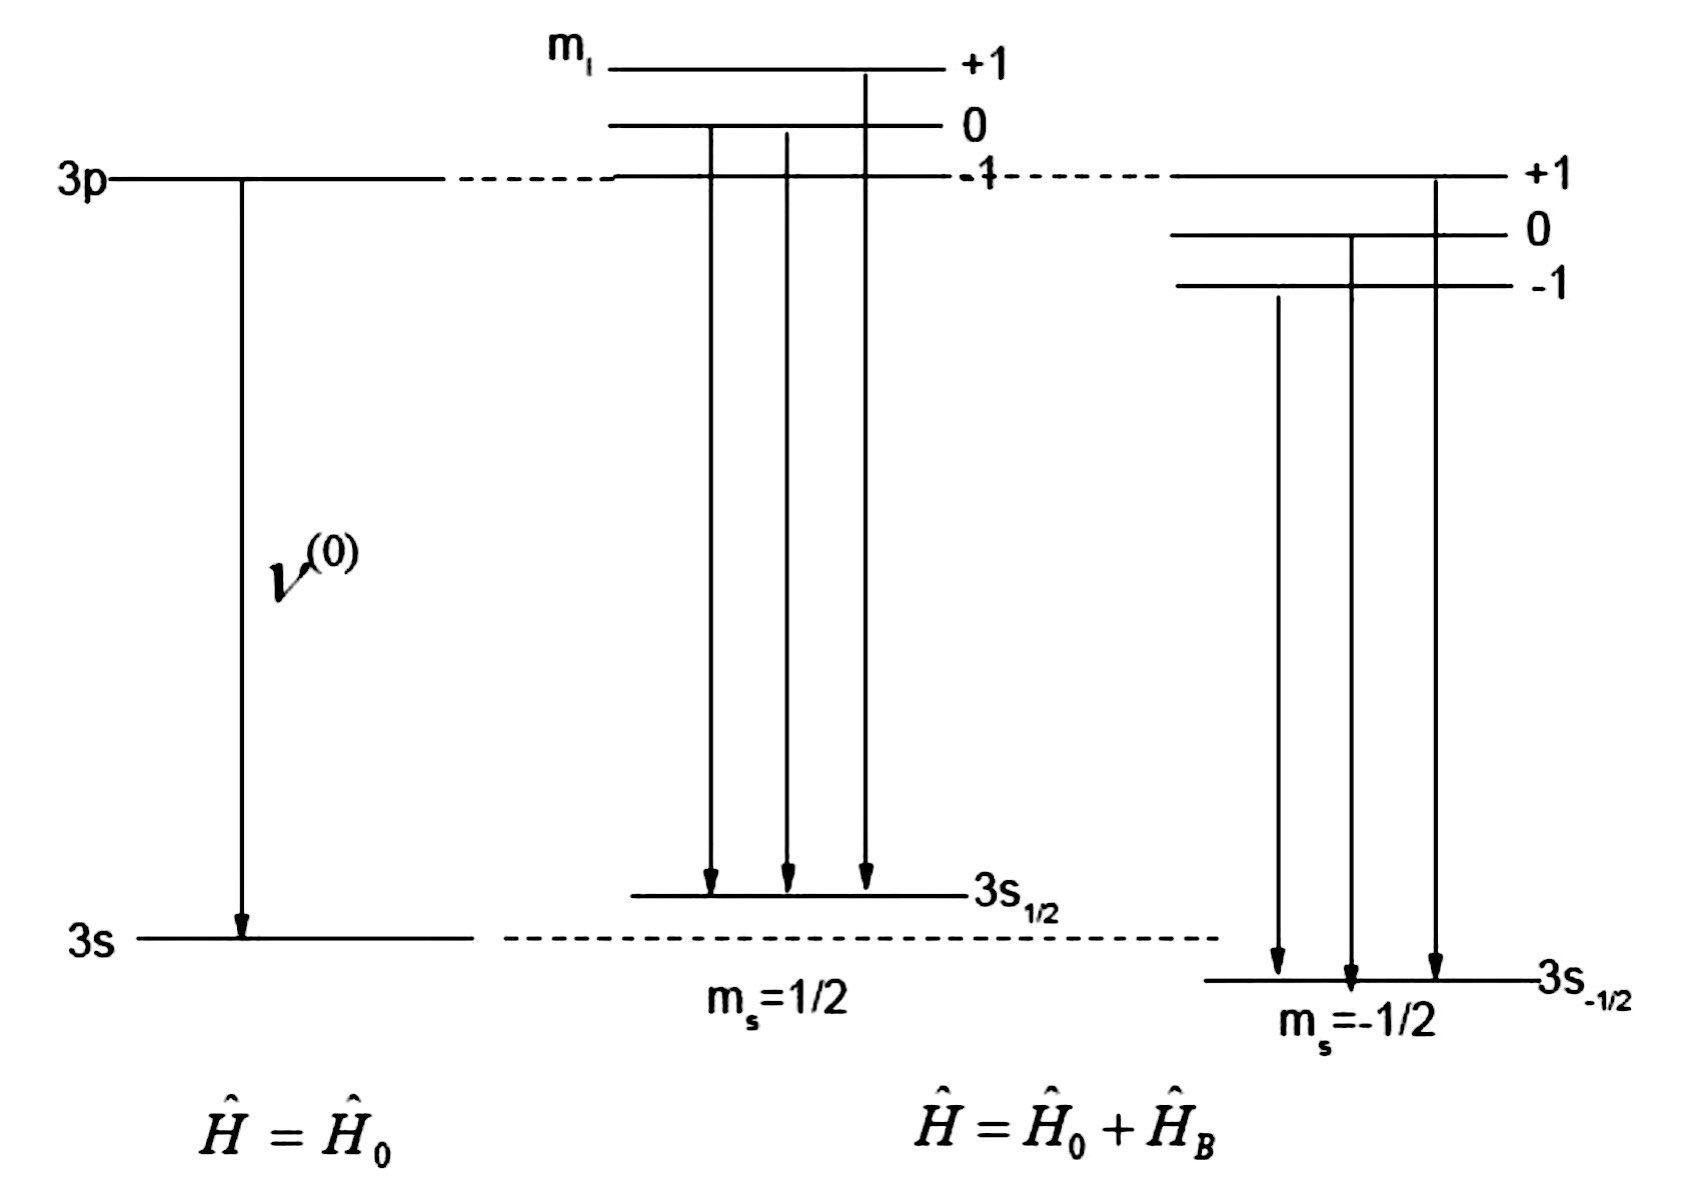
\includegraphics[width=3.5in]{image/Na_jump}
          \caption{钠黄线能谱在强磁场下的劈裂}
        \end{figure}

        其对应的能量本征值为:
        \begin{equation}
          E_{nlml_m} = E_{nl}+(m+2m_s)\hbar\dfrac{eB}{2Mc}
        \end{equation}

        其中, 
        \begin{equation*}
          \begin{aligned}
            n,l&=0,1,2,\ldots\\ 
            m &= -l,-l+1,\ldots,l-1,l\\ 
            m_s &= \pm\dfrac{1}{2}
          \end{aligned}
        \end{equation*}

        根据跃迁选择定则, $\Delta{}m_s=0$. 就可以画出核最外层只有一个电子的元素的跃迁谱线.

        
      \subsection{Landau能级}
        下面, 研究\textbf{二维自由电子}在磁场作用下的特征. 仍然施加沿$z$方向的磁场$B$, 取Landua规范\footnote{对称规范
        情形见 曾谨言 量子力学 卷I , 7.2小节}. 此时$A=(-By,0,0)$. 

        则$xy$方向的二维自由电子的哈密顿量可写为:
        \begin{equation}
          \label{5233:hmdl}
          \hat{H} = \dfrac{1}{2M}\left[\left(\hat{p}_x^2-\dfrac{eB}{c}y\right)^2+\hat{p}_y^2\right]
        \end{equation}

        此哈密顿量下的CSCO可取$\left\{\hat{H}, \hat{p}_x\right\}$. 对应的本征矢为:
        \begin{equation}
          \psi(x,y) = \dfrac{1}{\sqrt{2\pi\hbar}}\mathrm{e}^{i\frac{p_xx}{\hbar}}\varphi(y)
        \end{equation}

        上式中的$p_x$是$\hat{p}_x$的本征值, 其取值范围为整个实数域.

        将上述方程带入\eqref{5233:hmdl}中, 可得:
        \begin{equation}
          \dfrac{1}{2M}\left[\left(p_x-\dfrac{eB}{c}y\right)^2-\hbar^2\dfrac{\mathrm{d}^2}{\mathrm{d}y^2}\right]
          \varphi(y) = E\varphi(y)
        \end{equation}
       
        注意到, 方程中的$p_x$是去掉帽子了的, 是一个具体的数值.

        稍微化简一步得:
        \begin{equation}
          -\dfrac{\hbar^2}{2M}\varphi''(y)+\dfrac{1}{2}M\omega_c^2\left(y-\dfrac{cp_x}{eB}\right)^2\varphi(y) = E\varphi(y)
        \end{equation}

        其中, $\omega_c=\frac{eB}{Mc}$称为回旋频率.

        上式正是平衡位置在$\frac{cp_x}{eB}$的一维谐振子本征方程, 其本征波函数中的$\varphi(y)$对应着一维谐振子的本征波函数.
        其能量本征值为:
        \begin{equation}
          E_n = \left(n+\dfrac{1}{2}\right)\hbar\omega_c\qquad{}n=0,1,2,\ldots 
        \end{equation}

        这个分立的能级被称为Landau能级. 原来自由电子的能级是连续的, 但现加入磁场后在变成了分立的形式.
        在经典图像上

        一定要注意的是, 这里的$E_n$就是系统的总能量. 而不是什么所谓$y$方向分量的能量. 本体系中根本无法将$xy$分量的能量单独分开.

        \textbf{下面讨论该Landau能级的简并度}

        对于有限面积$S$的二维体系. 假设其在$(0,0)$到$(L_x,L_y)$之间的矩形区域. 此时由周期性边界条件\footnote{之所以采用周期性边界条件,
        是考虑到材料边界处仍是材料, 也就是认为材料可以是无限大的.}, 
        $x$方向动量$p_x$取值不再是连续的.
        \begin{equation}
          p_x = \dfrac{2\pi{}n}{L_x}\hbar
        \end{equation}

        从而, 一维谐振子中心坐标可以写作: 
        \begin{equation}
          y_0 = \dfrac{cp_x}{eB} = \dfrac{2\pi{}cn}{eBL_x}\hbar
        \end{equation}

        进而:
        \begin{equation}
          n = \dfrac{L_xy_0eB}{2\pi{}c\hbar}
        \end{equation}

        又由$0\leq{}y_0\leq{}L_y$

        因此,
        \begin{equation}
          f = n_{max}-n_{min} = \dfrac{L_xL_yeB}{2\pi{}c\hbar} = \dfrac{eB}{ch}S
        \end{equation}

        对于无限大平面, 其简并度显然为无穷.

        \textbf{总结磁场下自由电子磁场的特点:}

        \textbf{1.能量色散为平坦的Landau能级}

        \textbf{2. 每个能级高度简并:对于无限的二维体系简并度为无穷;对于有限面积S的二维体系,能级简并度为$f=\dfrac{eB}{ch}S$}

        \textbf{3. 波函数在x方向为扩展态,在y方向为束缚态, 束缚中心为$\dfrac{cp_x}{eB}$, 束缚态波包的宽带与磁场有关.}
        \ \\

        \textbf{再探讨一些其他相关问题.}

        \textbf{1.关于回旋频率的理解}
        
        在经典力学中, 电子在均匀外磁场$B$的作用下, 在平面上做圆周运动. 满足$\vec{F} =\frac{-e}{c}\vec{v}\times \vec{B}$.
        这显然是一个维持电子做圆周运动的向心力形式. 在此力的作用下, 电子做圆周运动的角频率为:
        \begin{equation}
          \omega_c = \dfrac{eB}{Mc}
        \end{equation}

        这正是我们之前所假设的回旋频率$\omega_c$的数值.
        
        \textbf{2.关于Landau能级特征(无色散,高简并度)的理解}

        在经典力学中, 电子在均匀外磁场$B$中运动, 其机械动量为
        \begin{equation}
          \vec{\pi} = M\vec{v} = \vec{P}+\dfrac{e}{c}\vec{A}
        \end{equation}

        根据牛顿第二定律:
        \begin{equation}
          \dfrac{\partial}{\partial{}t}\vec{\pi} + \dfrac{e}{c}\vec{v}\times\vec{B} = 0
        \end{equation}

        于是, $\vec{\pi}+\frac{e}{c}\vec{r}\times\vec{B}$是一个守恒量. 如果磁场沿$z$方向, 则上述守恒量可以化为
        以下两个守恒量:
        \begin{subequations}
          \begin{align}
            \pi_x+\dfrac{eB}{c}y &= \dfrac{eB}{c}\left(y+\dfrac{c}{eB}\pi_x\right)\\
            \pi_y-\dfrac{eB}{c}x &= -\dfrac{eB}{c}\left(x-\dfrac{c}{eB}\pi_y\right)
          \end{align}
        \end{subequations}

        等价地:
        \begin{subequations}
          \begin{align}
            R_y &= y+\dfrac{c}{eB}\pi_x\\
            R_x &= x-\dfrac{c}{eB}\pi_y
          \end{align}
        \end{subequations}

        明显的:
        \begin{equation}
          (x-R_x)^2+(y-R_y)^2 = \dfrac{c^2}{e^2B^2}\left(\pi_x^2+\pi_y^2\right) = \dfrac{2Mc^2}{e^2B^2}H
        \end{equation}

        可见, 电子是以$(R_x,R_y)$为圆心在做圆周运动, 周周运动半径和粒子能量以及磁场强度有关. 除了守恒量$\vec{R} = (R_x,R_y)$之外, 
        还有守恒量:
        \begin{equation}
          \Lambda_z = (x-R_x)\pi_y-(y-R_y)\pi_x = \dfrac{2Mc}{eB}H
        \end{equation}
        
        这正是电子相对于$\vec{R}$的轨道角动量!

        将上述经典图像过度到量子力学, 使用算符代替相应的力学量. 
        \begin{equation}
          \begin{aligned}
            \hat{\pi}_x &= \hat{p}_x + \dfrac{e}{c}A_x\\
            \hat{\pi}_y &= \hat{p}_y + \dfrac{e}{c}A_y\\
            \hat{R}_y  &= \hat{y}+\dfrac{c}{eB}\hat{\pi}_x\\
            \hat{R}_x &= \hat{x}-\dfrac{c}{eB}\hat{\pi}_y\\
            \hat{\Lambda} &= \left(\hat{x}-\hat{R}_x\right)\hat{\pi}_y-\left(\hat{y}-\hat{R}_y\right)\hat{\pi}_x \\
            &= \dfrac{2Mc}{eB}\hat{H}
          \end{aligned}
        \end{equation}

        不难看出:
        \begin{equation}
          \begin{aligned}
            &\left[\hat{H},\hat{\pi}_x\right] \ne 0\\
            &\left[\hat{H},\hat{\pi}_y\right] \ne 0\\
            &\left[\hat{\pi}_x,\hat{\pi}_y\right] = -\dfrac{i\hbar{}e}{c}B
          \end{aligned}
        \end{equation}

        可见, 机械动量$\left(\hat{\pi}_x,\hat{\pi}_y\right)$并非守恒量. 在本征态上他们的取值是不确定的. 但可以计算出, 他们的平均值
        在本征态上是零\footnote{束缚态动量平均值为0}.

        再来研究$\hat{R}_x$和$\hat{R}_y$. 对这两个算符, 有:
        \begin{equation}
          \begin{aligned}
          \left[\hat{H}, \hat{R}_x\right] &= 0\\
          \left[\hat{H}, \hat{R}_y\right] &= 0\\
          \left[\hat{R}_x,\hat{R}_y\right] &= \dfrac{i\hbar{}c}{eB}
          \end{aligned}
        \end{equation}

        $\hat{H}$分别与$\hat{R}_x$, $\hat{R}_y$有共本态系, 但$\hat{R}_x$, $\hat{R}_y$互相不对易, 说明他们没有共本态系.
        只用$x$或$y$一个参量就可以确定能量, 那么此体系的能级必然是简并的. 我们之前求出的态正是$\left\{\hat{H},\hat{y}\right\}$
        对应的本征态, 本征值为$E_n$和$y_0$. 并且在该本征态上, $\hat{R}_x$的期望为0. 这说明, 该本征态电子圆周运动的圆心在
        $(0,y_0)$处.

        \textbf{最后总结和对比二维自由电子在磁场下的特征.}

        \begin{table}[H]
          \centering
          \begin{spacing}{2.5}
          \caption{二维自由电子在磁场下的特征}
          \begin{tabular}{c|c|c}
            \toprule
                       & 二维薛定谔电子 & 二维Dirac电子\\ 
            \hline
            无磁场时色散 &$E=\dfrac{\hbar^2}{2m}k^2$ & 线性\\
            \hline
            磁场下平坦的Landau能级 & $E_n = \left(n+\dfrac{1}{2}\right)\hbar\omega_c$ & %
            $E_{\pm}=\pm\dfrac{\sqrt{2}\hbar\gamma}{l_B}\sqrt{n}$\\ 
            \bottomrule 
          \end{tabular} 
          \end{spacing}
        \end{table}

        上表中磁场下的Dirac电子正是我们在式\eqref{Dirac:ele}中讨论的磁场中的石墨烯材料.
        
      \subsection{量子Hall效应}
        量子Hall效应是指在低温下, 二维自由电子气在强磁场中出现的Hall电阻(电导)率的量子化现象. 
        其主要原因是:
        \begin{enumerate}[1.]
          \item 实验材料在某个方向上受限制使边态出现, 并产生色散;
          \item 工作电子态处于两个Landau能级之间, 体态不参与工作, 靠边态传播, 不受体内杂质影响.
          \item 轨道角动量守恒, 不受一般杂质(不破坏角动量守恒的)散射.
        \end{enumerate}

      \subsection{三维自由电子在磁场下的Landau带}

       对于三维自由电子, 其哈密顿量为:
       \begin{equation}
        \hat{H} = \dfrac{1}{2M}\left[\left(\hat{p}_x^2-\dfrac{eB}{c}y\right)^2+\hat{p}_y^2\hat{p}_z^2\right]
       \end{equation}
        
       取CSCO为$\left\{\hat{H}, \hat{p}_x. \hat{p}_z\right\}$, 那么其共本态为:
       \begin{equation}
         \Psi(x,y,z) = \dfrac{1}{2\pi\hbar}\mathrm{e}^{i\frac{p_xx+p_zz}{\hbar}}\varphi(y)
       \end{equation}

       本征方程为:
       \begin{equation}
         \dfrac{1}{2M}\left[\left(p_x-\dfrac{eB}{c}y\right)^2-\hbar^2%
         \dfrac{\mathrm{d}^2}{\mathrm{d}t^2}+p_z^2\right]\varphi(y)=E\varphi(y)
       \end{equation}

       能量本征值为:
       \begin{equation}
         E_n = \left(n+\dfrac{1}{2}\right)\hbar\omega_c+\dfrac{p_z^2}{2M}\qquad{}n=0,1,2,\ldots
       \end{equation}

       可见, 这是一个螺旋线模型.
  \part{课外拓展}
    \section{多粒子体系}
      \subsection{双粒子体系}

      \subsection{原子}

      \subsection{固体}


    \section{量子纠缠和量子隐形远程传态} 
      
\end{spacing}
\end{document}